\documentclass{fheadnote}

\usepackage{amsmath}
\usepackage{amsfonts}
\usepackage{amssymb}
\usepackage{makeidx}
\usepackage{graphicx}
\usepackage{url}
\usepackage{verbatim}
\usepackage{textcomp}
\usepackage{footnote}
\usepackage{hyperref}
\usepackage{lscape}

\begin{document}

\begin{titlepage}

   \fheadnote{2011/001}
   \date{\today}

   \title{Toy study on MR/R behavior}

   \begin{Authlist}
      Yi Chen
      \Instfoot{Institute}{California Institute of Technology}
   \end{Authlist}

   % \collaboration{FHead}

  \begin{abstract}
     A series of toy studies has been carried out to gain intuition of the kinematic magic bullet
     variables from Chris.  This document is an attempt to summarize the main points coming out from the toys.
  \end{abstract}

\end{titlepage}

\setcounter{page}{2}

\tableofcontents
\clearpage

\section{Overview}

\subsection{Background story}

Since this is personal note, I won't bother with doing research on background knowledge etc.


\subsection{Definition of $M_R$, $M_R^T$ and $R$ as copied from Chris' paper}

Let $P_1$ and $P_2$ be the four-momenta of the two jets and $\overrightarrow{M}$ be the transverse missing energy in the event, $M_R$ is defined as

\begin{equation}
M_R = 2 \sqrt{\dfrac{(P_1^0 P_2^3 - P_1^3 P_2^0)^2}{(P_1^3 - P_2^3)^2 - (P_1^0 - P_2^0)^2}},
\end{equation}

while the ``transverse version'' is defined as

\begin{equation}
M_R^T = \sqrt{\dfrac{1}{2} |\overrightarrow{M}| (P_{1T} + P_{2T}) - \dfrac{1}{2} \overrightarrow{M} \cdot (\overrightarrow{P_{1T}} + \overrightarrow{P_{2T}})},
\end{equation} 

and a massless ratio $R$ is formed by taking the ratio of these.


\subsection{Reasoning behind $M_R$ as I see it}

The first step in understanding it is to think through why this variable is as it is, so let me try to restate the reasoning behind $M_R$.

\begin{enumerate}
\item During collision it is usual for the hard process system to be boosted in the z direction, while in the transverse direction the boost goes roughly as $q^2$ and is small in general,
so for any variable we want to use it better be z-boost invariant.  Let's work in a frame where the hard process does not have a total z direction boost.
\item We focus on the case that two heavy objects are pair-produced, and each decays into a heavy invisible particle and some visible ones.
\item Since the two heavy object is not created by an on-shell resonance particle, the boost of heavy object in the hard-process-CM frame is preferrably small.
The chance of high boost is highly suppressed since the spectrum is fast falling.  Let's assume now that it is not boosted.
\item Now, all we see is two heavy objects of same size.  Since we do not know anything about the invisible objects (in $M_R$ at least), let's assume they are exactly the same as the visible partner but
in opposite direction.  In this case if we form the invariant mass of the heavy object, the central value of $M_R$ can be predicted.
\item Experimentally, what we can do to find this frame is to solve algebraic equation and find a frame where the two heavy object has the same magnitude of momentum.
\end{enumerate}


\subsection{List of toys performed so far}

There are two scenarios being considered.  One is leptoquark-like, heavy objects are pair-produced, which then decays into a visible object (b-meson) and an invisible object (neutrino).
Another scenario is ttbar-like, where the W's decay leptonically.

\begin{enumerate}
\item[1] LQ.  Changing boost of heavy object in the hard-process-CM frame.
\item[2] LQ.  Changing mass of various objects.
\item[3] LQ.  Smearing momentum and direction of final particles.
\item[4] LQ.  Check explicitly that the variables are invariant under z-direction boost.
\item[5] LQ.  Investigate how the variables react under transverse boost.
\item[5-2] LQ.  Under transverse boost, there are some strange feature in the $R-M_R$ plane.  This is an attempt at plotting out allowed phase spaces in each region.
\item[6] ttbar.  Changing mass of various objects, assume we know which b and which lepton are together
\item[7] ttbar.  Changing mass of various objects, group things into hemispheres.
\item[8] LQ.  Adding underlying event di-jet.  The dijets can have z-boost.  $M_R$ and $R$ formed from the leading two jets
\item[9] LQ.  Same as previous one, but with hemispheres.
\item[10] LQ.  ISR jet balancing the whole system.
\item[11] LQ.  Hard-process-only generator-level events from PYTHIA8.
\item[12] LQ.  Map out what the allowed phase space are for each R cut - in the hard-process-CM-frame.
\item[13] LQ.  ISR jet balancing the whole system, limiting ISR direction to be transverse.
\item[14] LQ.  Different acceptance cut ($\eta$ range).
\item[15] LQ.  Effect of holes in detector.
\end{enumerate}


\subsection{A couple technical notes on implementation}

All the particles are treated as scalars since I don't have time to figure out how to get the distribution correctly yet.
In ttbar toys there will be spin-correlations in real life, but in leptoquark case we're focusing on scalar leptoquarks for now, so this is okay.
For each decay (W to l nu, t to b W, LQ to b nu, glu to LQ LQ, glu to ttbar), a random angle is drawn in the mother particle rest frame, and then boosted to the next level.


\section{Highlights}

\subsection{MRToy 4, checking z-boost invariance}

As shown in figure \ref{Figure_MRToy4}, there is negligible difference between two cases: one with
large boost in z direction and another one without any boost.  The difference between the two
cases are believed to be merely statistical fluctuations.  In the complete toy study there are a list
of other boost possibilities considered, but the result is exactly the same (ie., fluctuating around
the same value.)  Maybe I should take this out of the highlight section?

\begin{figure}[htbp]
   \centering
   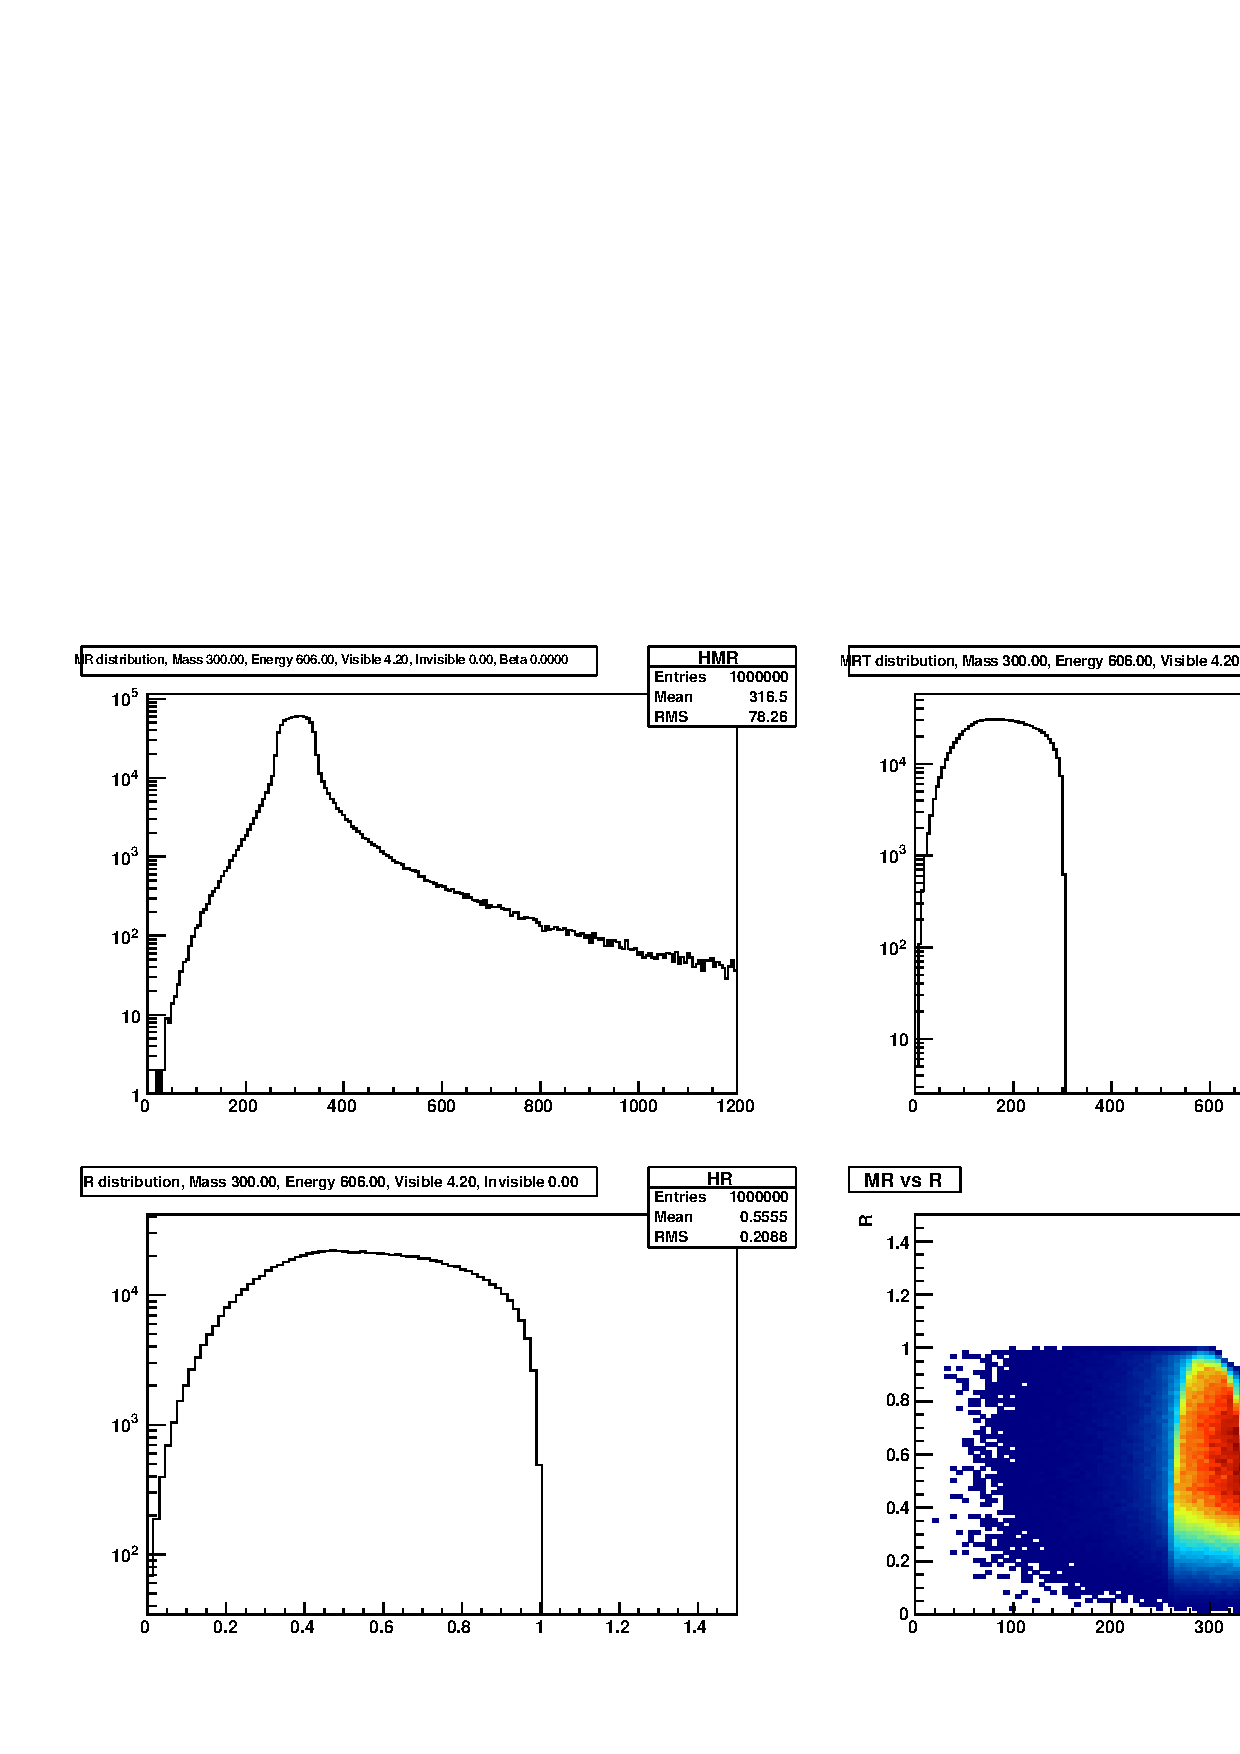
\includegraphics[width=7cm]{Figures/MRToy4_NoBoost}
   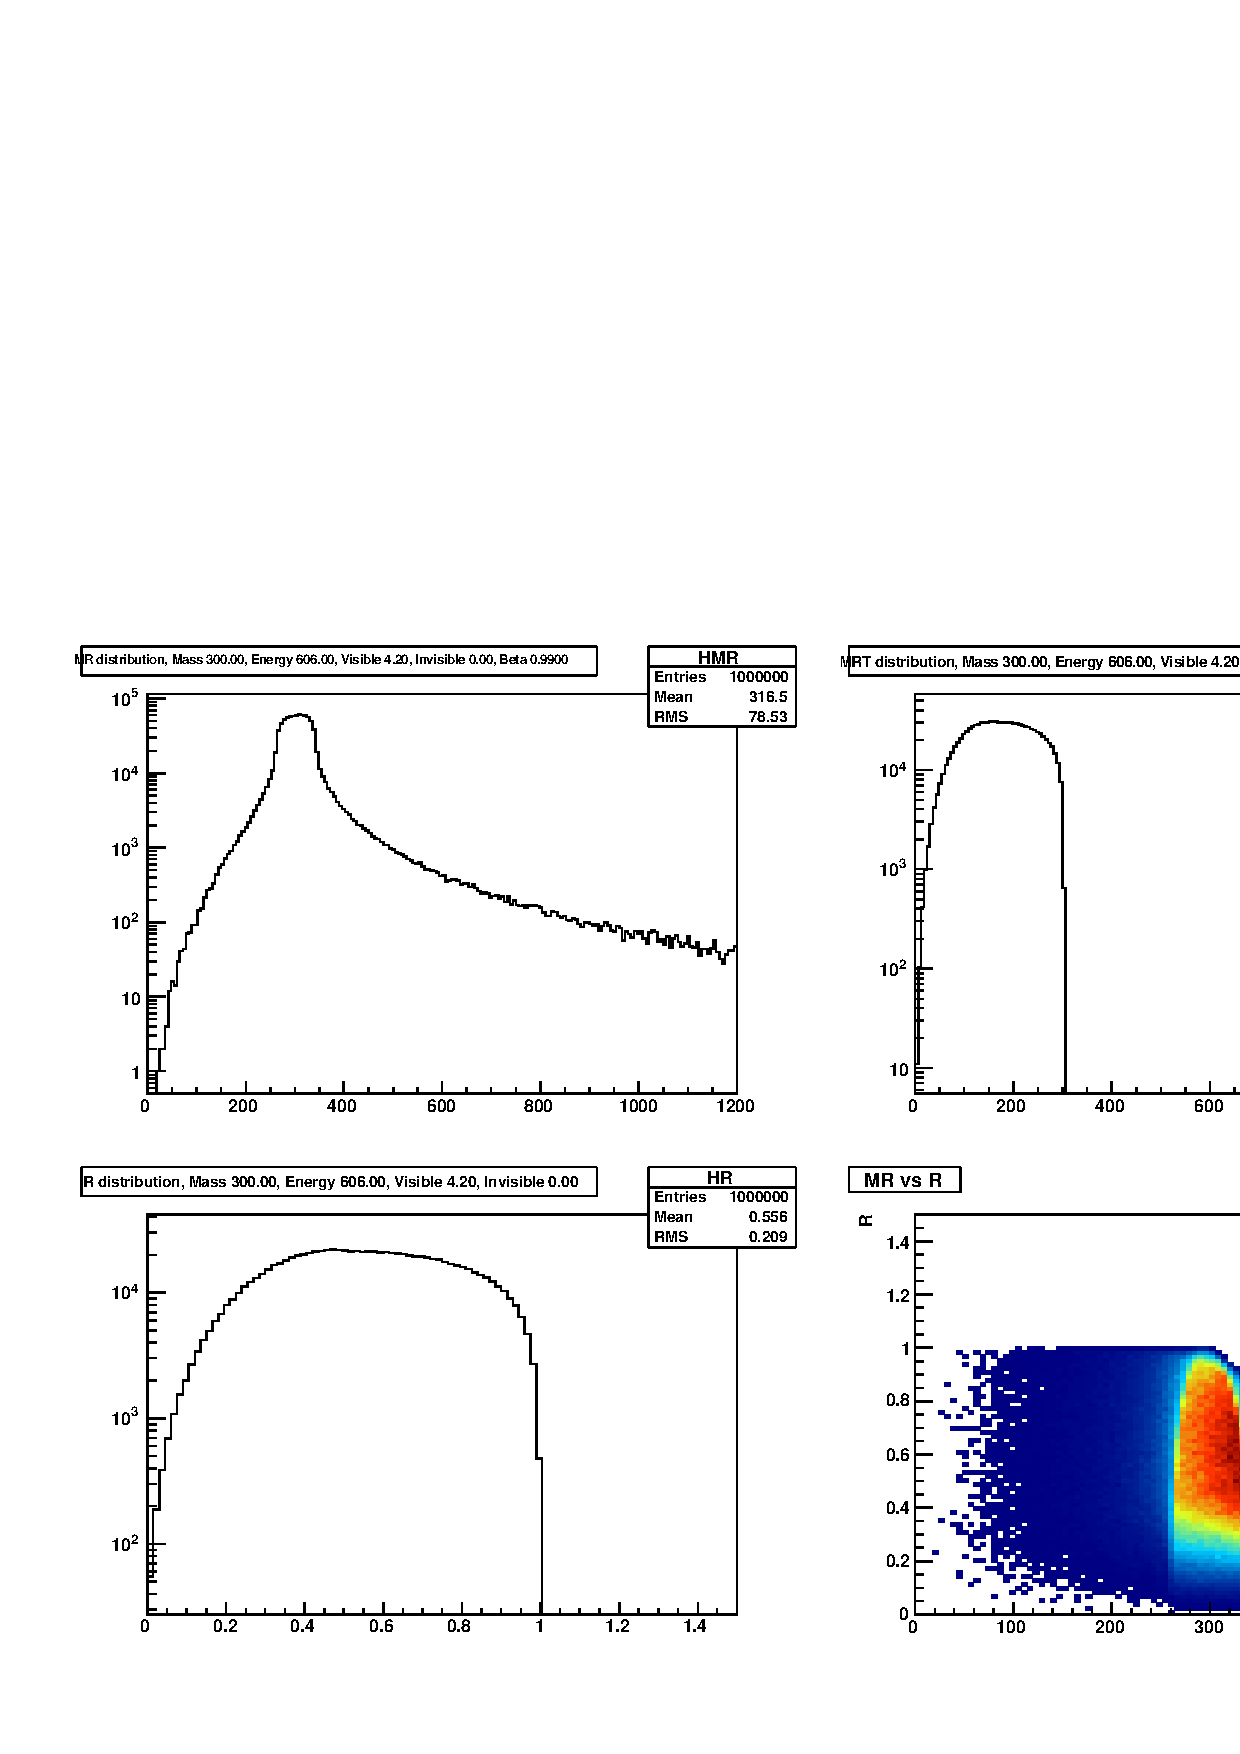
\includegraphics[width=7cm]{Figures/MRToy4_LargeBoost}
   \caption{MRToy 4, verifying explicitly that things are z-direction boost invariant.
   First four plots are with no boost, while the right-hand side four are with large z-drection boost
   (beta = 0.99)}
   \label{Figure_MRToy4}
\end{figure}

\subsection{MRToy 2, varying masses of various objects}

This toy study is interesting in that it confirms my reasoning behind designing for $M_R$ variable.
I wasn't following too closely the text and tried to come up with something that roughly explains the designed variable by Chris.
So as the mass of different objects are varied, central value of $M_R$ will change also.
In figures \ref{Figure_MRToy2}, every bin in the histogram is a toy experiment with 10000 or so tries to get the
central value of $M_R$.
The overlaid line is the value I got from the hypothesis --- assuming the invisible partner is the same and opposite (in direction) of
the visible objects, and calculate the invariant mass of those.
And it is right on spot, which is good.

\begin{figure}[htbp]
   \centering
   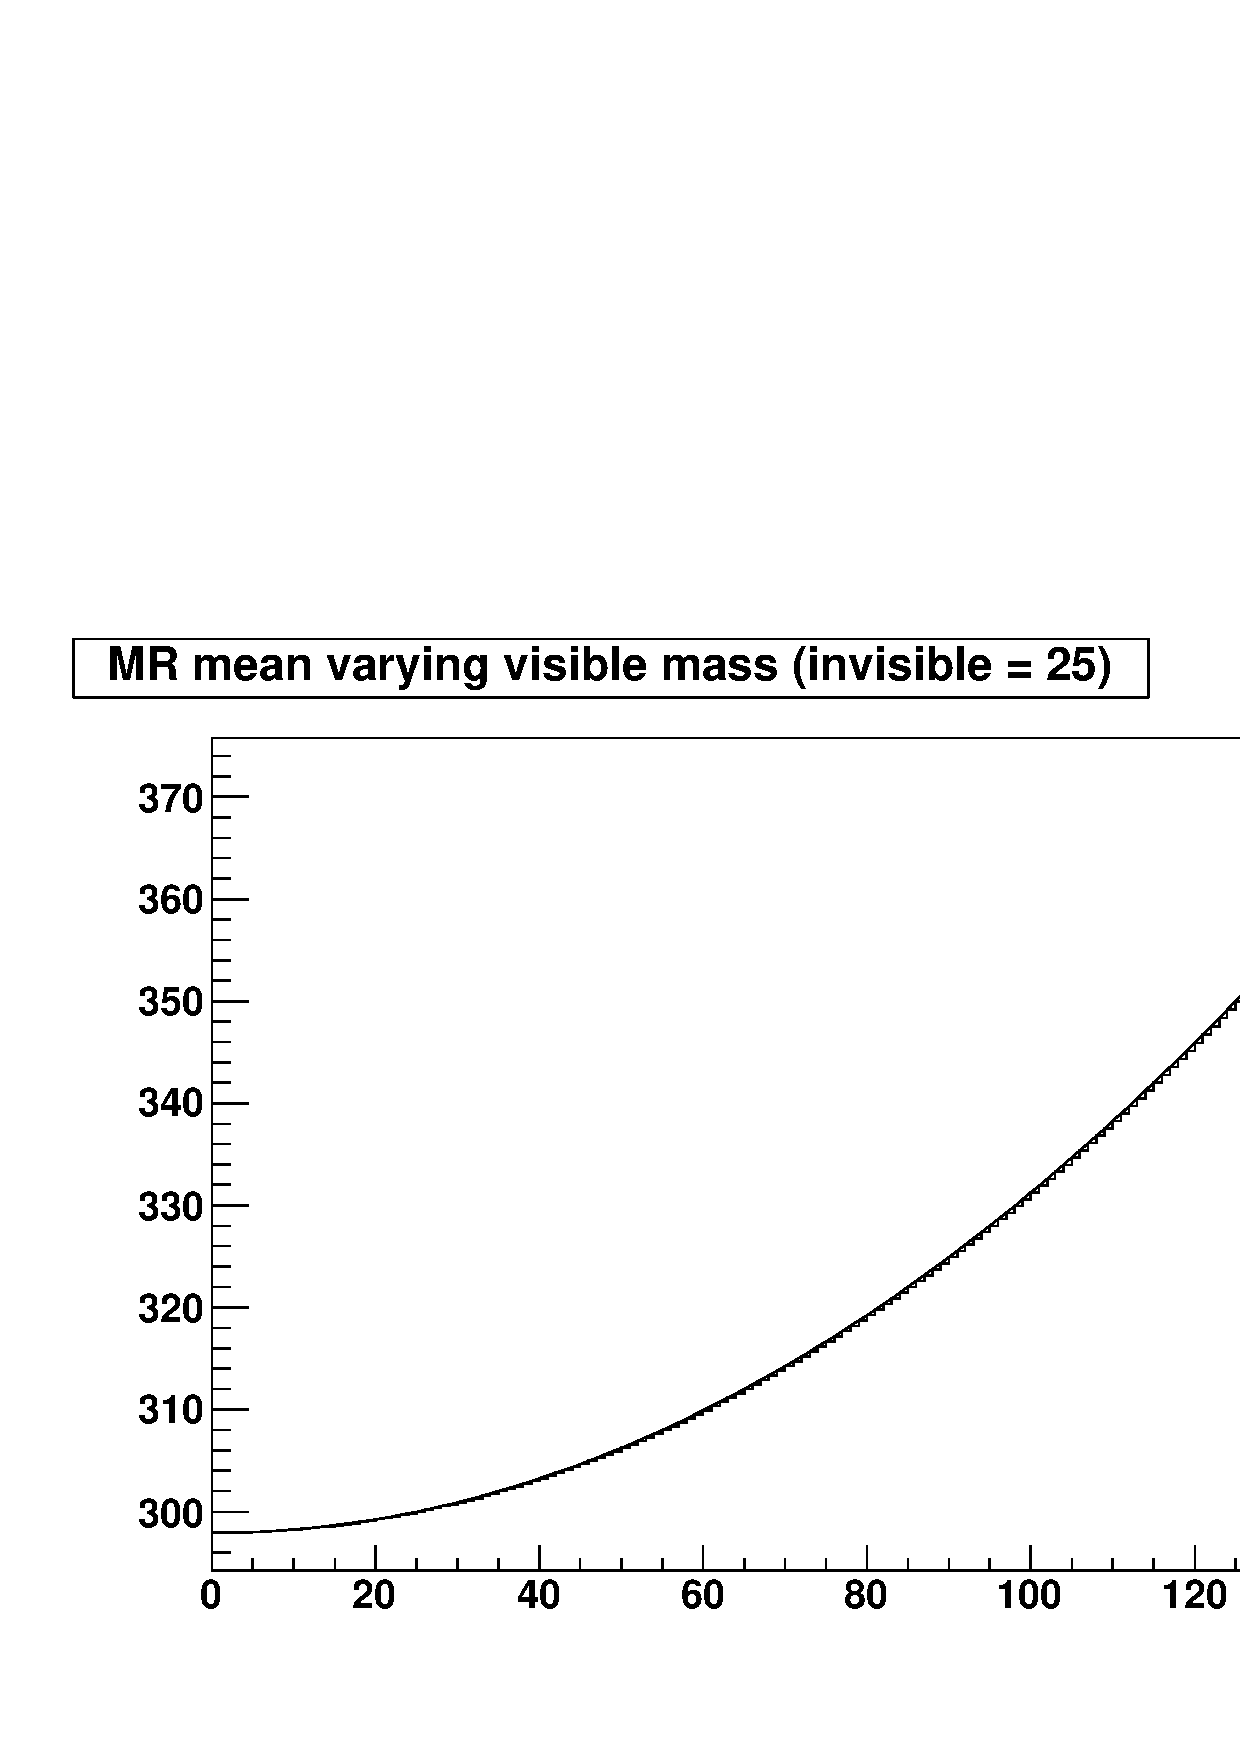
\includegraphics[width=7cm]{Figures/MRToy2_Summary1}
   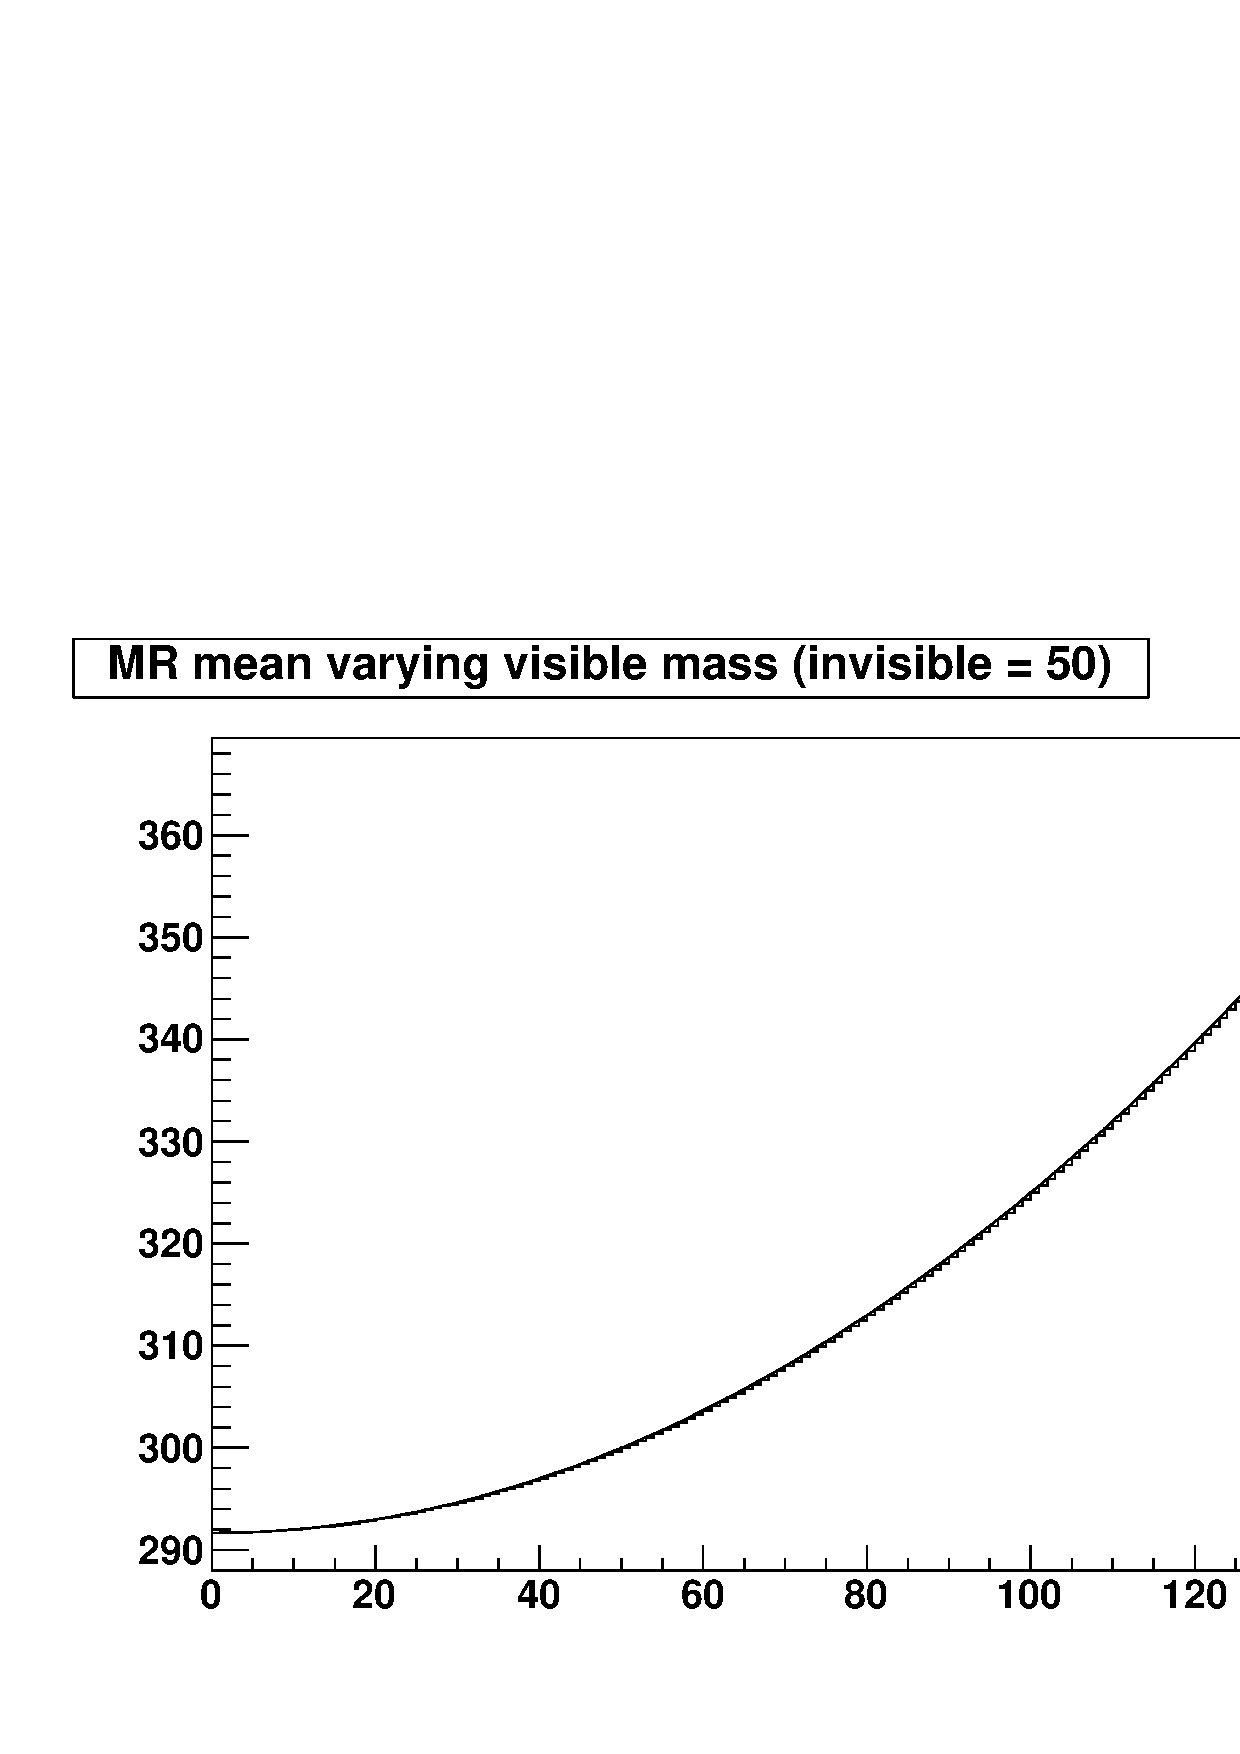
\includegraphics[width=7cm]{Figures/MRToy2_Summary2}\\
   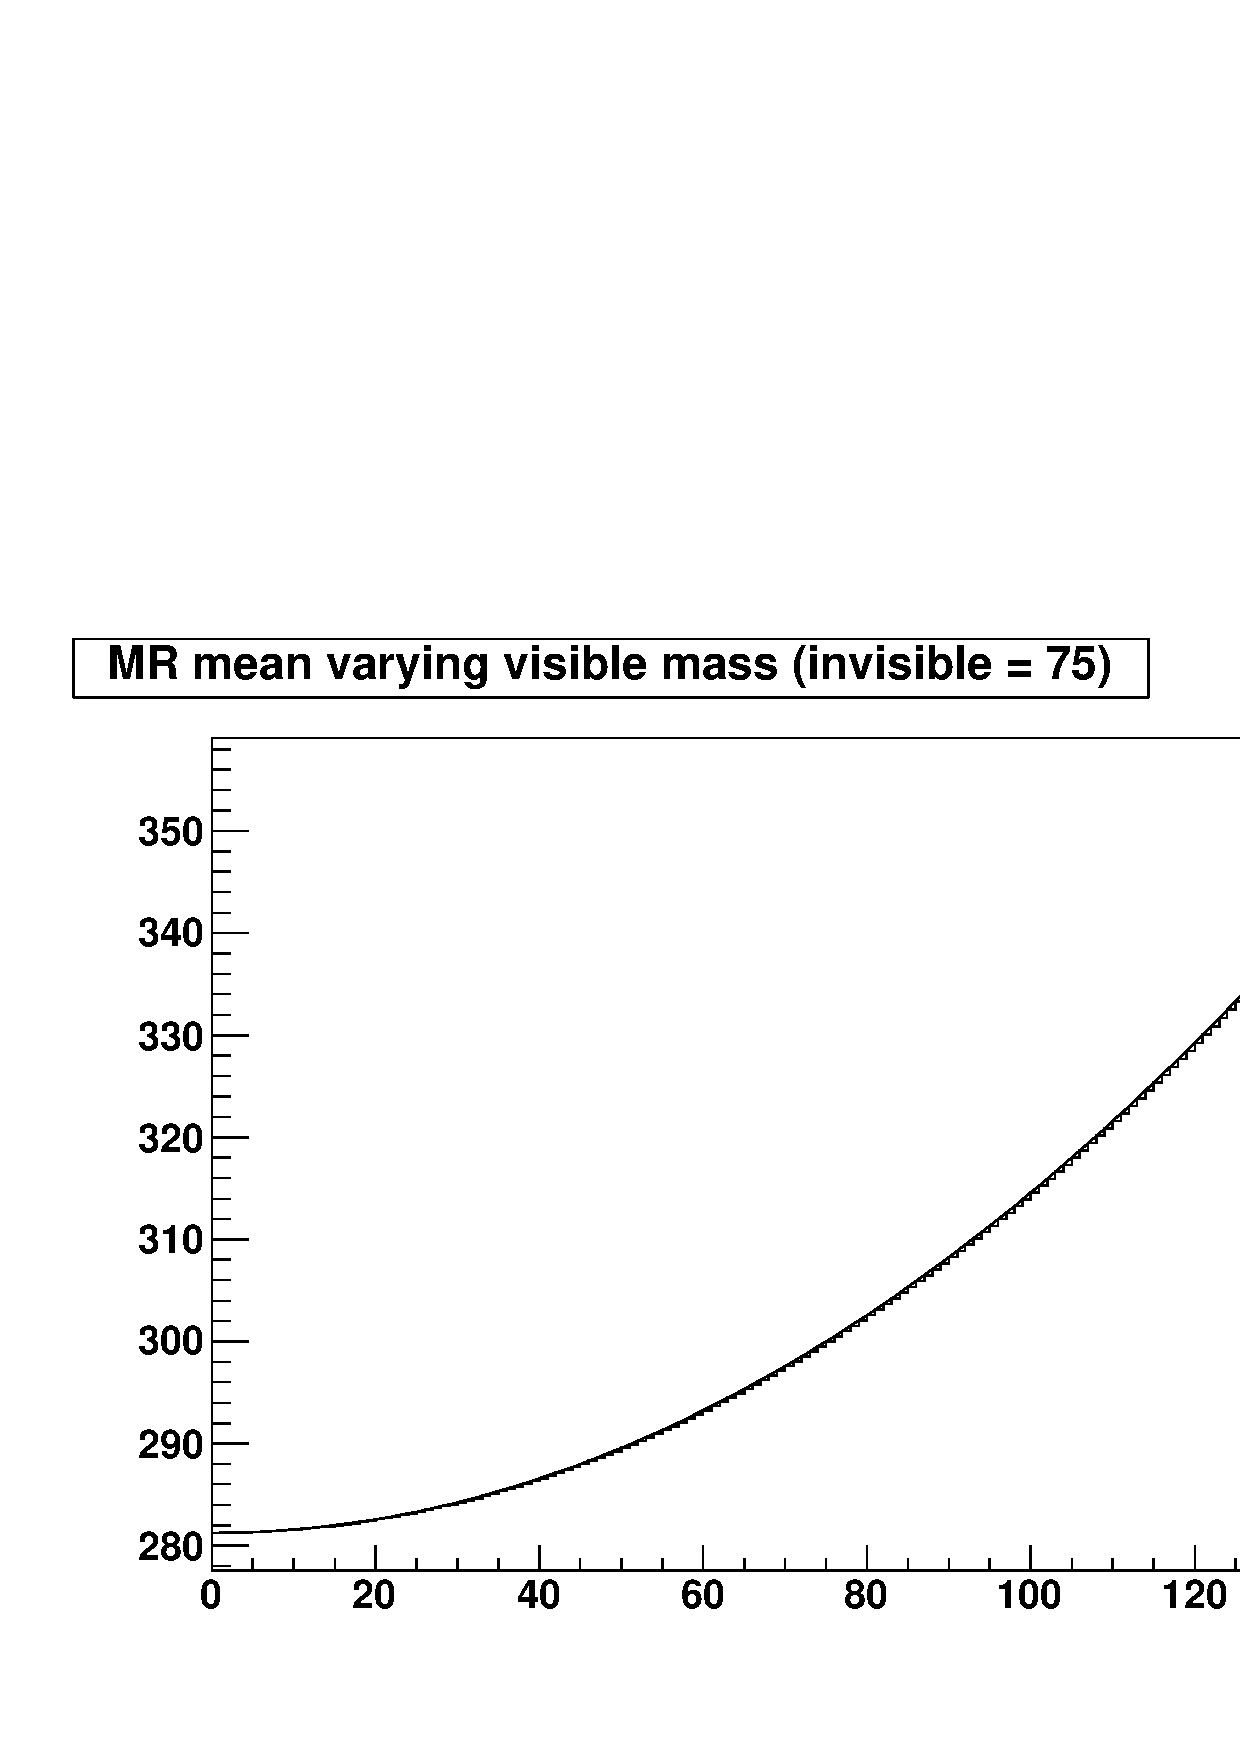
\includegraphics[width=7cm]{Figures/MRToy2_Summary3}
   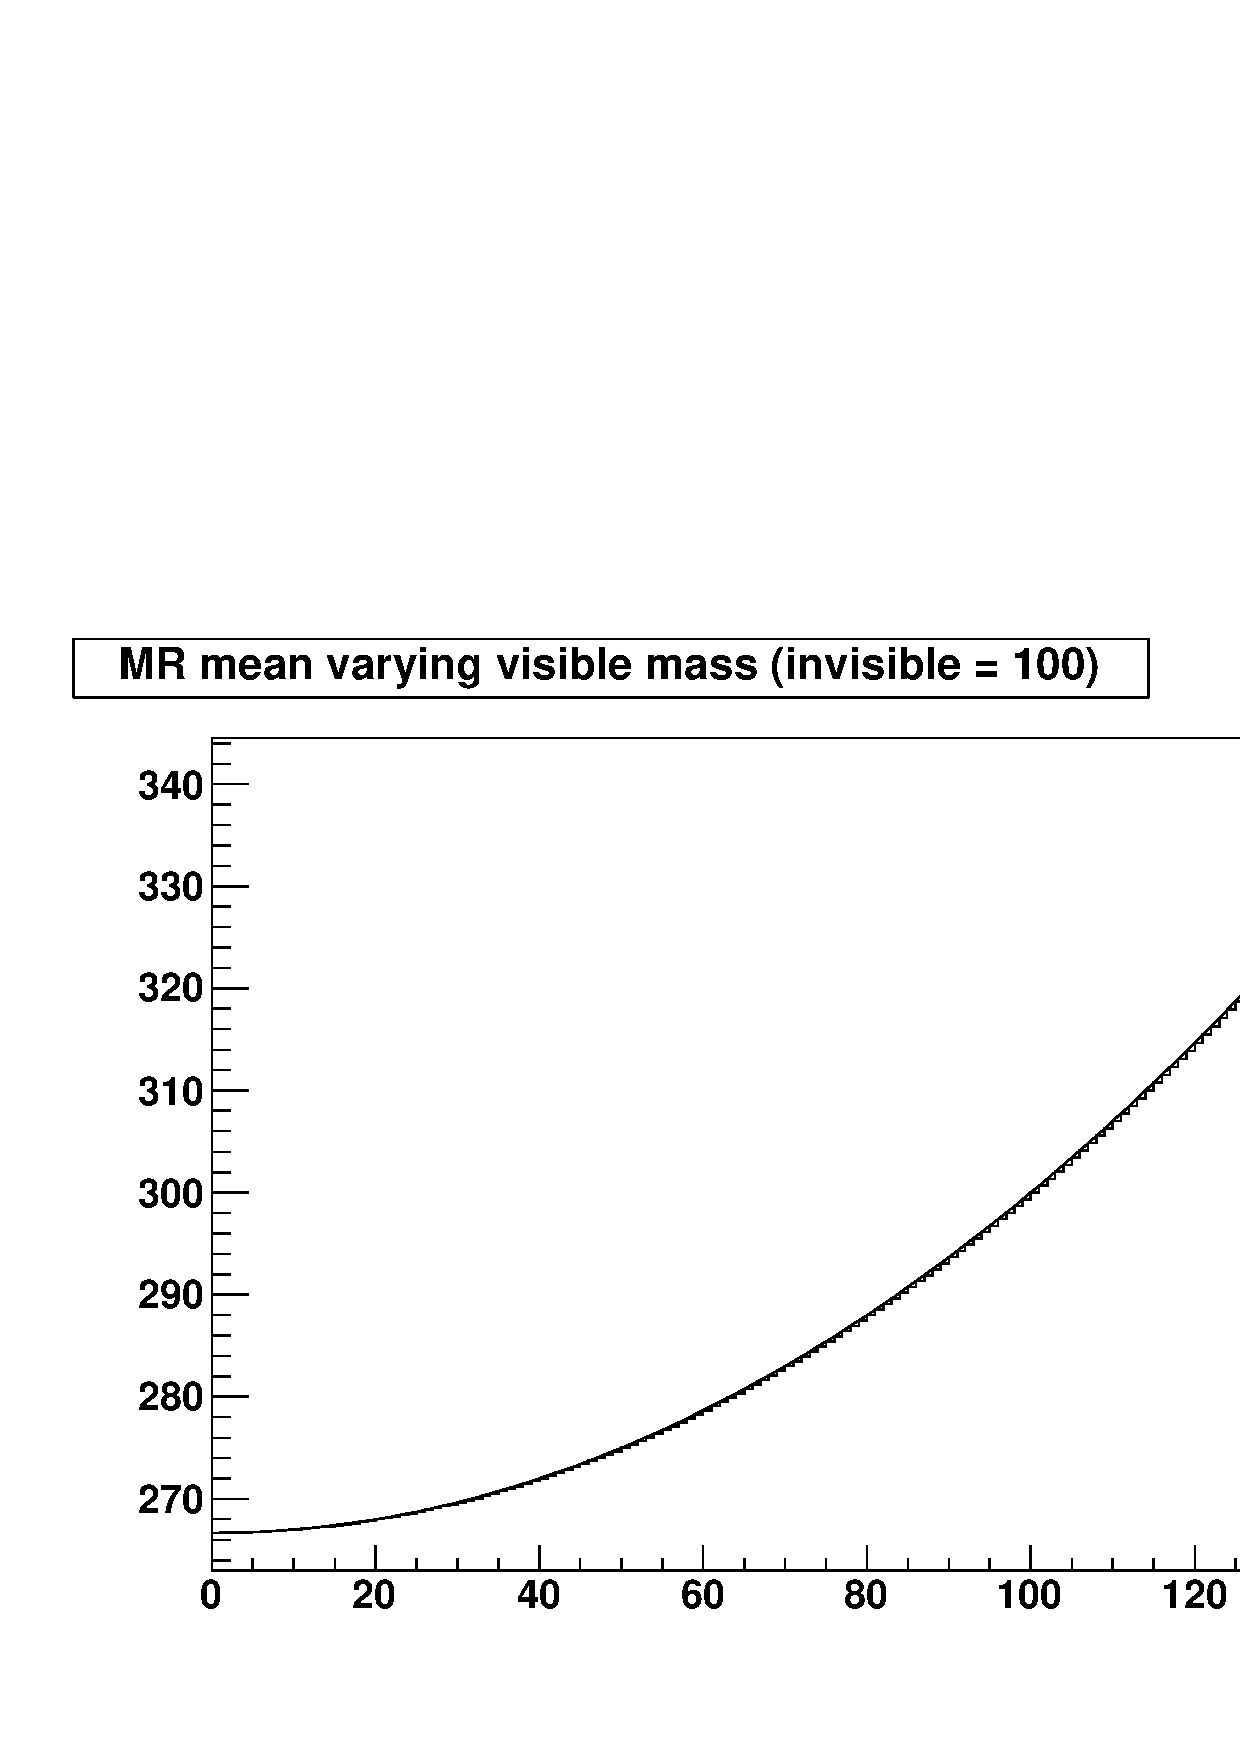
\includegraphics[width=7cm]{Figures/MRToy2_Summary4}
   \caption{MRToy 2, $M_R$ central value vs. predicted value from hypothesis, varying visible and invisible masses.  They show nice agreement.}
   \label{Figure_MRToy2}
\end{figure}

\subsection{MRToy 7, Group things into hemisphere for ttbar scenario}

It further confirms the hypothesis that we made an assumption that the invisible part of the decay chain is exactly the same as the visible part.
In retrospect this is probably the best we can do without going into specifics: there are two objects, and if they each come from a heavy object,
and we know there is an invisible part, an assumption about the invisible particles has to be made, one way or another.
Without making it model-dependent, let's assume that it is the same as the visible ones.



\subsection{MRToy 12, mapping out angular distributions for each $R$ cut}

Variable $R$ is a pure topological cut.  It is therefore instructive to map out what the available phase space is for each $R$ value.
Here the setup is in the heavy-process-CM frame, $\gamma_{CM}$ is 1 for simplicity.  No $\eta$ phase space cut.
The visible particles are parameterized in terms of $\theta$ angle, as well as the $\Delta\phi$ between them, since there is
one redundant degree of freedom in the $\phi$ angles.
The invisible ones are the exact opposite of visible ones, so there is no extra degree of freedom in the direction of those particles.
Figure \ref{Figure_MRToy12_Raw} shows the allowed particle directions in different regions of $R$.
In each block, the upper two panels are the directions of the two particles plotted together,
and the remaining 6 panels show where the visible particle can move if we fix the other one to some $\theta$ range.
It takes some time to decode the figures, but there is a sketch shown in figure \ref{Figure_MRToy12_Summary}
summarizing the findings.

\begin{landscape}
\begin{figure}[htbp]
   \centering
   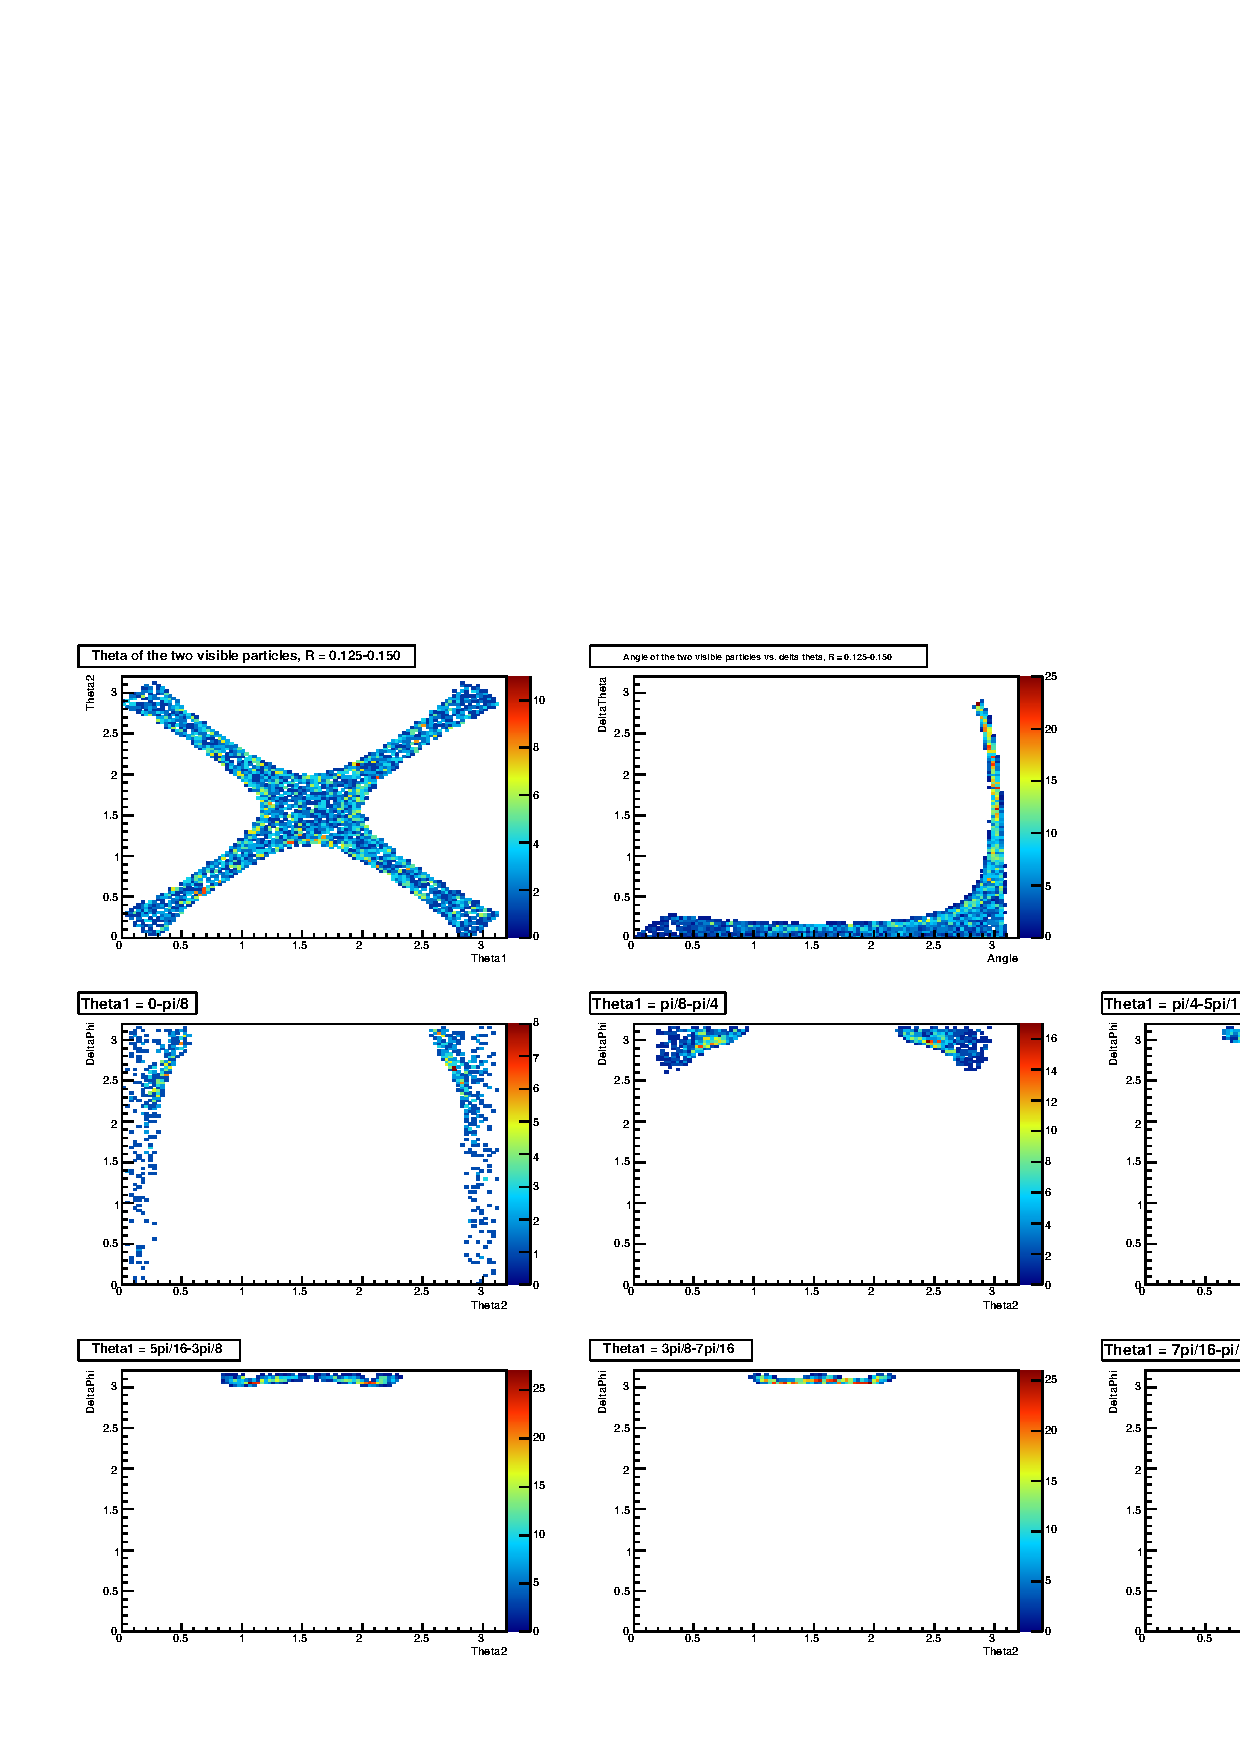
\includegraphics[width=11cm]{Figures/MRToy12_RPhaseSpace_SmallR}
   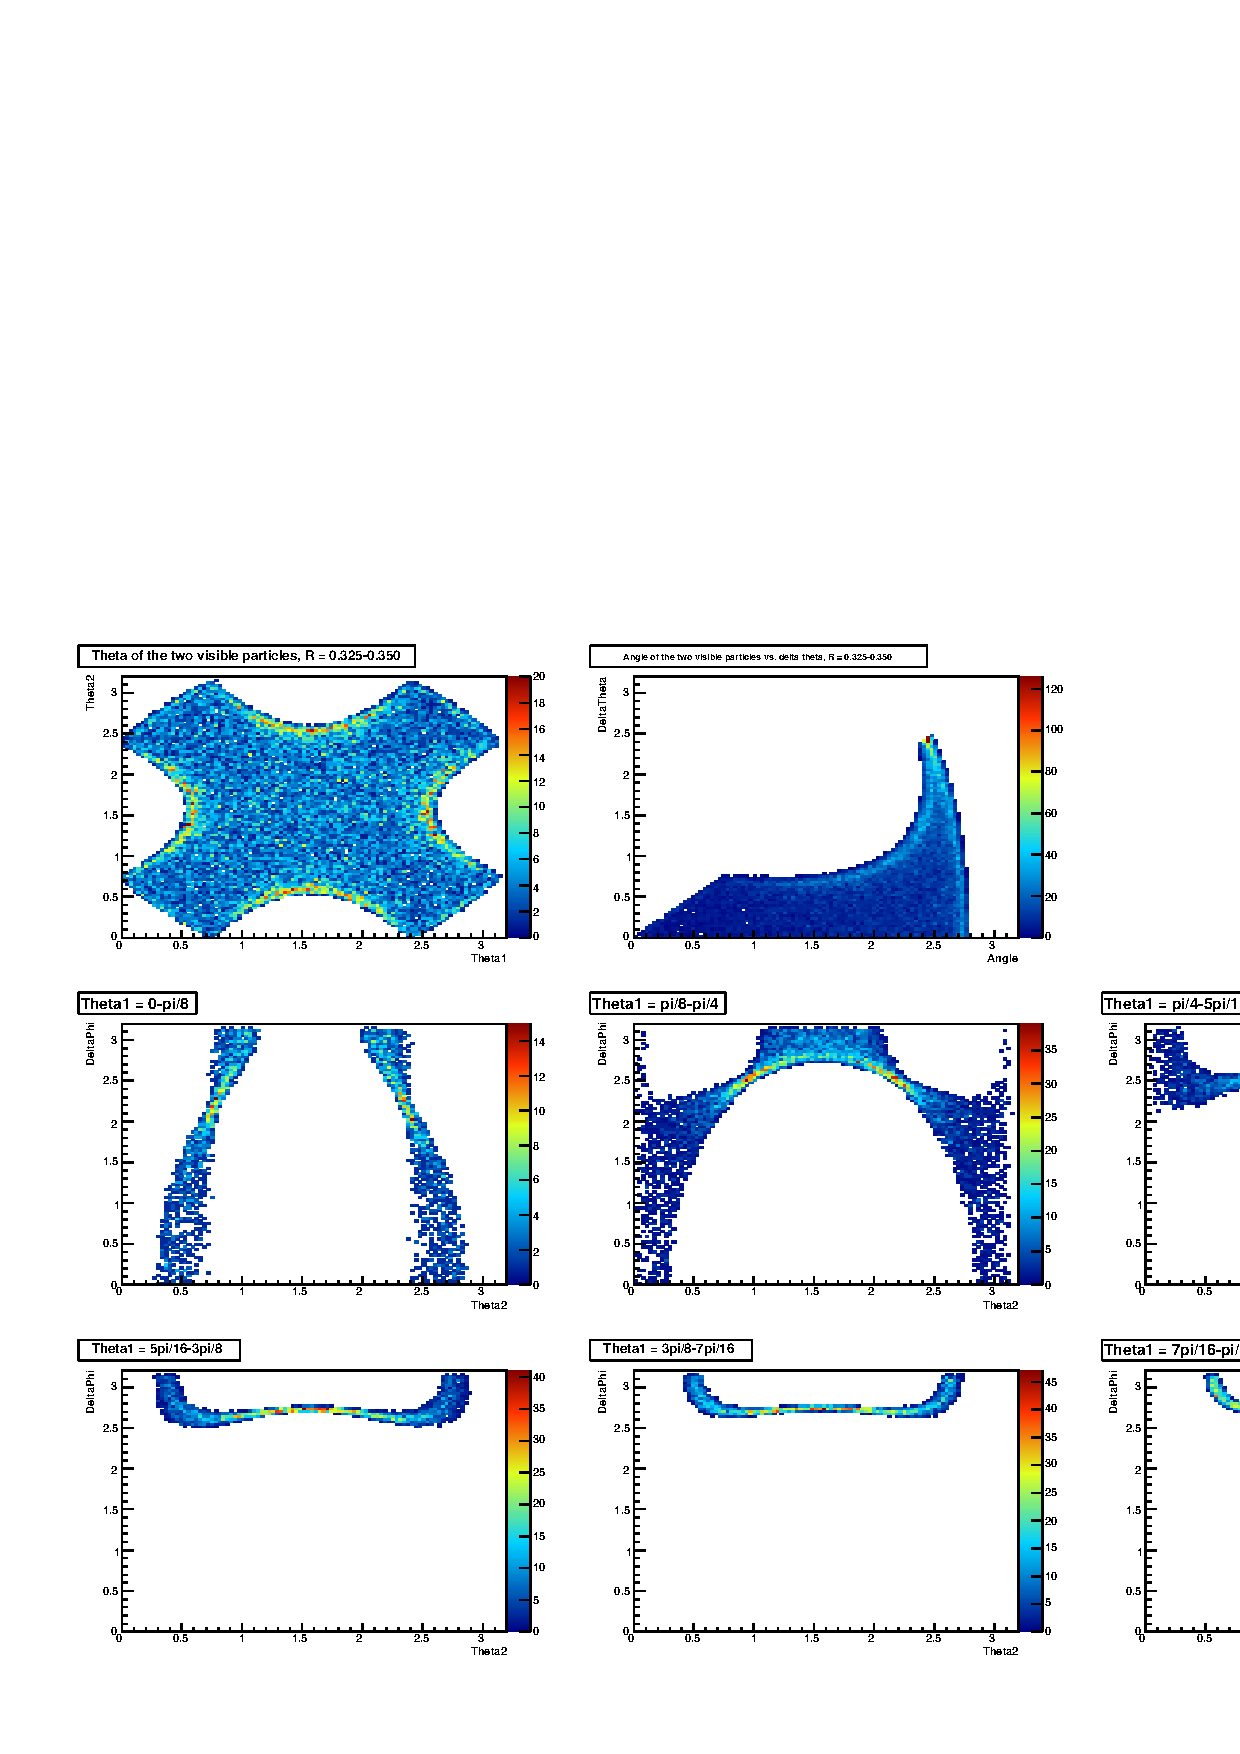
\includegraphics[width=11cm]{Figures/MRToy12_RPhaseSpace_IntermediateR}\\
   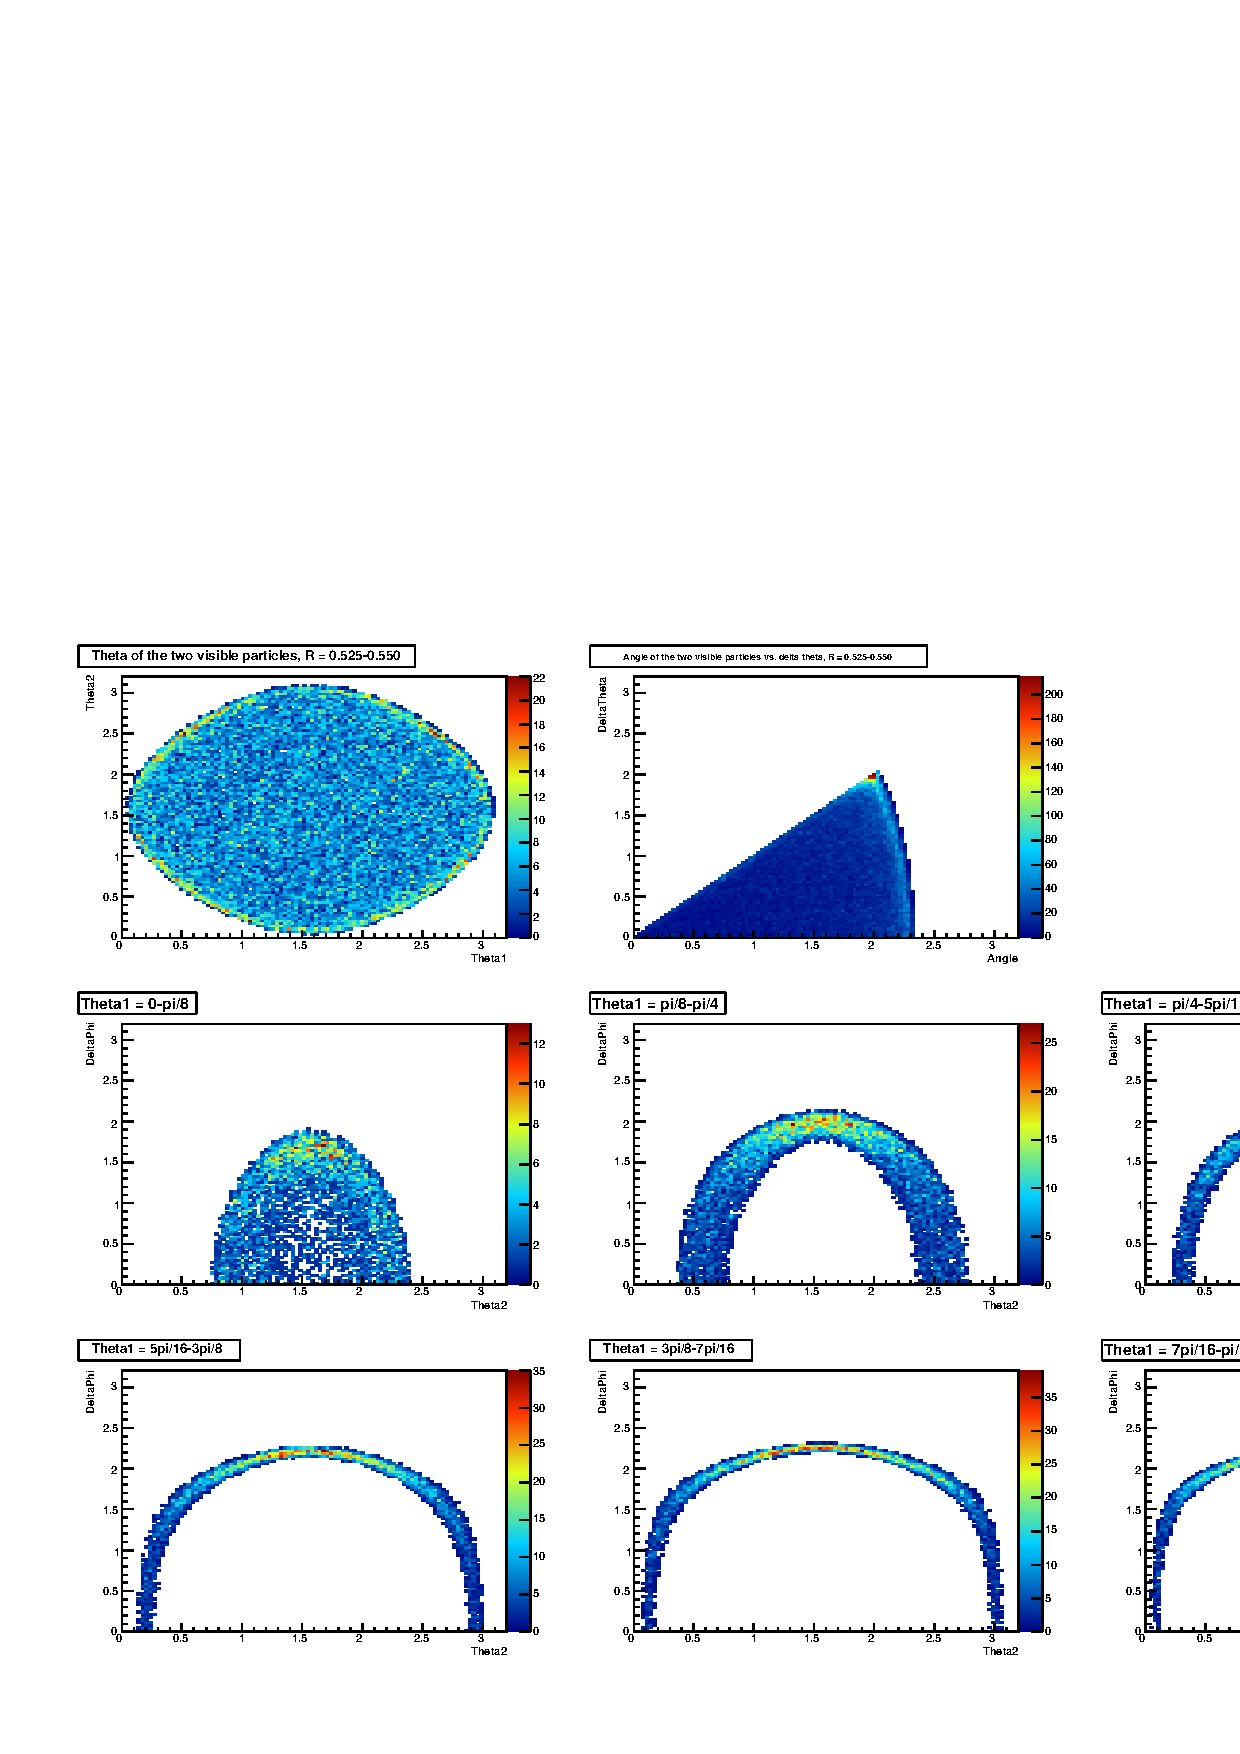
\includegraphics[width=11cm]{Figures/MRToy12_RPhaseSpace_LargeR}
   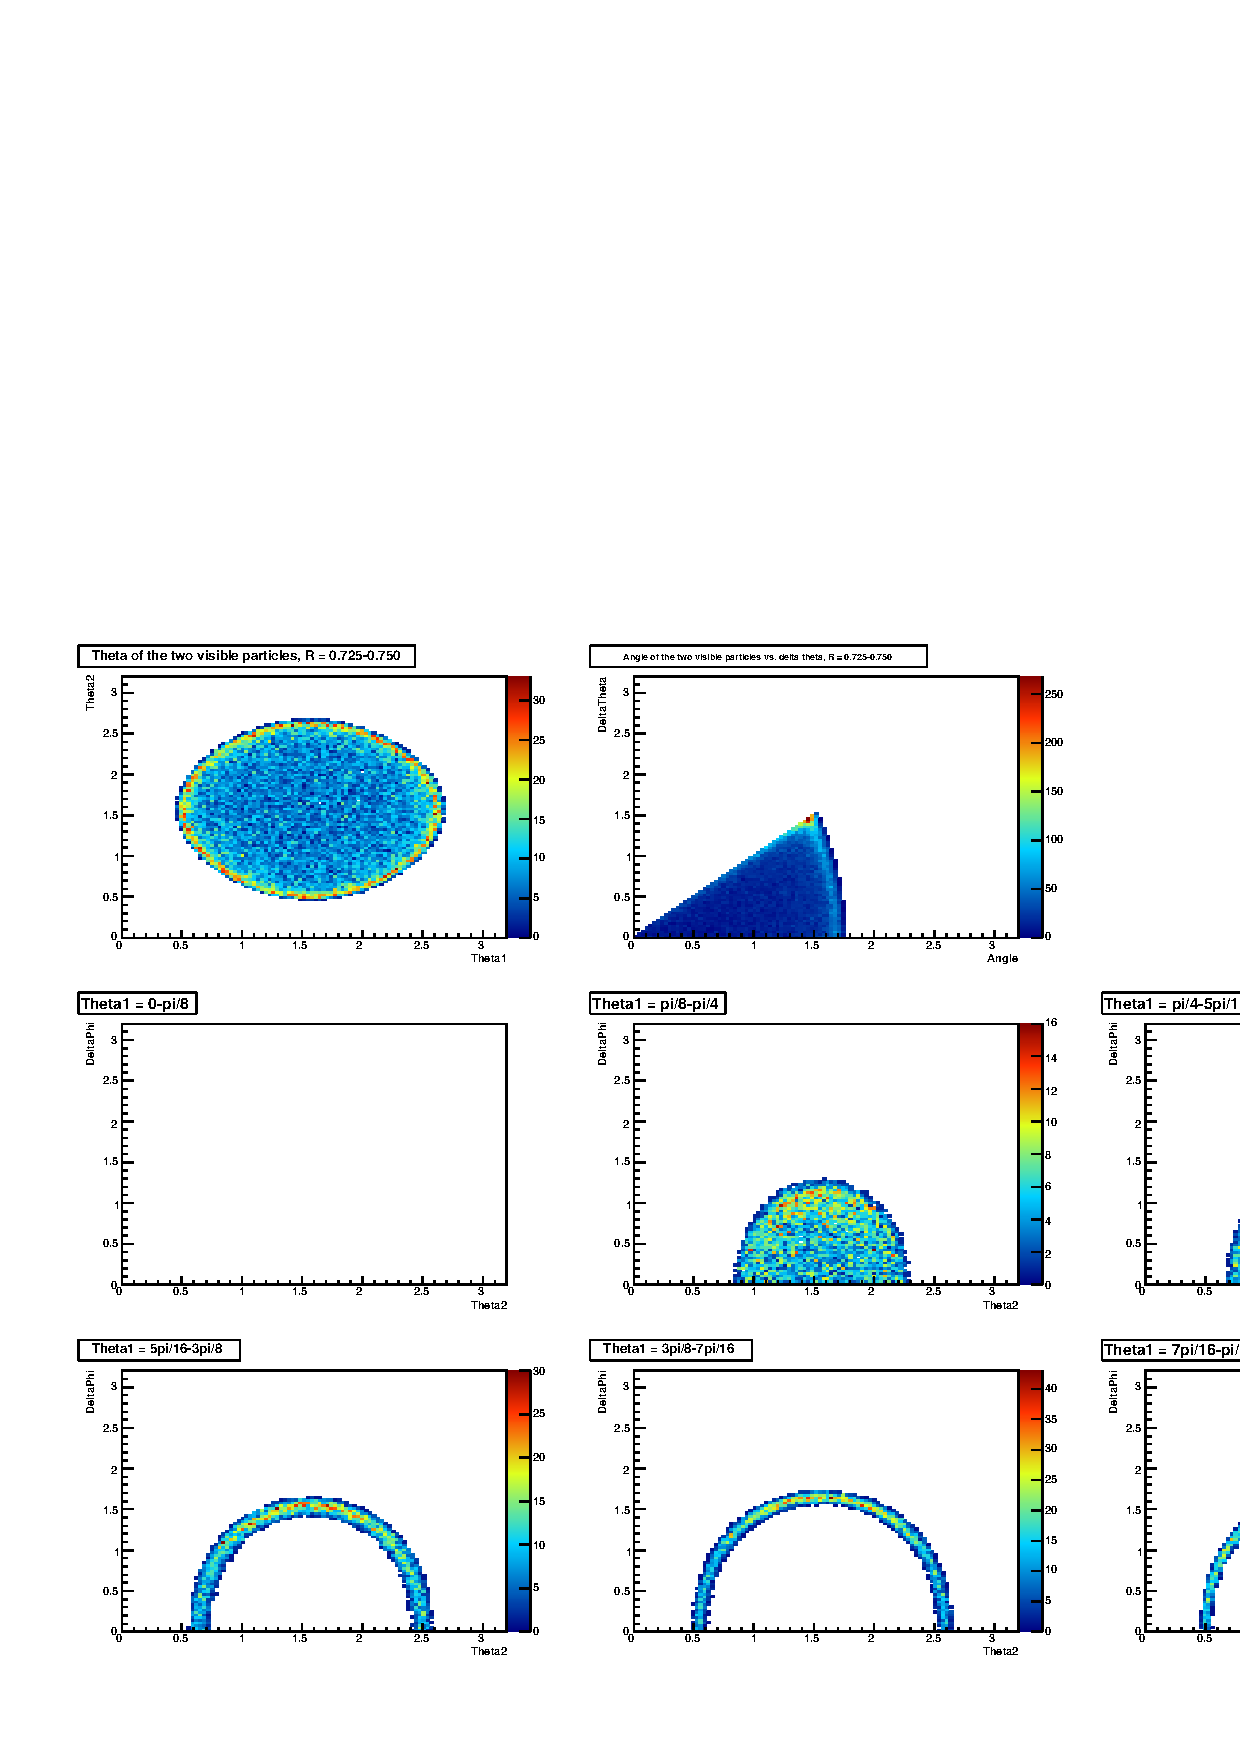
\includegraphics[width=11cm]{Figures/MRToy12_RPhaseSpace_HugeR}
   \caption{MRToy 12, mapping out phase space for different R value, raw distribution.
      The R values plotted are 0.125-0.150 for upper left, 0.325-0.350 upper right, 0.525-0.550 lower left, 0.725-0.750 lower right.
      If this looks mystic, don't worry.  There is a summary sketch.}
   \label{Figure_MRToy12_Raw}
\end{figure}
\end{landscape}


\begin{figure}[htbp]
   \centering
   \fbox{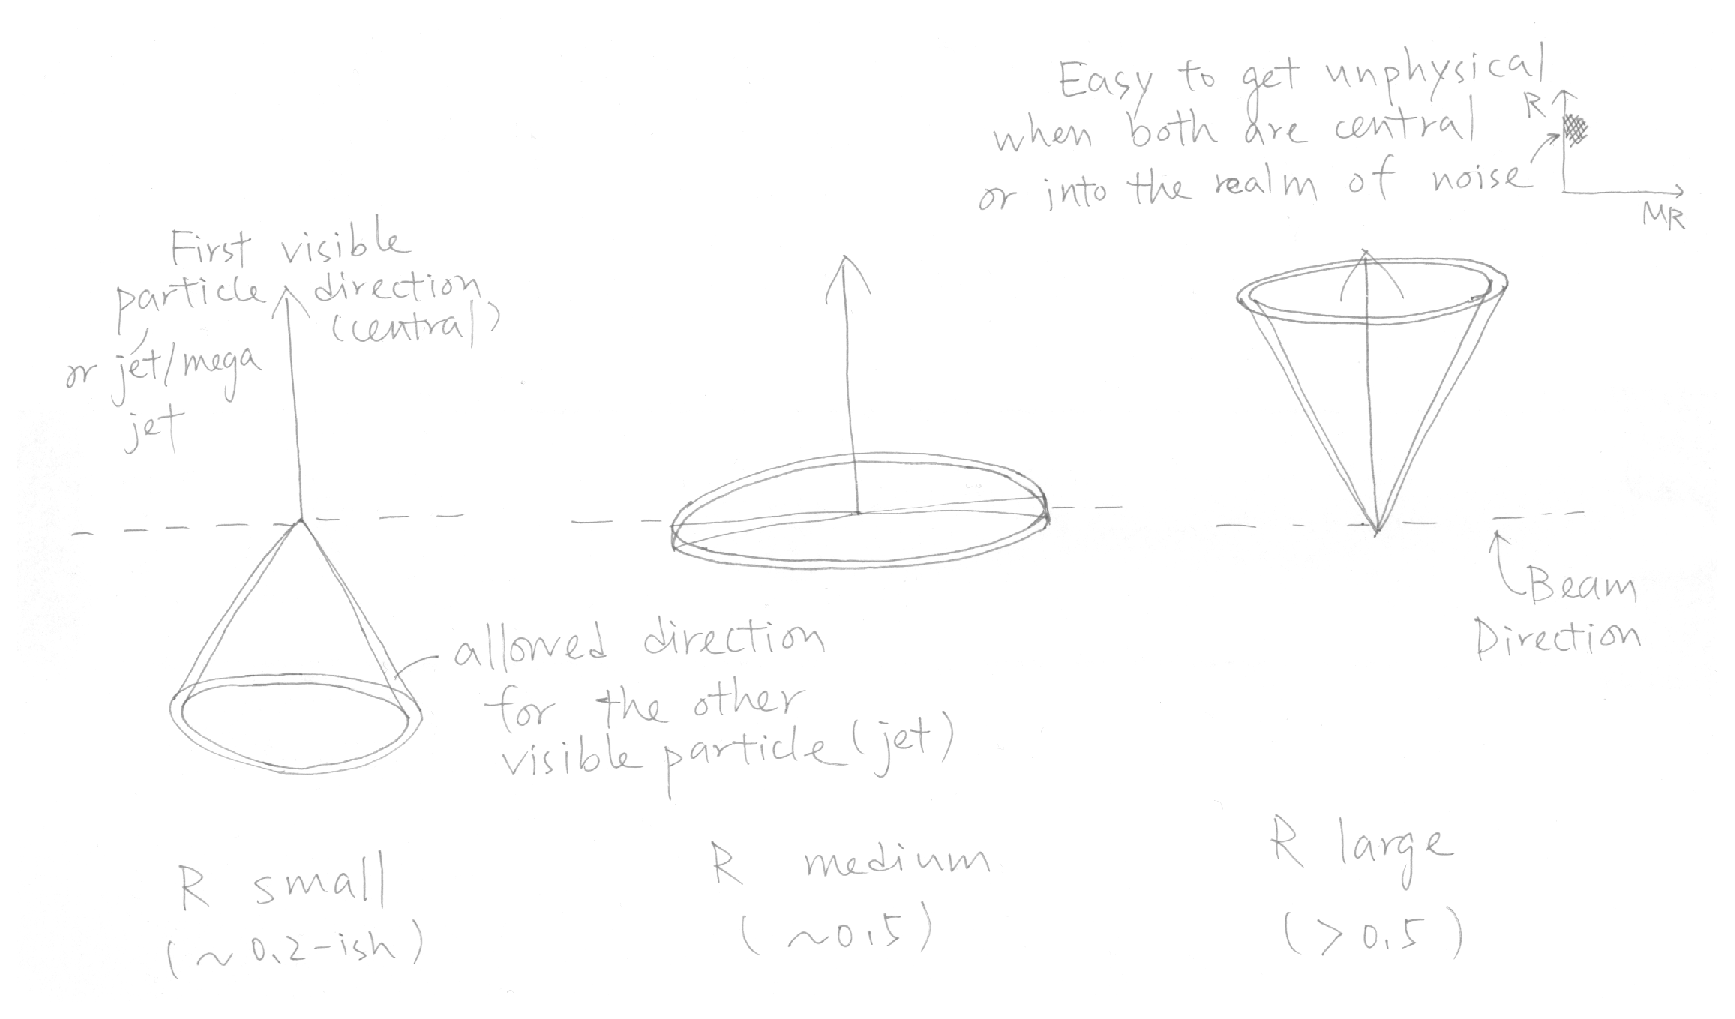
\includegraphics[width=15cm]{Figures/RSketch}}
   \caption{MRToy 12, summary sketch when one of the visible particle is central.  If the first one is forward, the allowed region for the other particle
   is slanted, but the general picture is similar.}
   \label{Figure_MRToy12_Summary}
\end{figure}


\subsection{MRToy 5-2, mapping out angular distributions in each part of $R-M_R$ plane}

Referring to MRToy 5 as shown below, which investigates how things will change in the presence of non-negligible transverse boost of the whole system,
there are some strange features.  In the end it was never clear why there are this weird feature, but instead we have more insight on what the
allowed phase space looks like in different region in the $R-M_R$ plane.

A few selected regions are shown in figures \ref{Figure_MRToy5_2}.
One immediate observation is that when we go towards upper-right corner in the $R-M_R$ plane, angle between visible particles and invisible particles tend to approach $\pi$.
The visible particles are more central as well.  It's hard to make out of these plots, even though a lot of information is contained.

It's best to visualize using 3D plotting tools (or even interactive histogram!), but I haven't found time to play with it.

\begin{figure}[htbp]
   \centering
   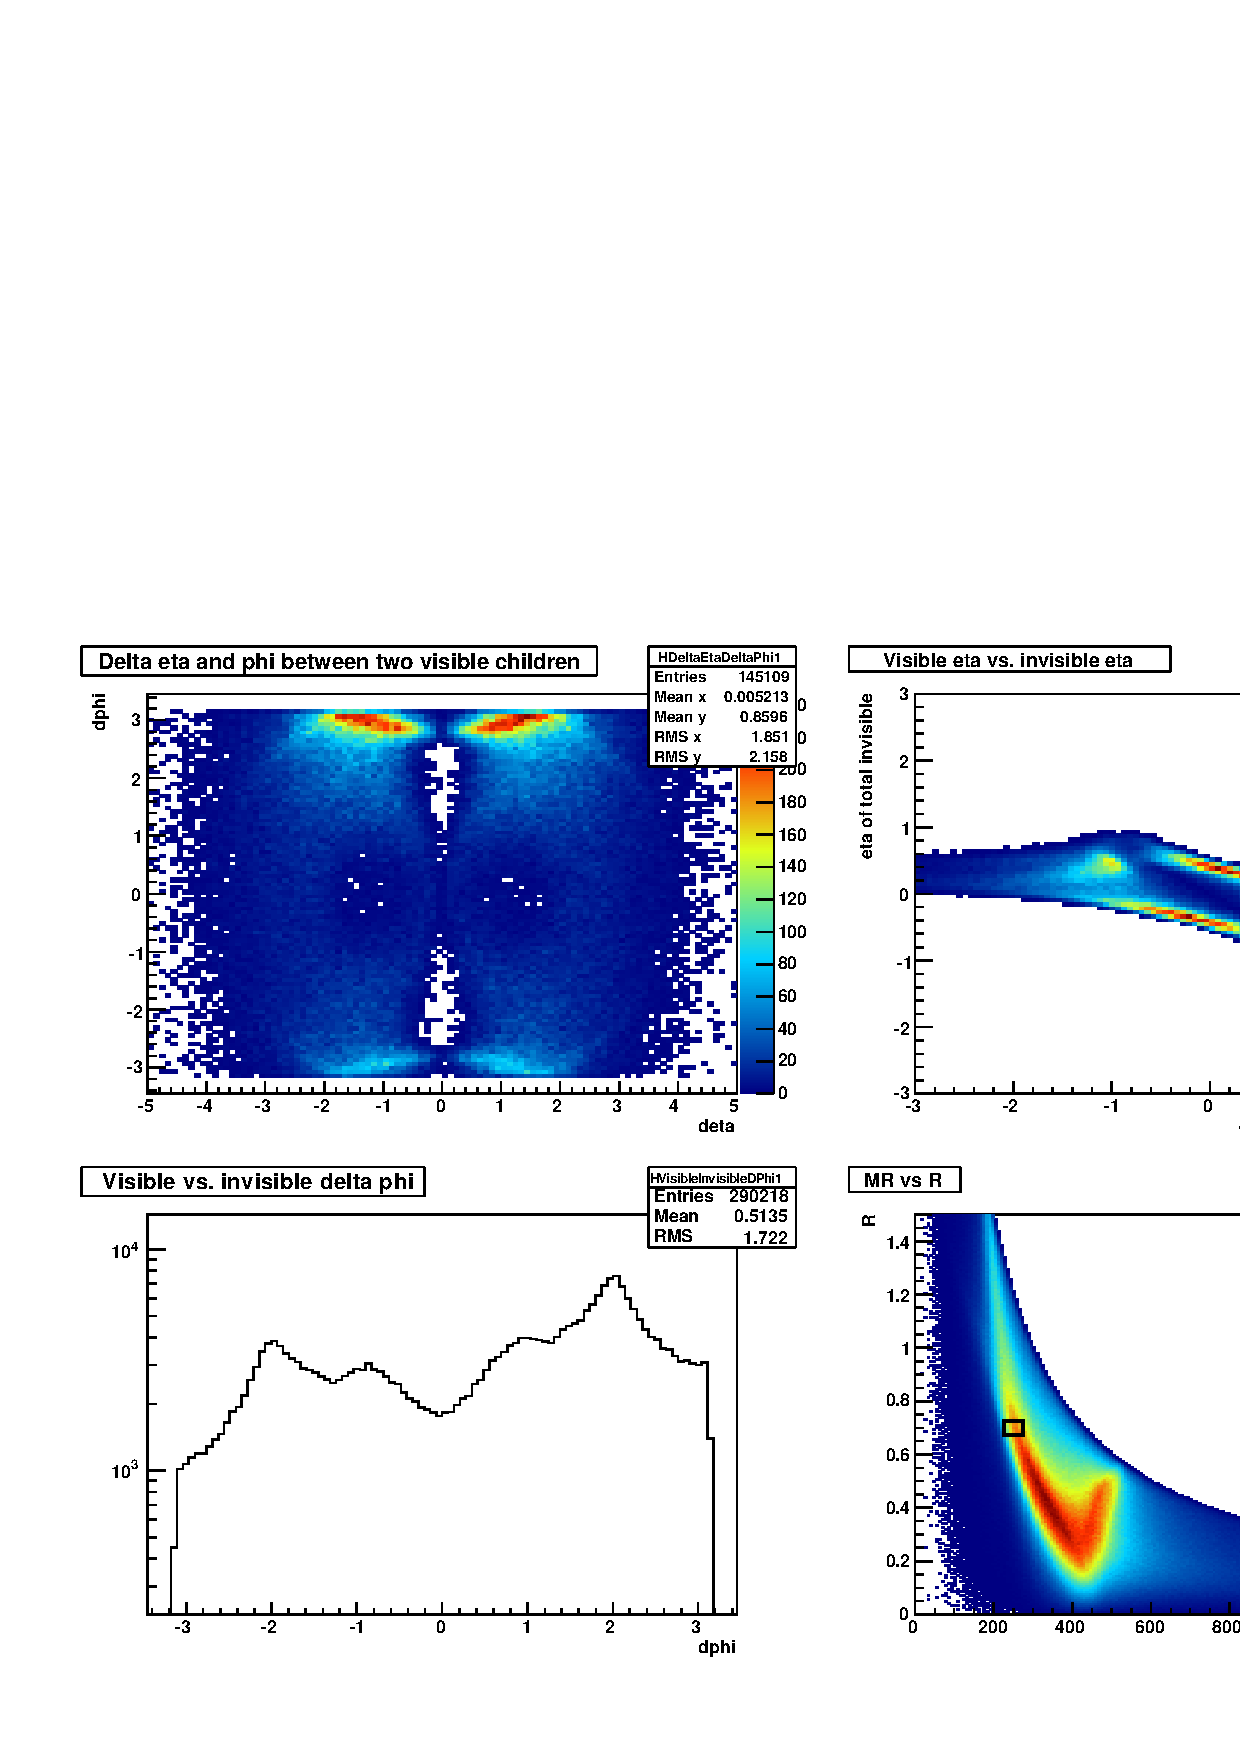
\includegraphics[width=7cm]{Figures/MRToy5_2_Region1}
   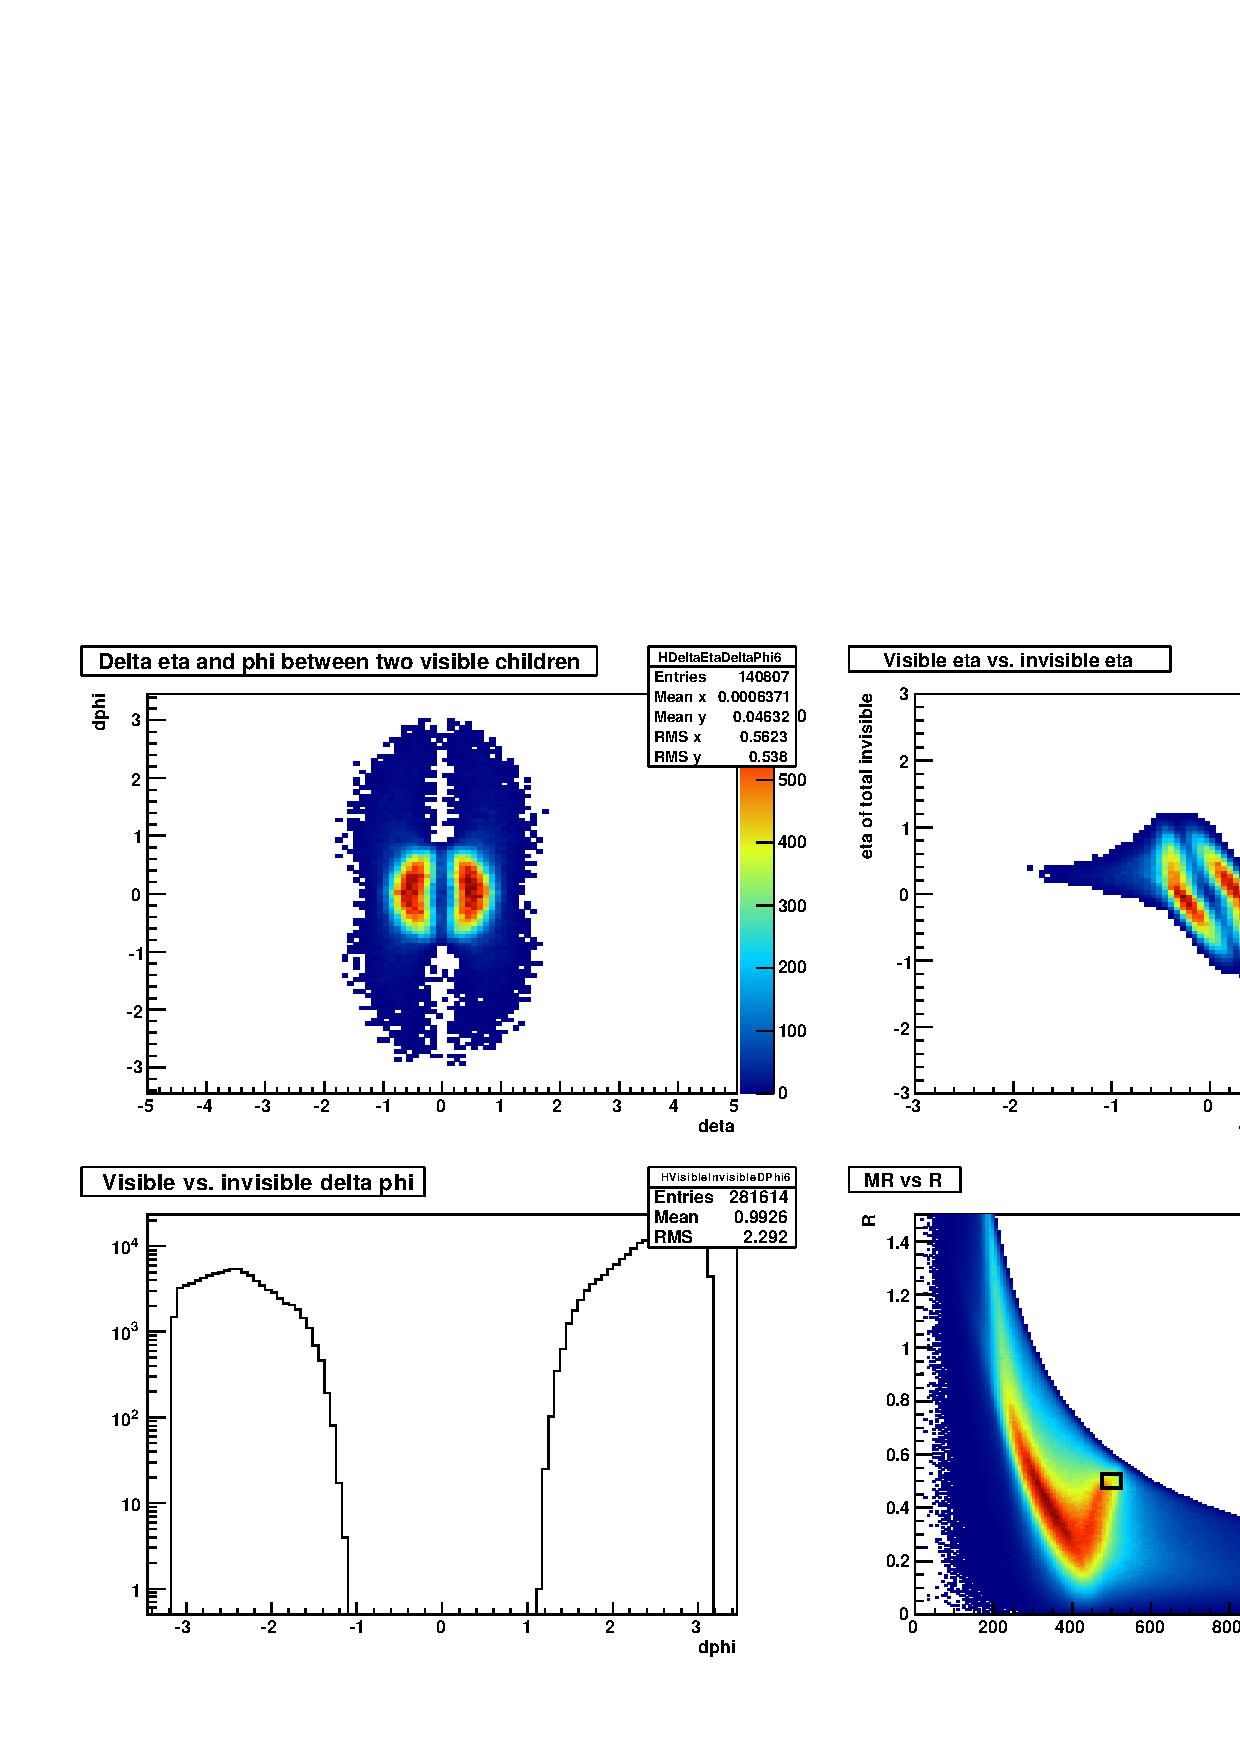
\includegraphics[width=7cm]{Figures/MRToy5_2_Region2}\\
   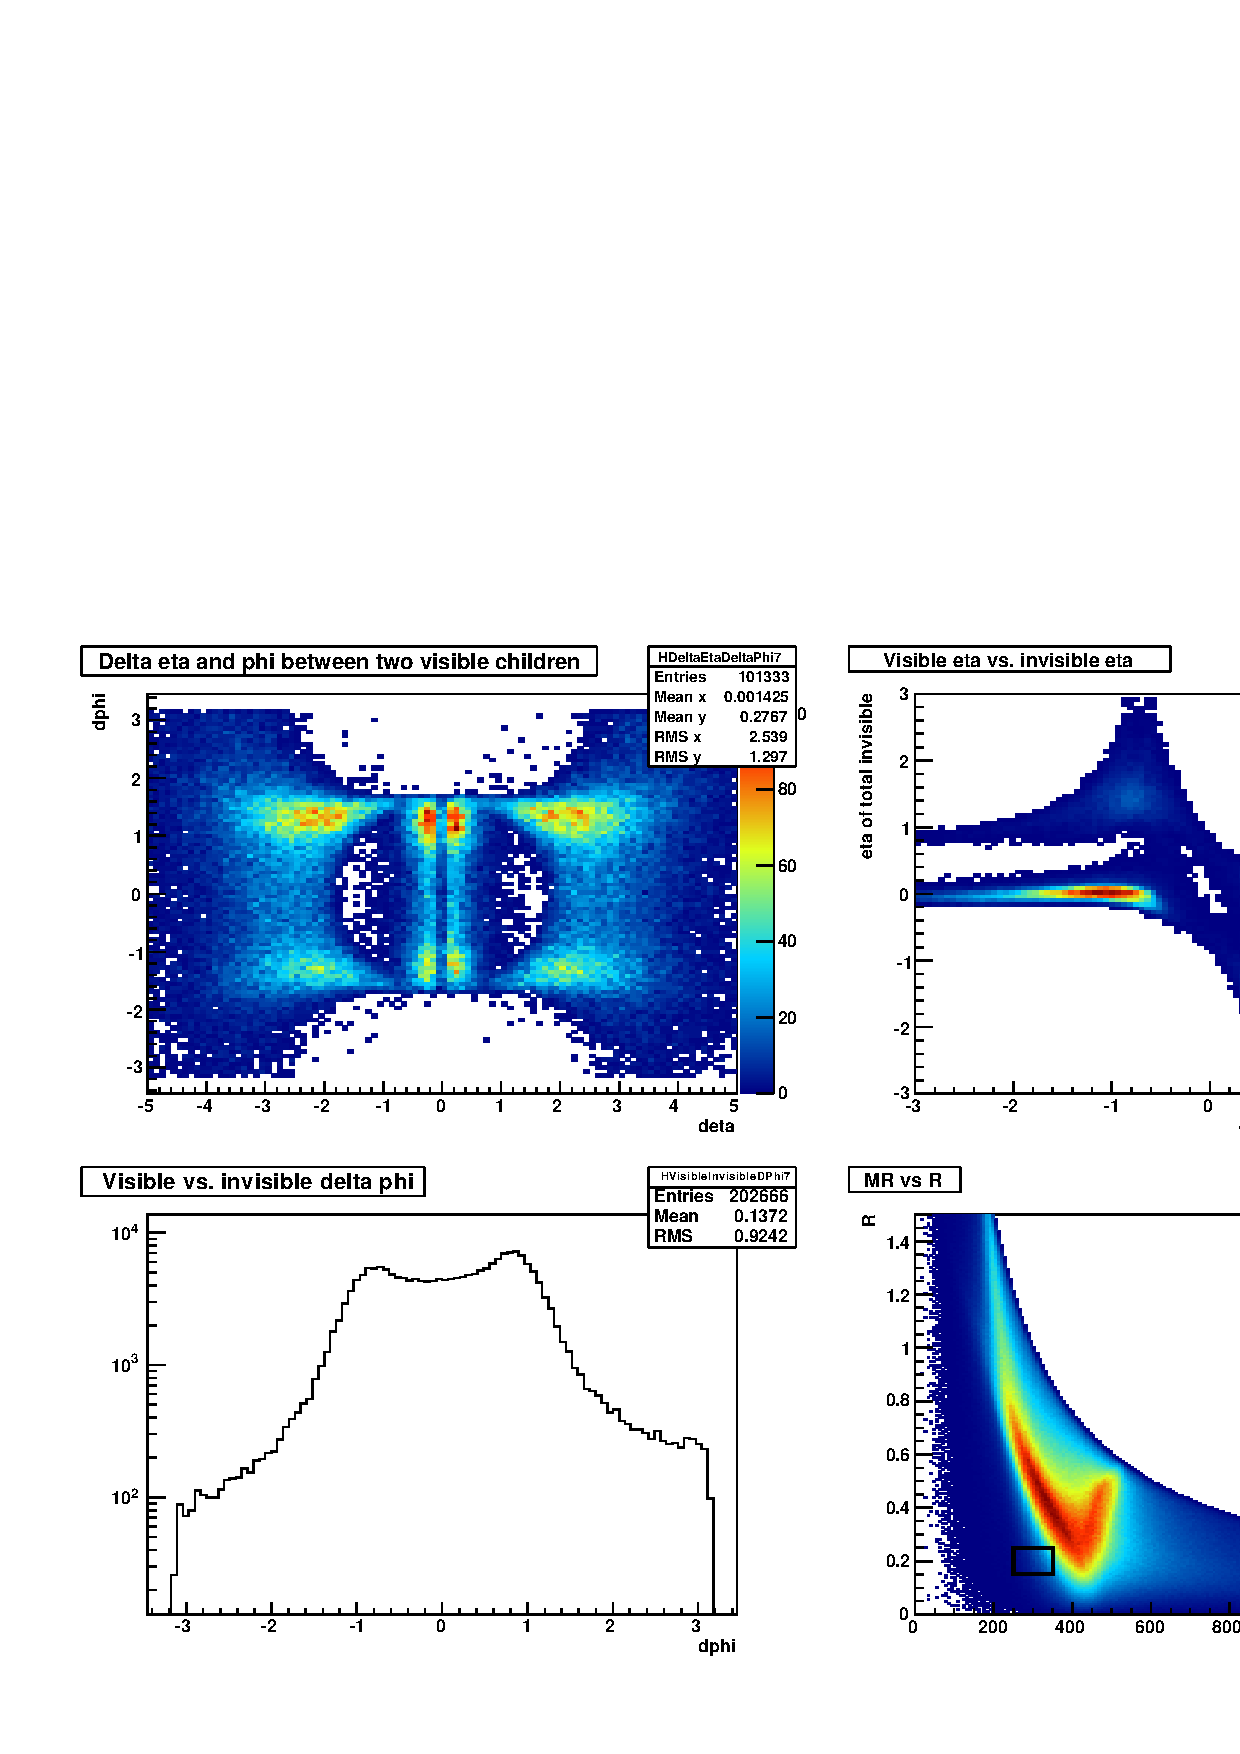
\includegraphics[width=7cm]{Figures/MRToy5_2_Region3}
   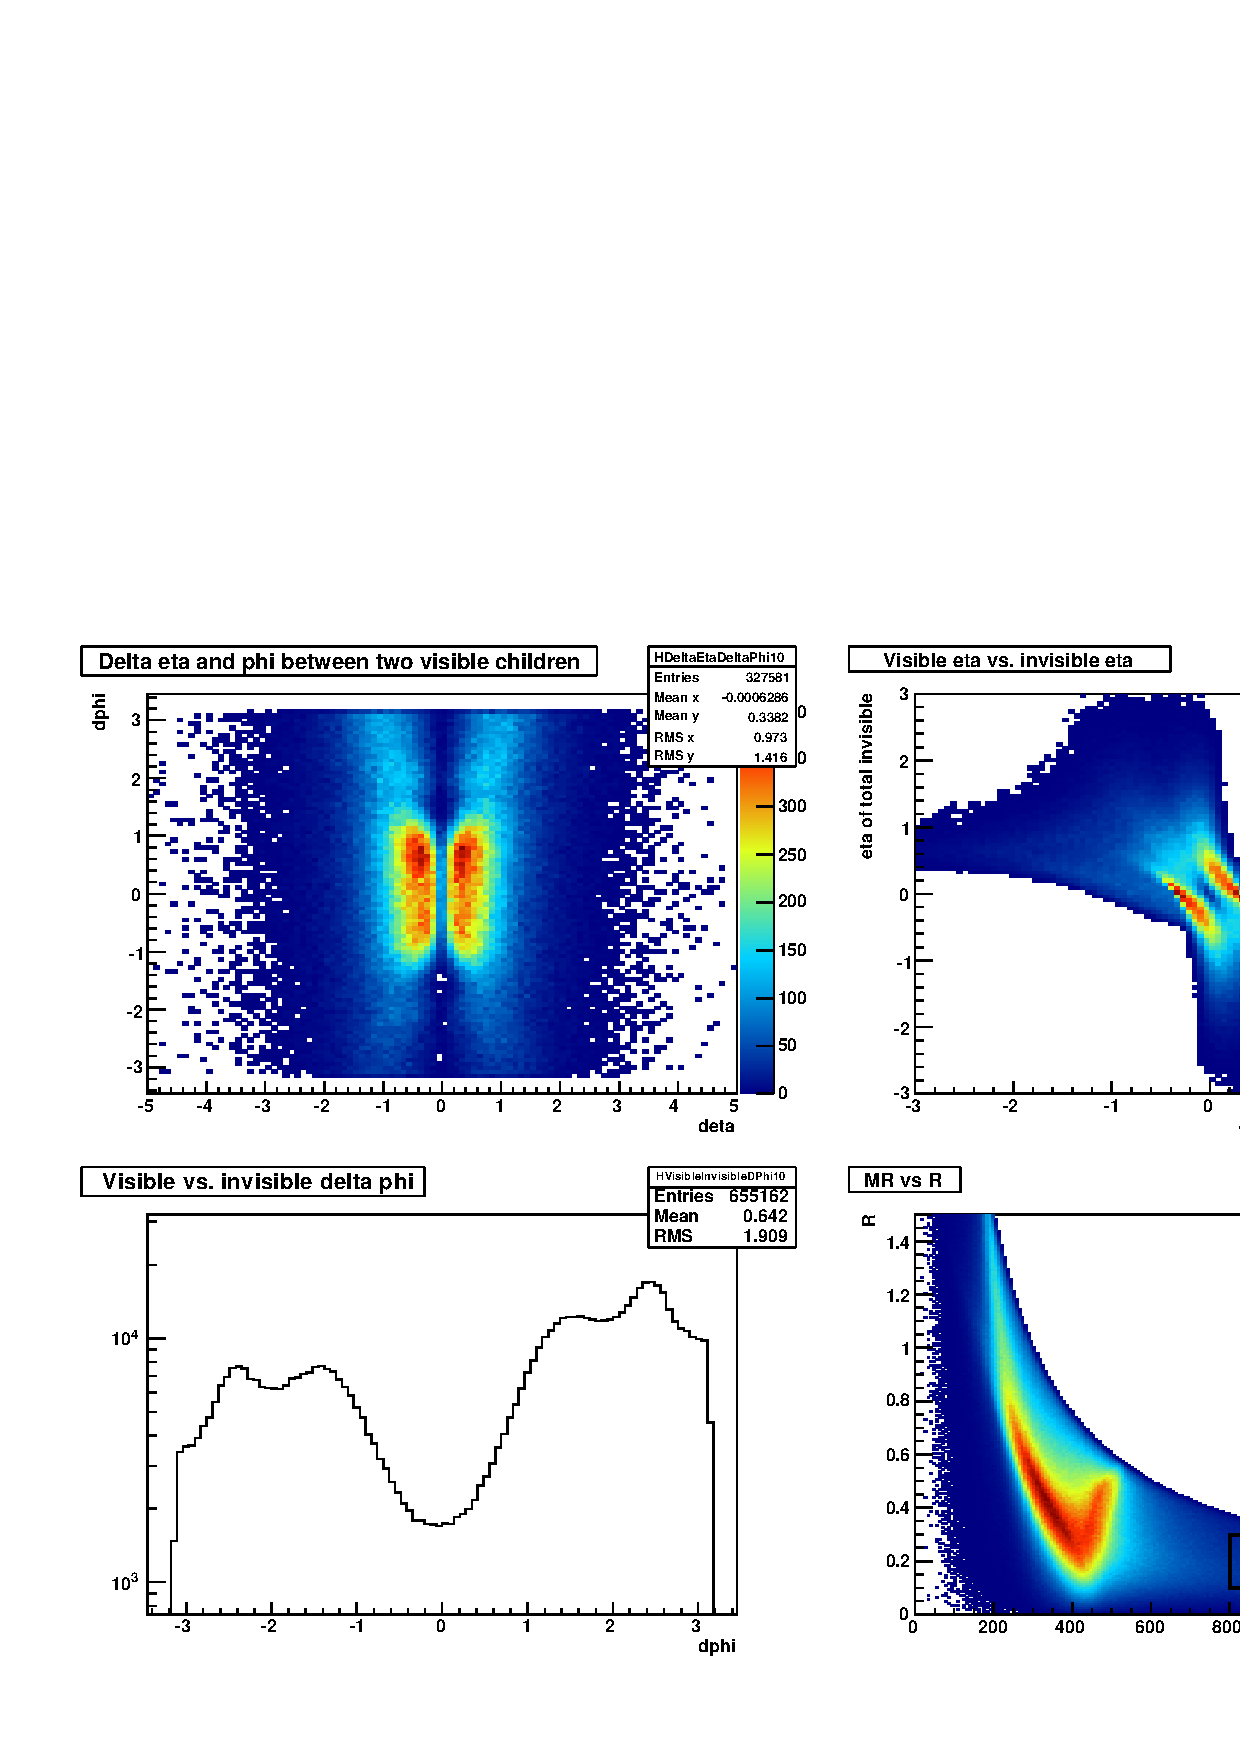
\includegraphics[width=7cm]{Figures/MRToy5_2_Region4}
   \caption{MRToy 5-2, angular distributions from different regions.}
   \label{Figure_MRToy5_2}
\end{figure}



\subsection{MRToy 11.  Pythia 8 generated events, hard process only.}

Let's see the effect of various processes on $M_R$ and $R$.  The three toggle-able things are multiple interaction, initial state radiation and final state radiation.
The comparison is in figure \ref{Figure_MRToy11}.  The variables are constructed using the ``final'' b quark, so in case of multiple interaction and initial state radiation we don't see much change.
However in final state radiation since part of the energy is radiated away, we see that $M_R$ is decreasing.
Even though the final state radiation is erroneous, at least the qualitative statement is correct.

On the other hand, if we group things into jets and then hemispheres, as shown in figure \ref{Figure_MRToy11_Hemisphere}, the picture is slightly different.
For multiple interaction not much change is seen, since the extra jets are seen to be soft, at least in transverse momentum.
An example diagram is shown in figure \ref{Figure_Pythia8MIExample}.
In the case of ISR, since any energy is seen as extra with respect to the hard process, $M_R$ increases.
When it is FSR only, nothing changes.  Energy might get reshuffled between two hemispheres (which subsequently changes $M_R$ a bit), but we get back what is in the original hard process by grouping things into hemispheres.

\begin{figure}[htbp]
   \centering
   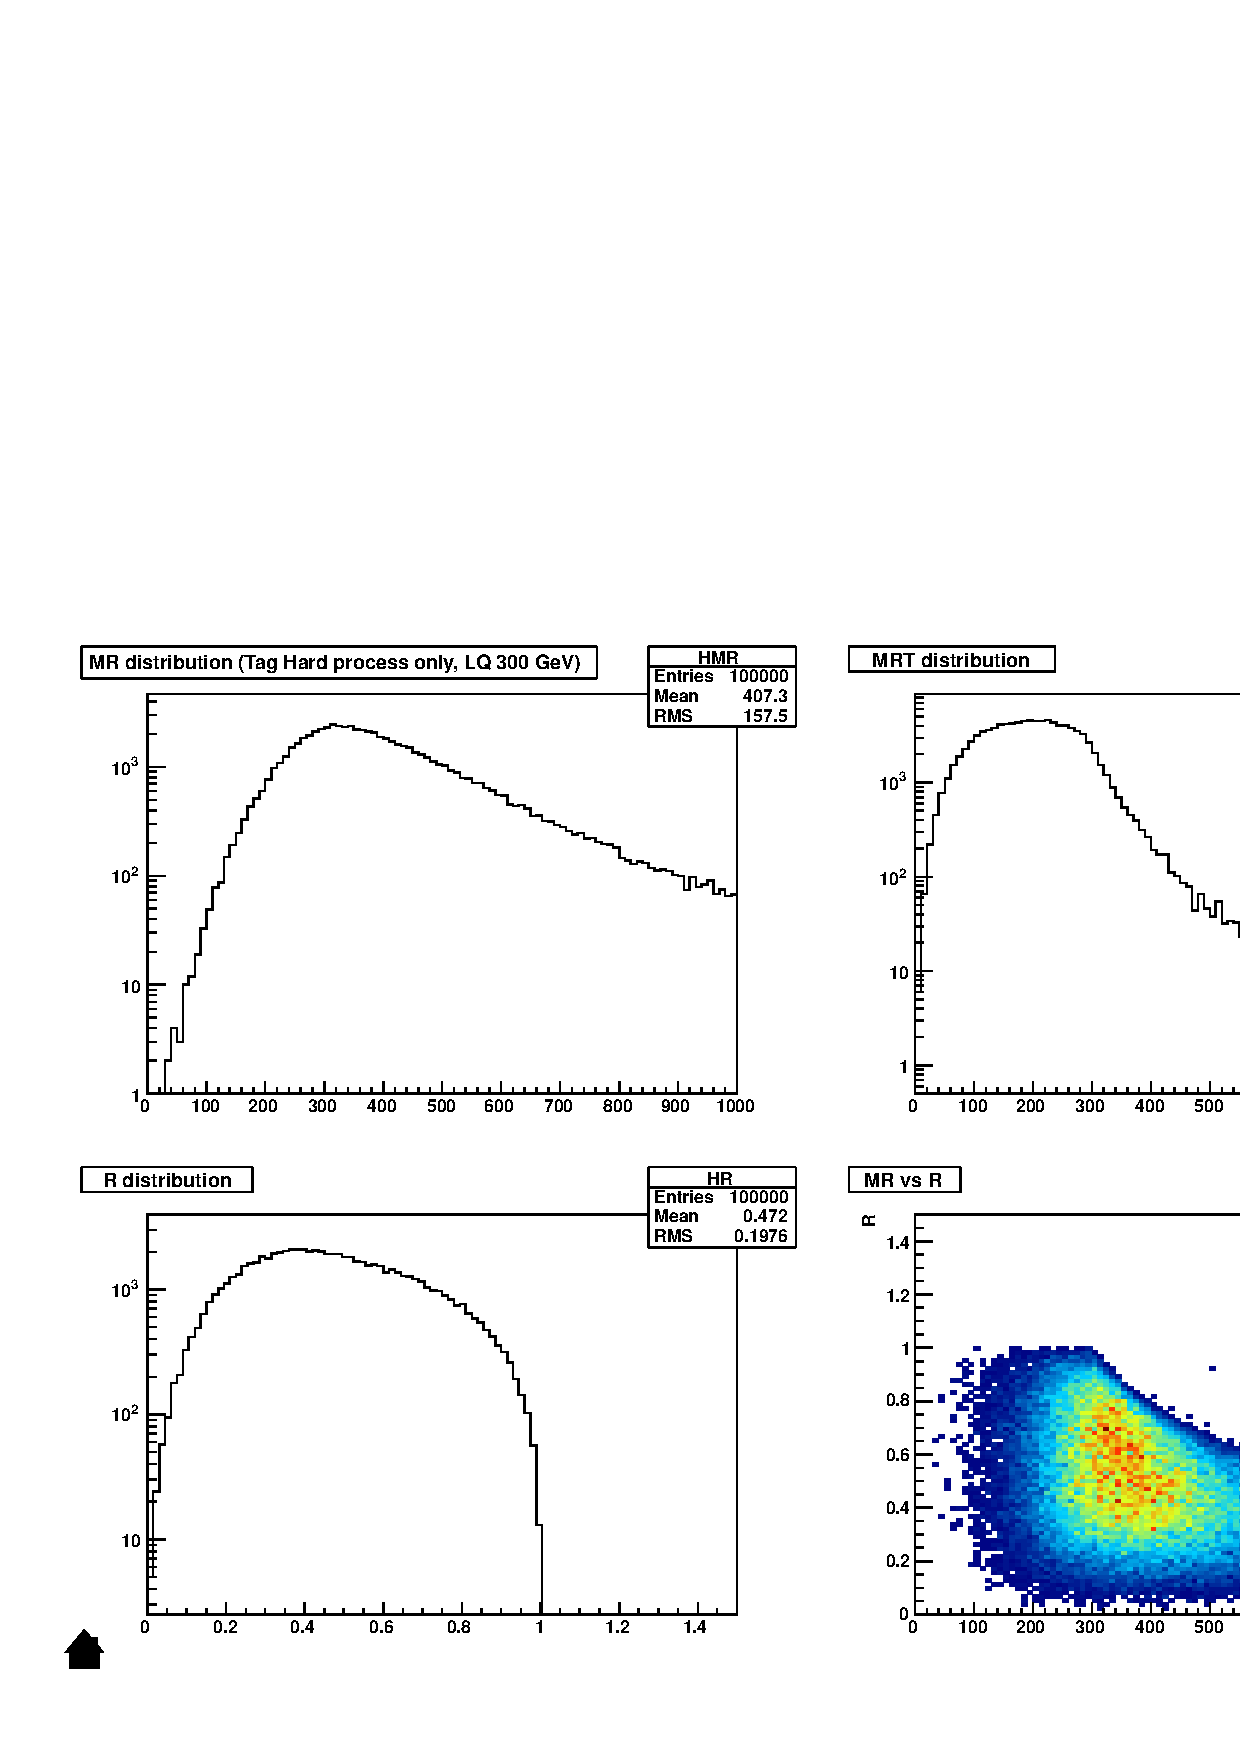
\includegraphics[width=7cm]{Figures/MRToy11_Nothing}
   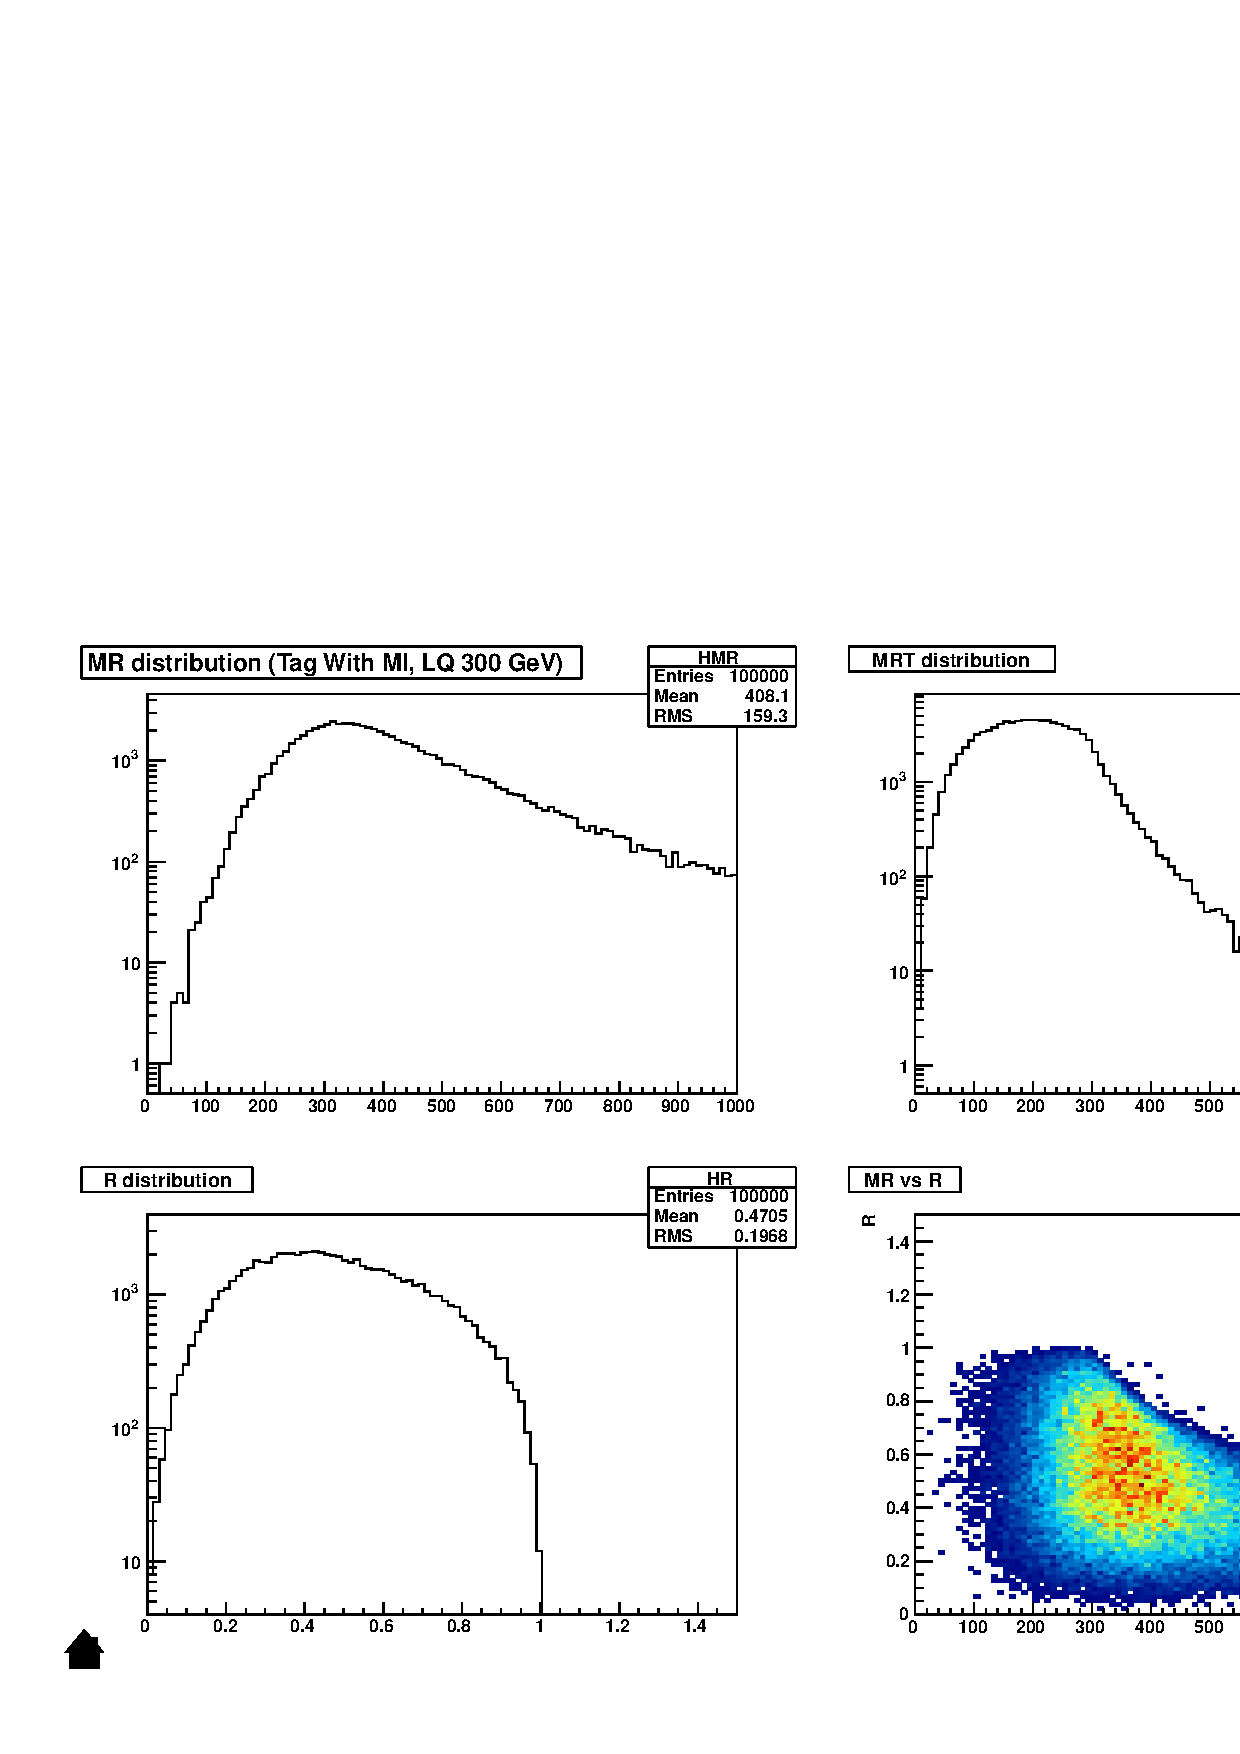
\includegraphics[width=7cm]{Figures/MRToy11_MI}\\
   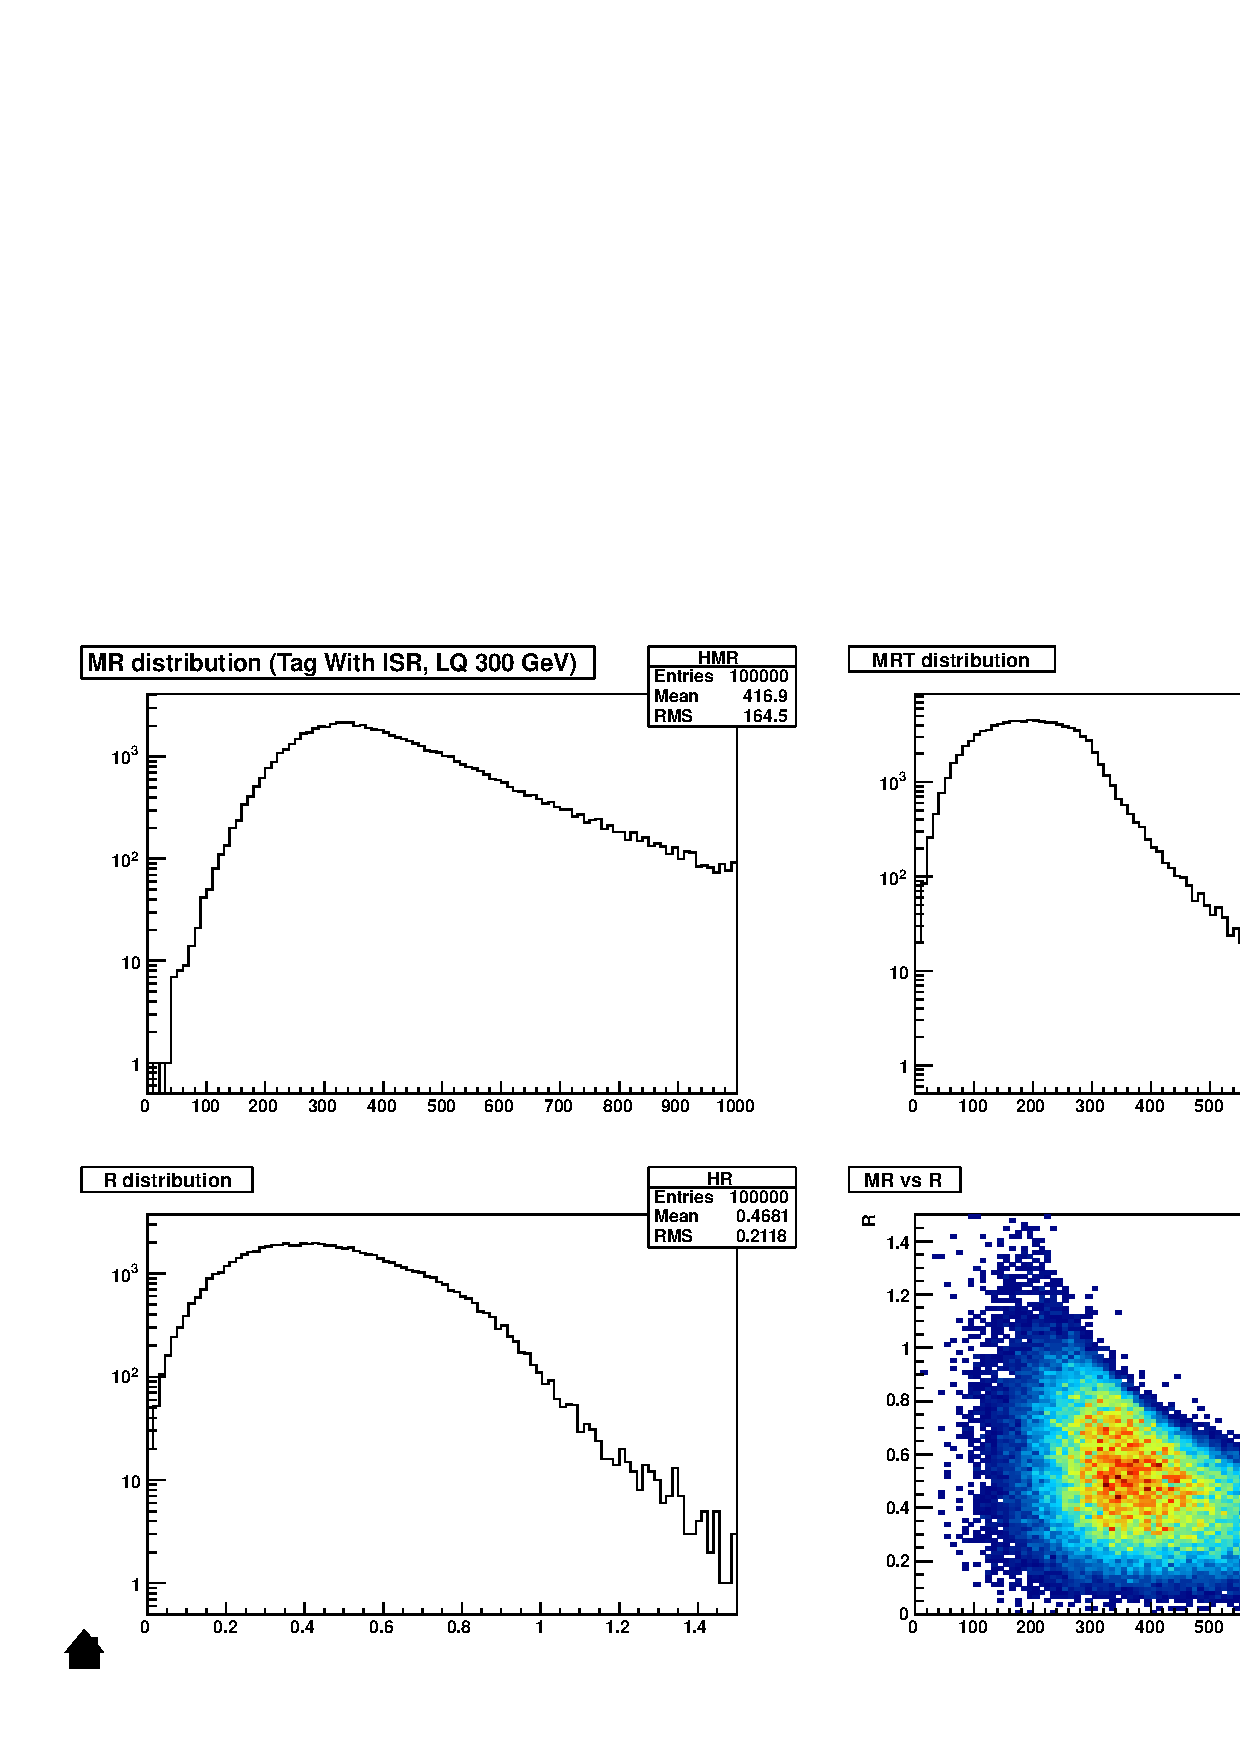
\includegraphics[width=7cm]{Figures/MRToy11_ISR}
   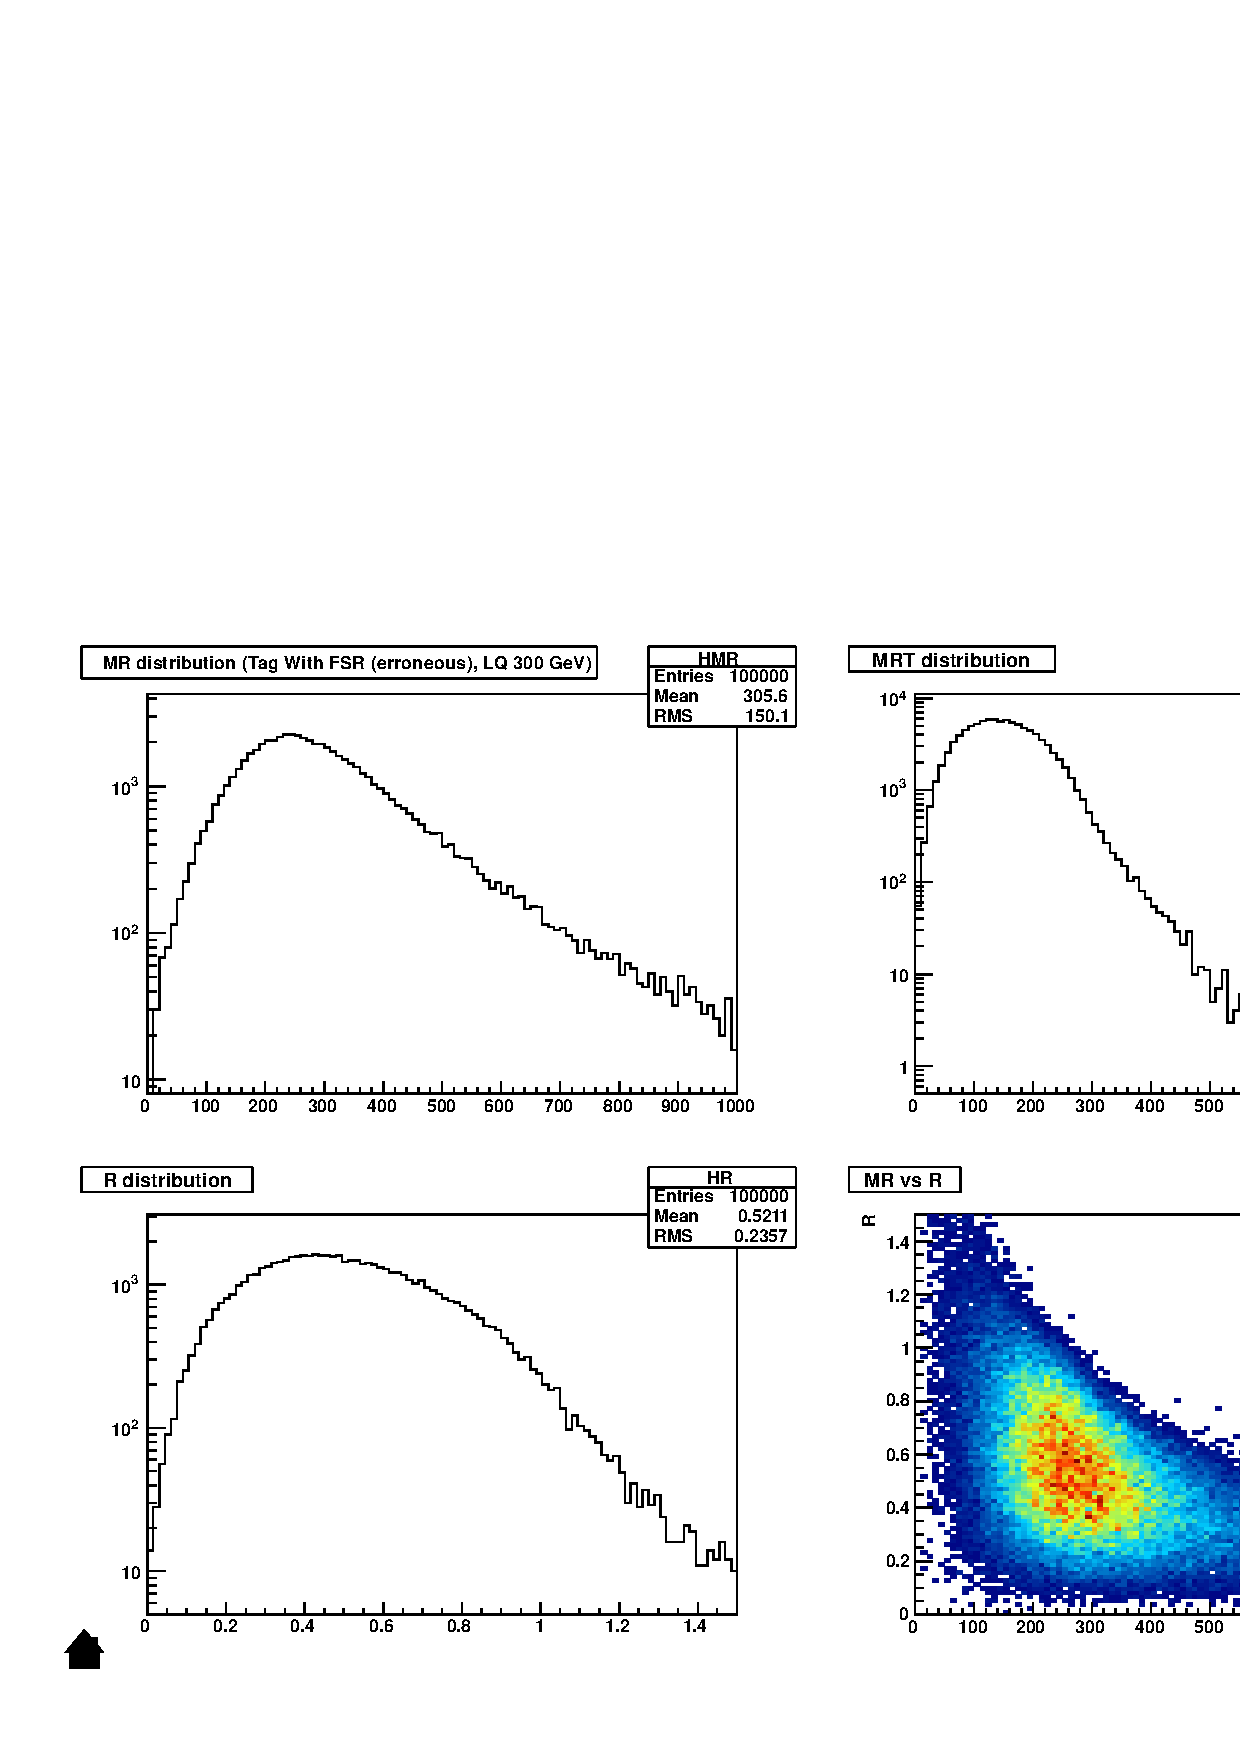
\includegraphics[width=7cm]{Figures/MRToy11_FSR}
   \caption{Look at pythia8-generated LQ sample before hadronization step, switching on/off different components.  Upper left: hard process only.  Upper right: hard process + multiple interaction.
   Lower left: hard process + ISR.  Lower right: hard process + FSR (errorneous).  Variables constructed by the b's.}
   \label{Figure_MRToy11}
\end{figure}

\begin{figure}[htbp]
   \centering
   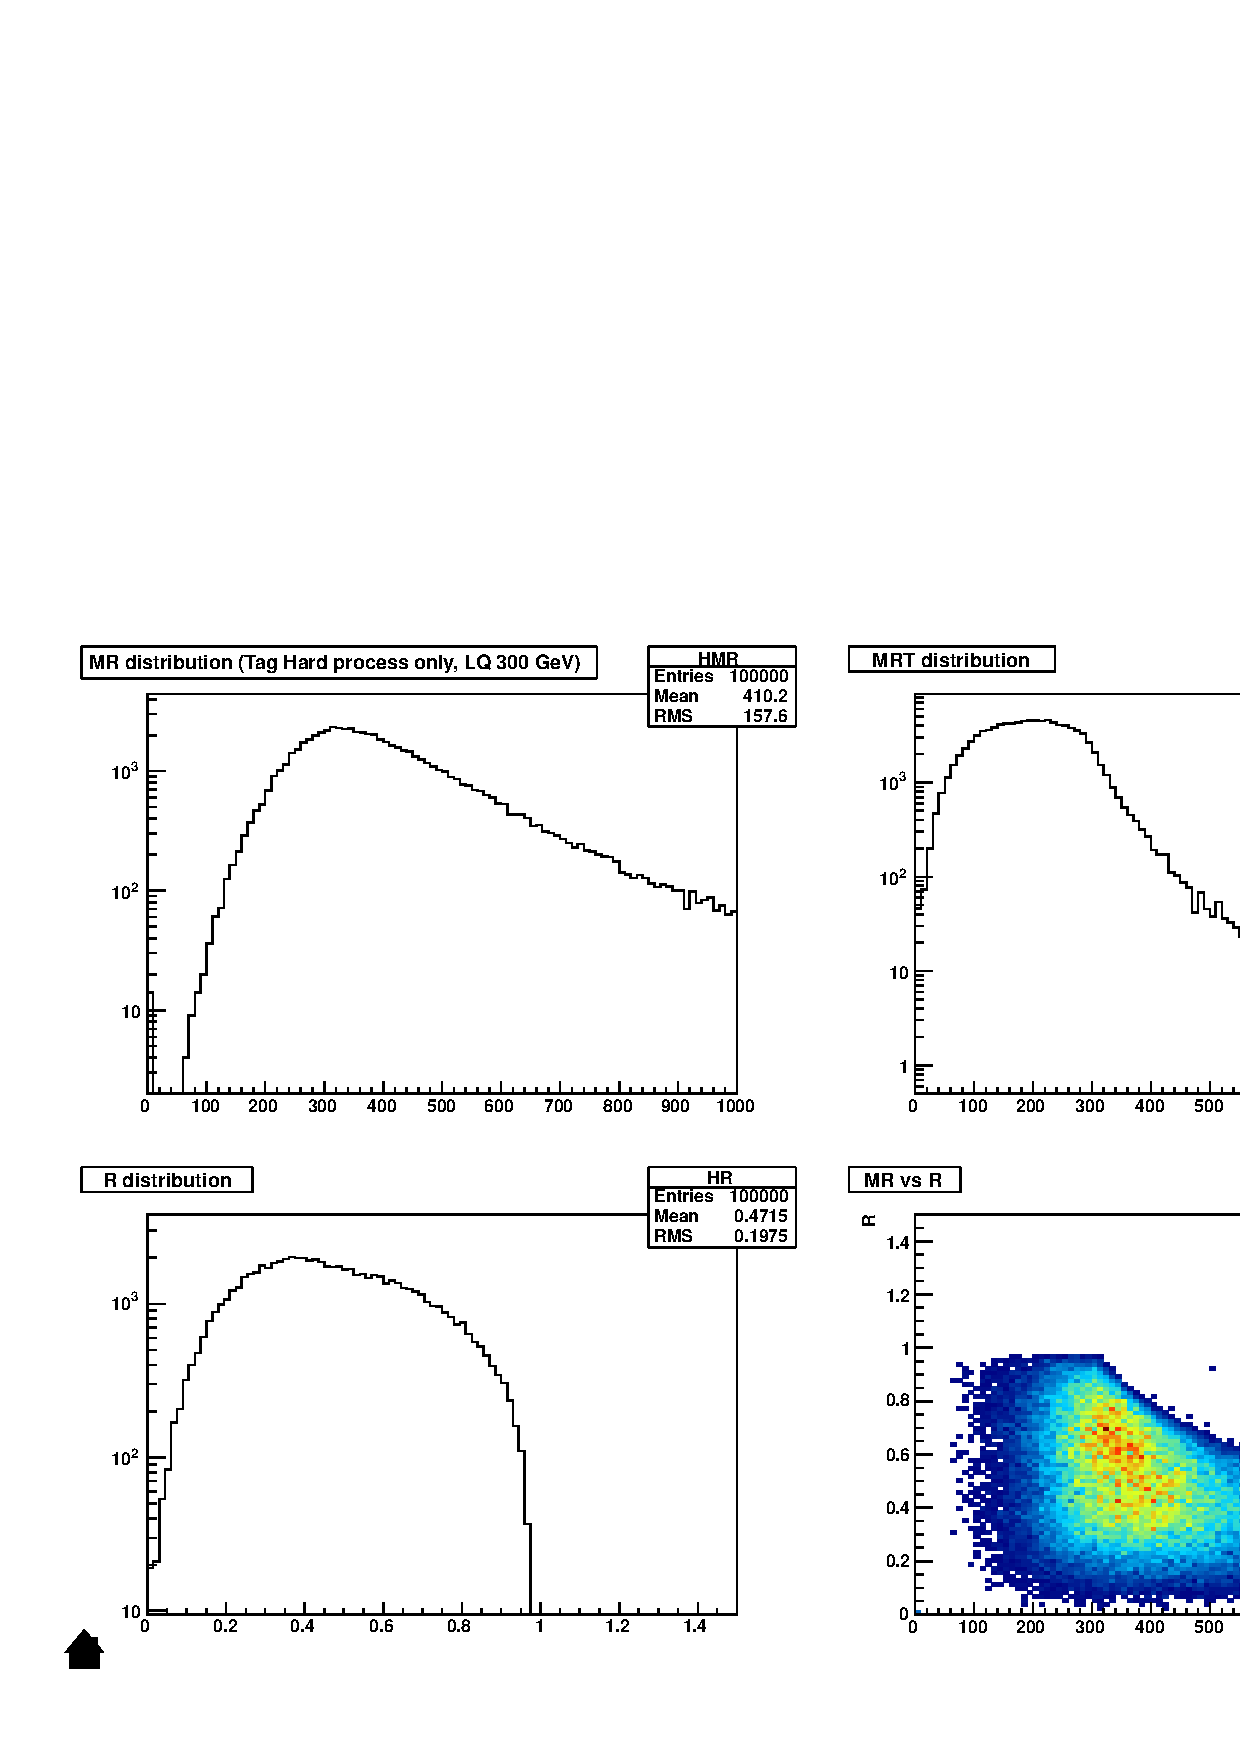
\includegraphics[width=7cm]{Figures/MRToy11_Nothing_Hemisphere}
   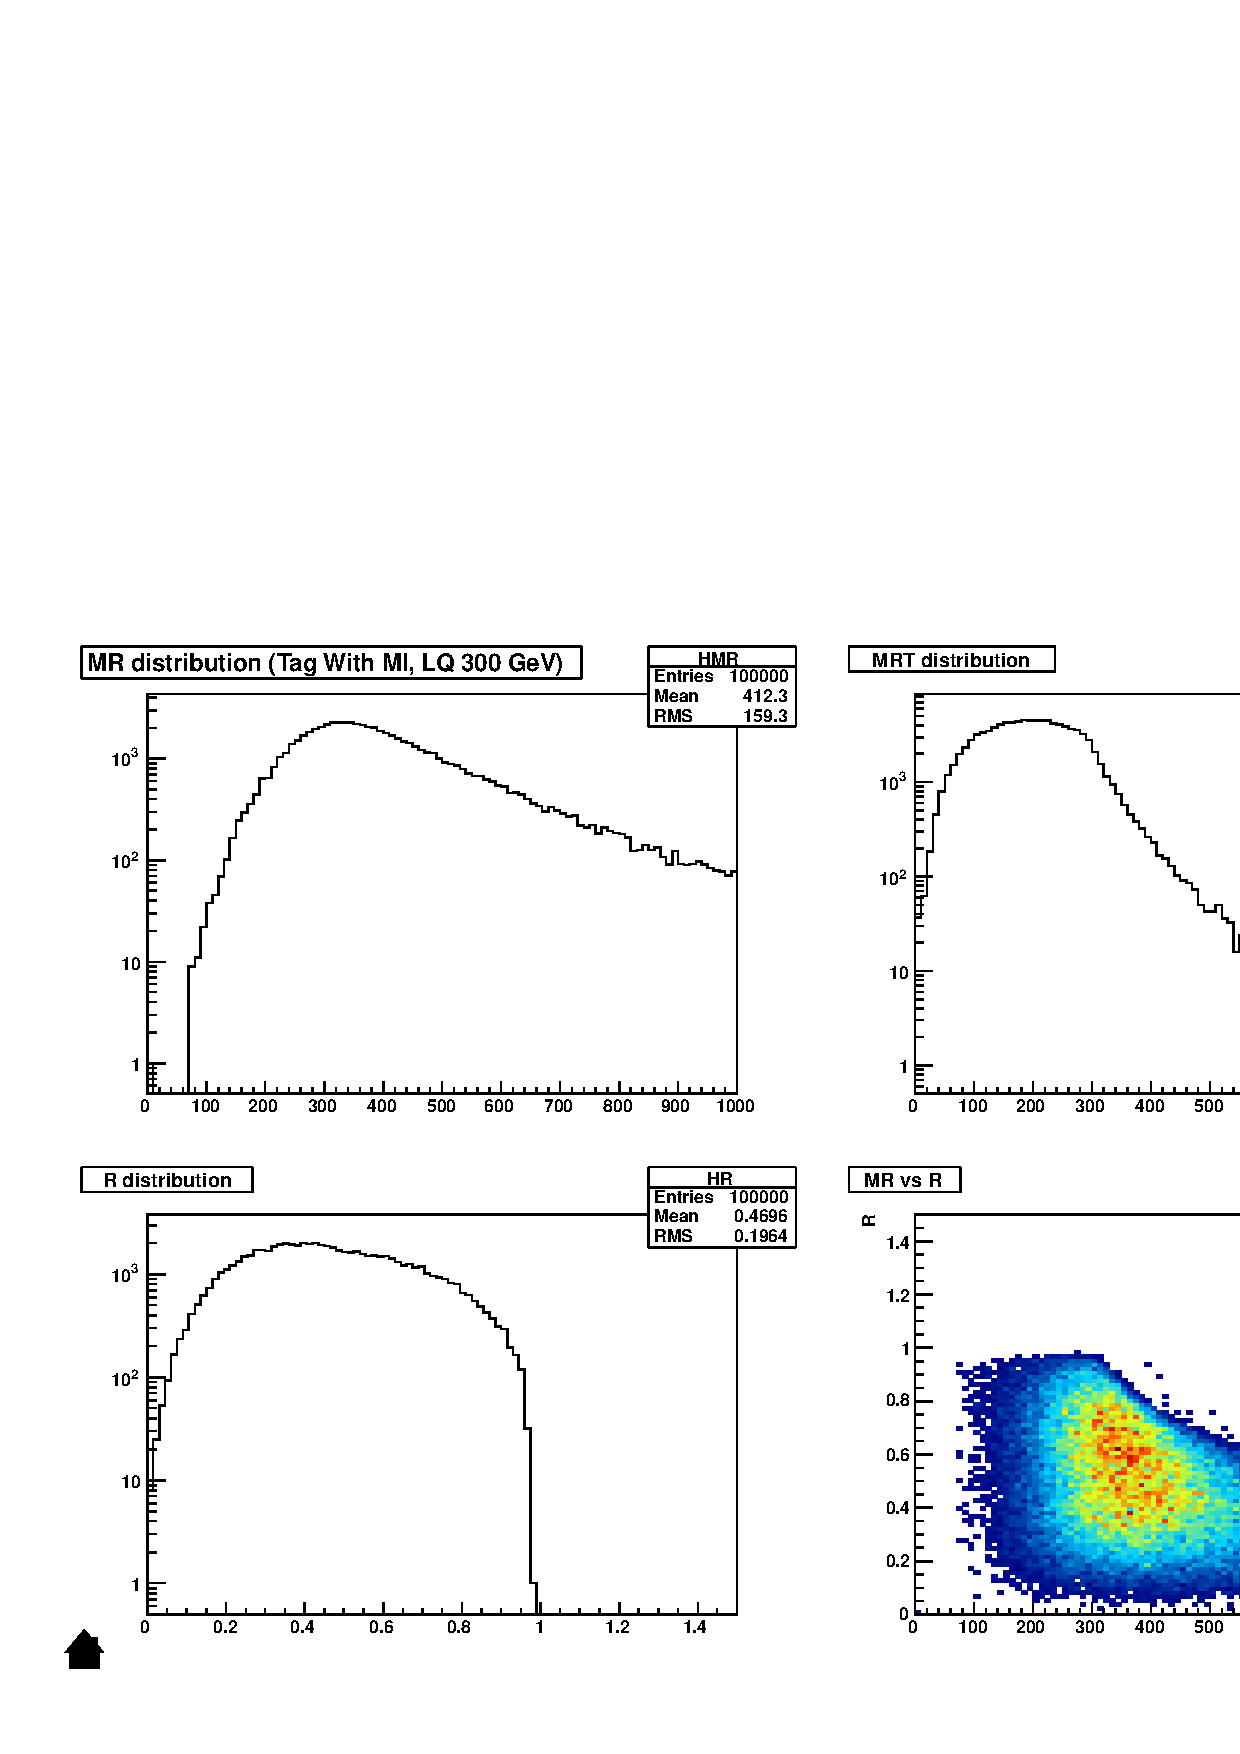
\includegraphics[width=7cm]{Figures/MRToy11_MI_Hemisphere}\\
   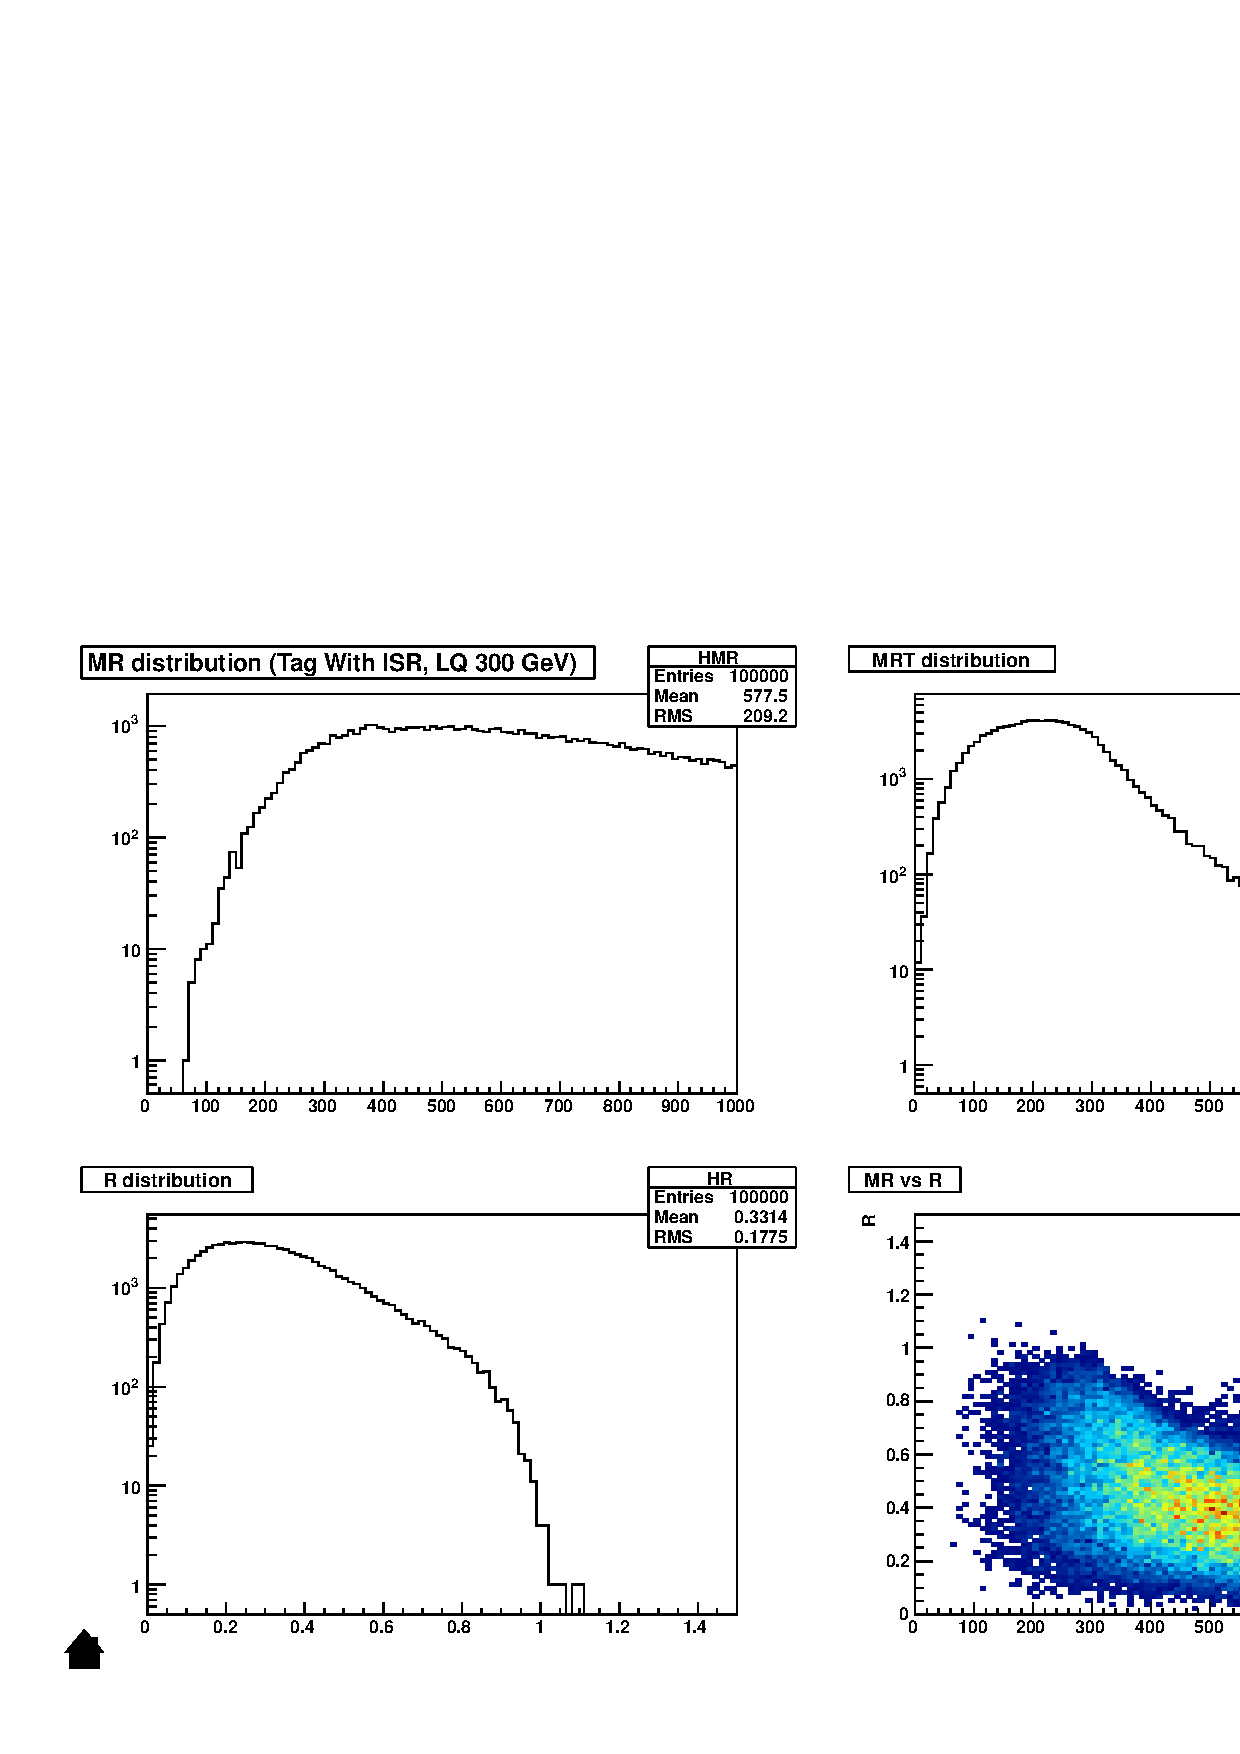
\includegraphics[width=7cm]{Figures/MRToy11_ISR_Hemisphere}
   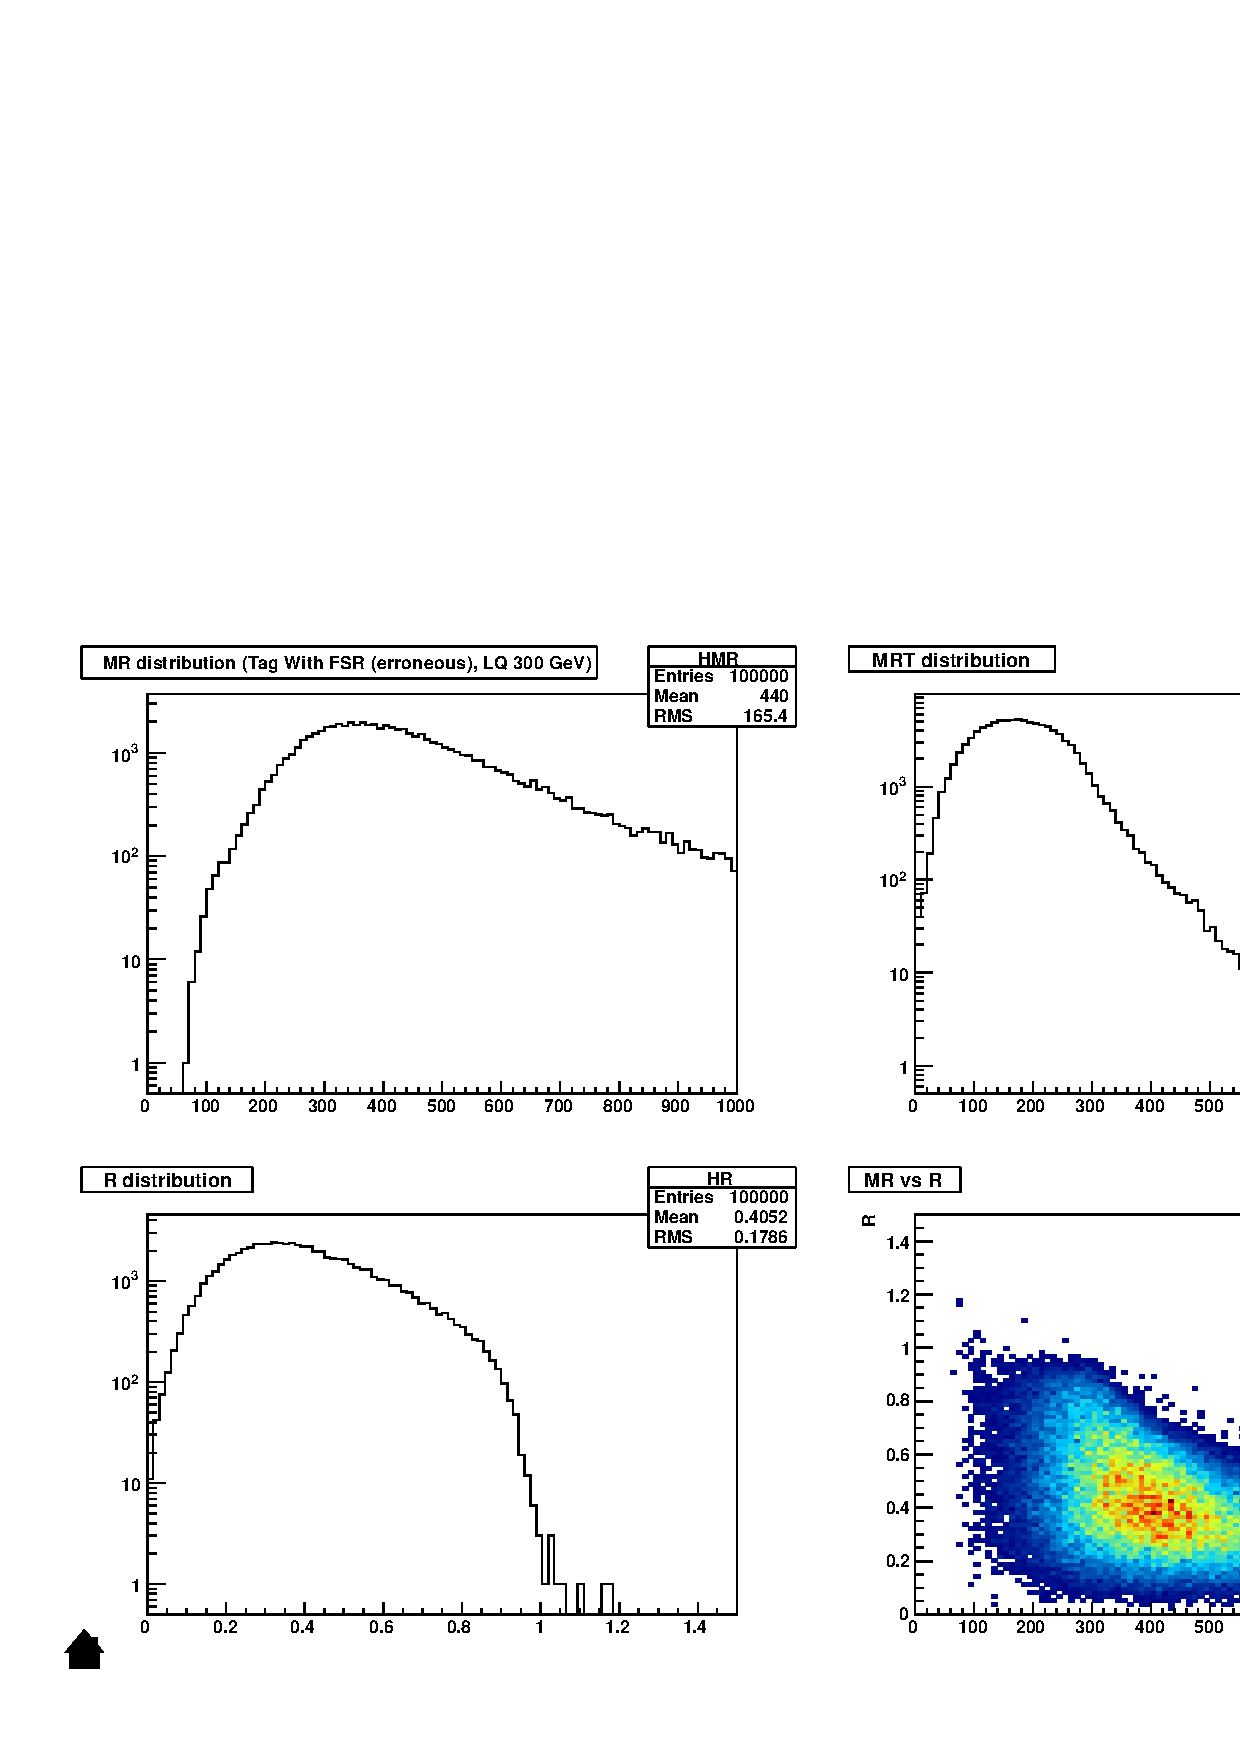
\includegraphics[width=7cm]{Figures/MRToy11_FSR_Hemisphere}
   \caption{Look at pythia8-generated LQ sample before hadronization step, switching on/off different components.  Upper left: hard process only.  Upper right: hard process + multiple interaction.
   Lower left: hard process + ISR.  Lower right: hard process + FSR (errorneous).  Variables constructed by first clustering into jets and then divide into hemispheres.}
   \label{Figure_MRToy11_Hemisphere}
\end{figure}

\begin{figure}[htbp]
   \centering
   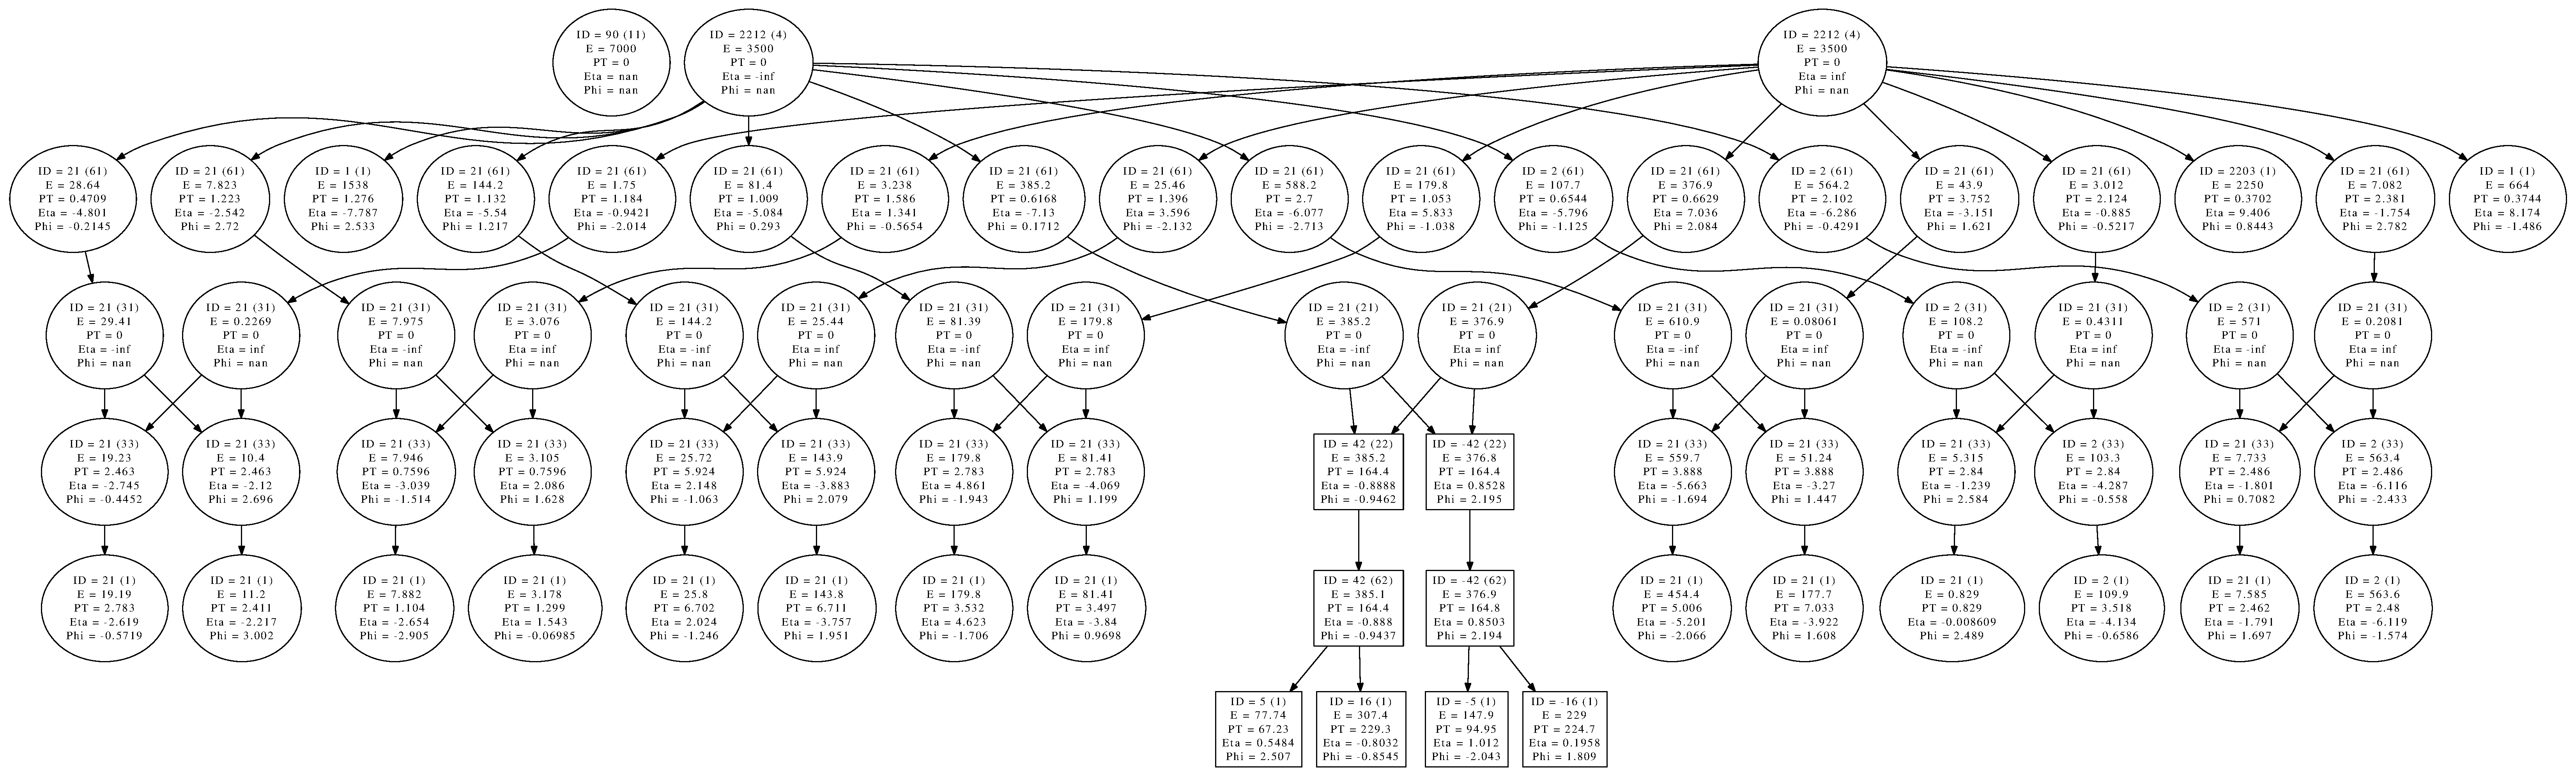
\includegraphics[width=15cm]{Figures/Pythia8MIExample}
   \caption{Example of pythia 8 process with hard process and multiple interactions.  ISR and FSR are turned off in this case.  None of the extra interactions are hard enough in transverse momentum.}
   \label{Figure_Pythia8MIExample}
\end{figure}

\subsection{MRToy 14, different acceptance cut}

In this toy I tried to see if restricting the direction of the two jets (in terms of $\eta$) will make a difference.
The toy progress as usual like the other ones, except that I only accept the ``event'' if both jets are in the acceptance.
See figure \ref{Figure_MRToy14}.   The first four plots show the result while tightening the $\eta$ cut little by little.

Few observations:
\begin{enumerate}
\item Low $M_R$ region disappeared.  This means that with $\eta$ requirement, cut on $M_R$ doesn't really sacrifice us anything.
\item In the main peak, low $R$ region is suppressed.  This is also good news, since a cut on $R$ will also be less harmful to signal.
\item The high $M_R$, low $R$ region is diluted.
\end{enumerate}

The last two plots show the result if we restrict ourselves to a strange band in $\eta$.
Indeed, it is in accordance with observations above: higher $\eta$ range maps preferrably to low $M_R$ or low $R$ region.
This also means that by moving towards upper-right corner in the $R-M_R$ plane, the jets are more central.

\begin{figure}[htbp]
   \centering
   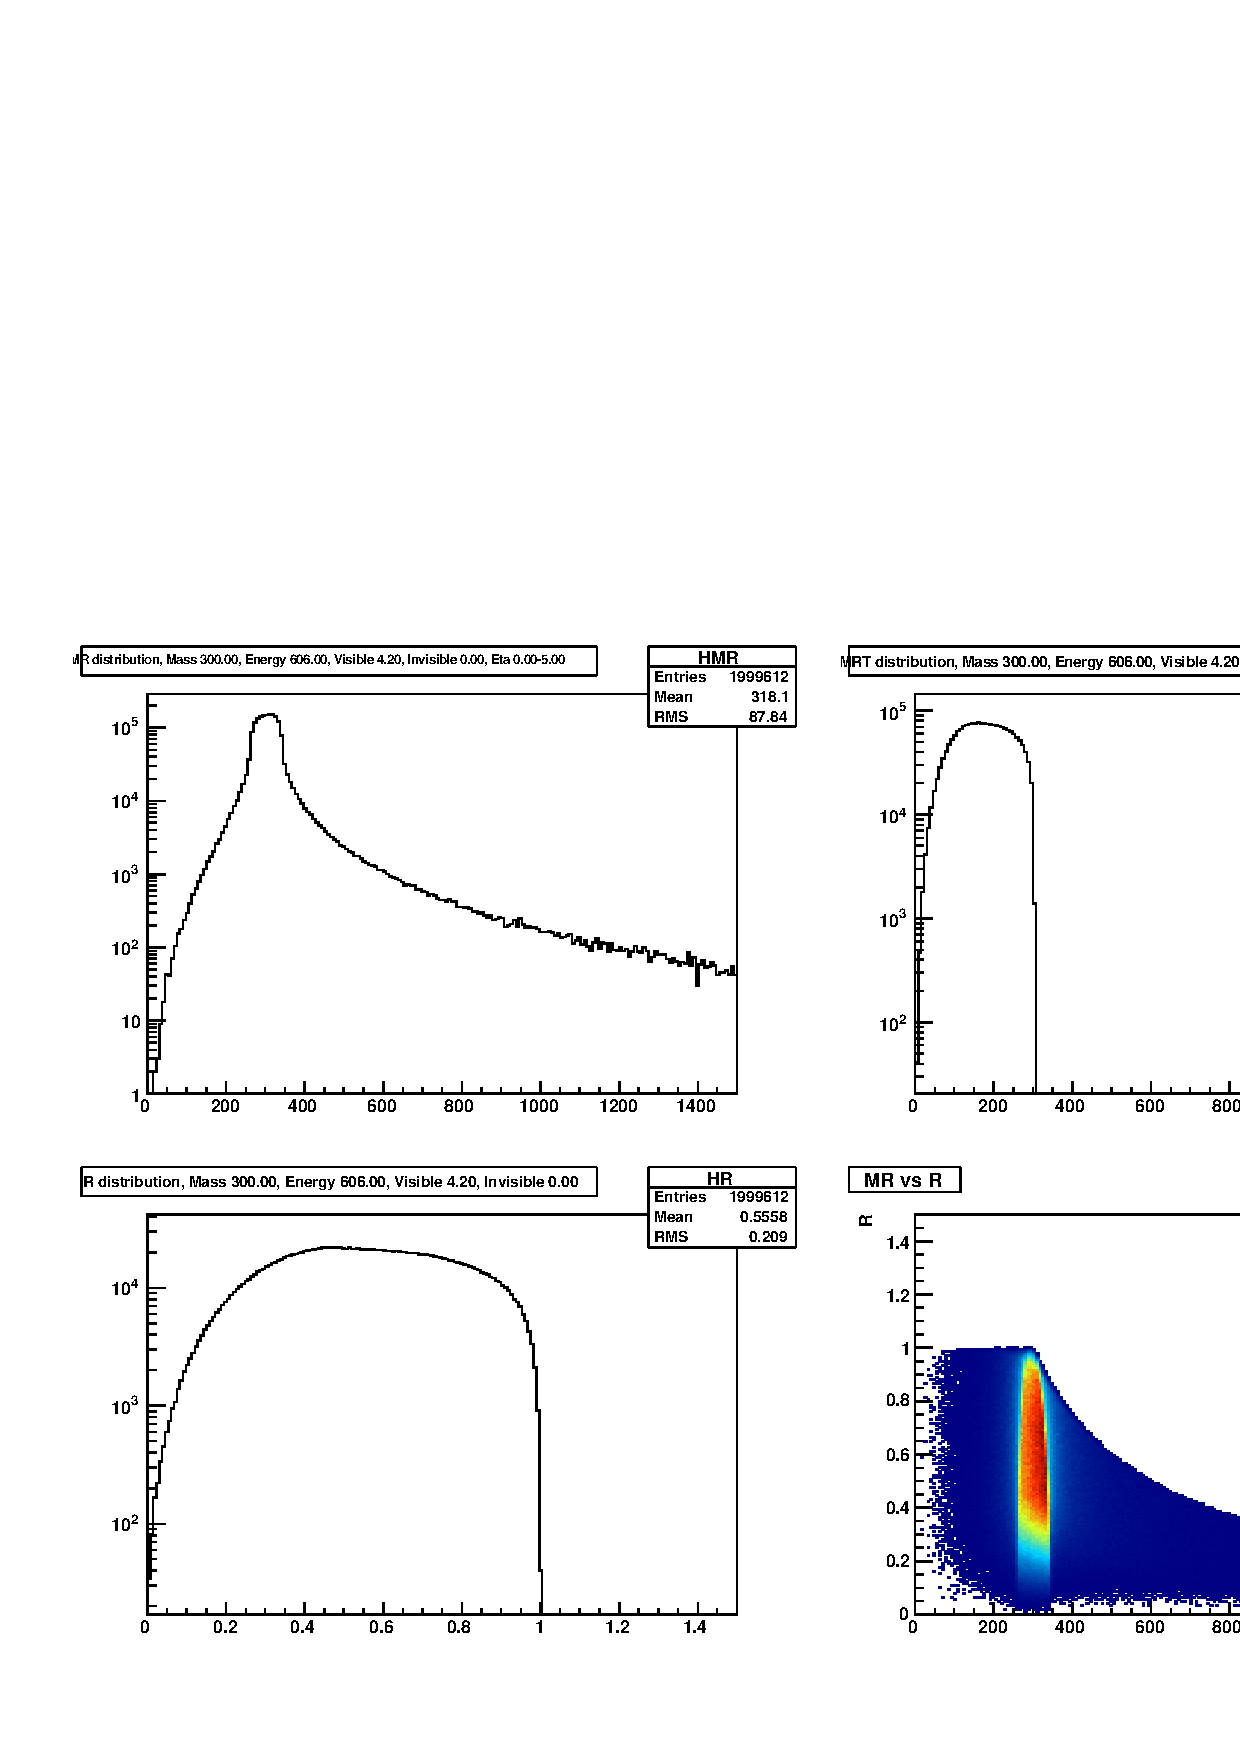
\includegraphics[width=7cm]{Figures/MRToy14_NoCut}
   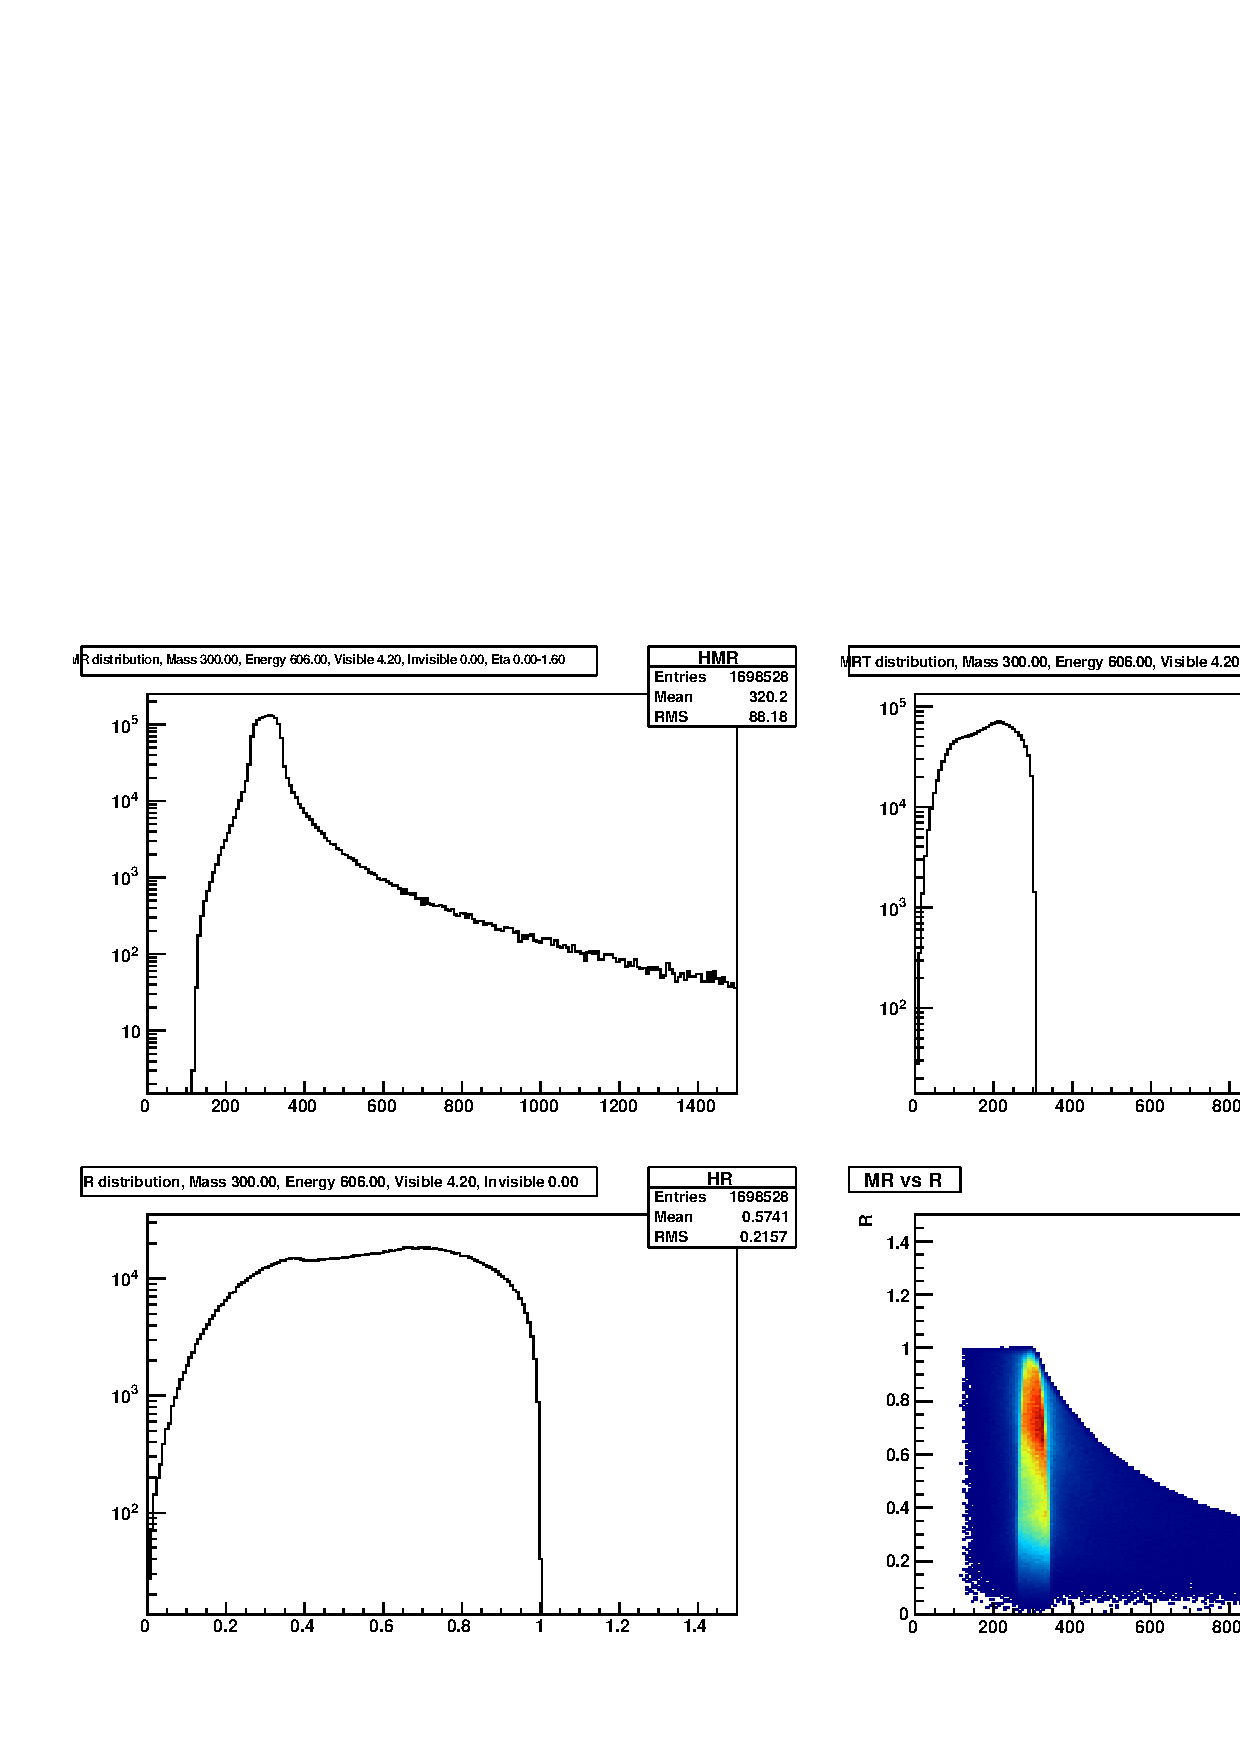
\includegraphics[width=7cm]{Figures/MRToy14_ToEndcap}\\
   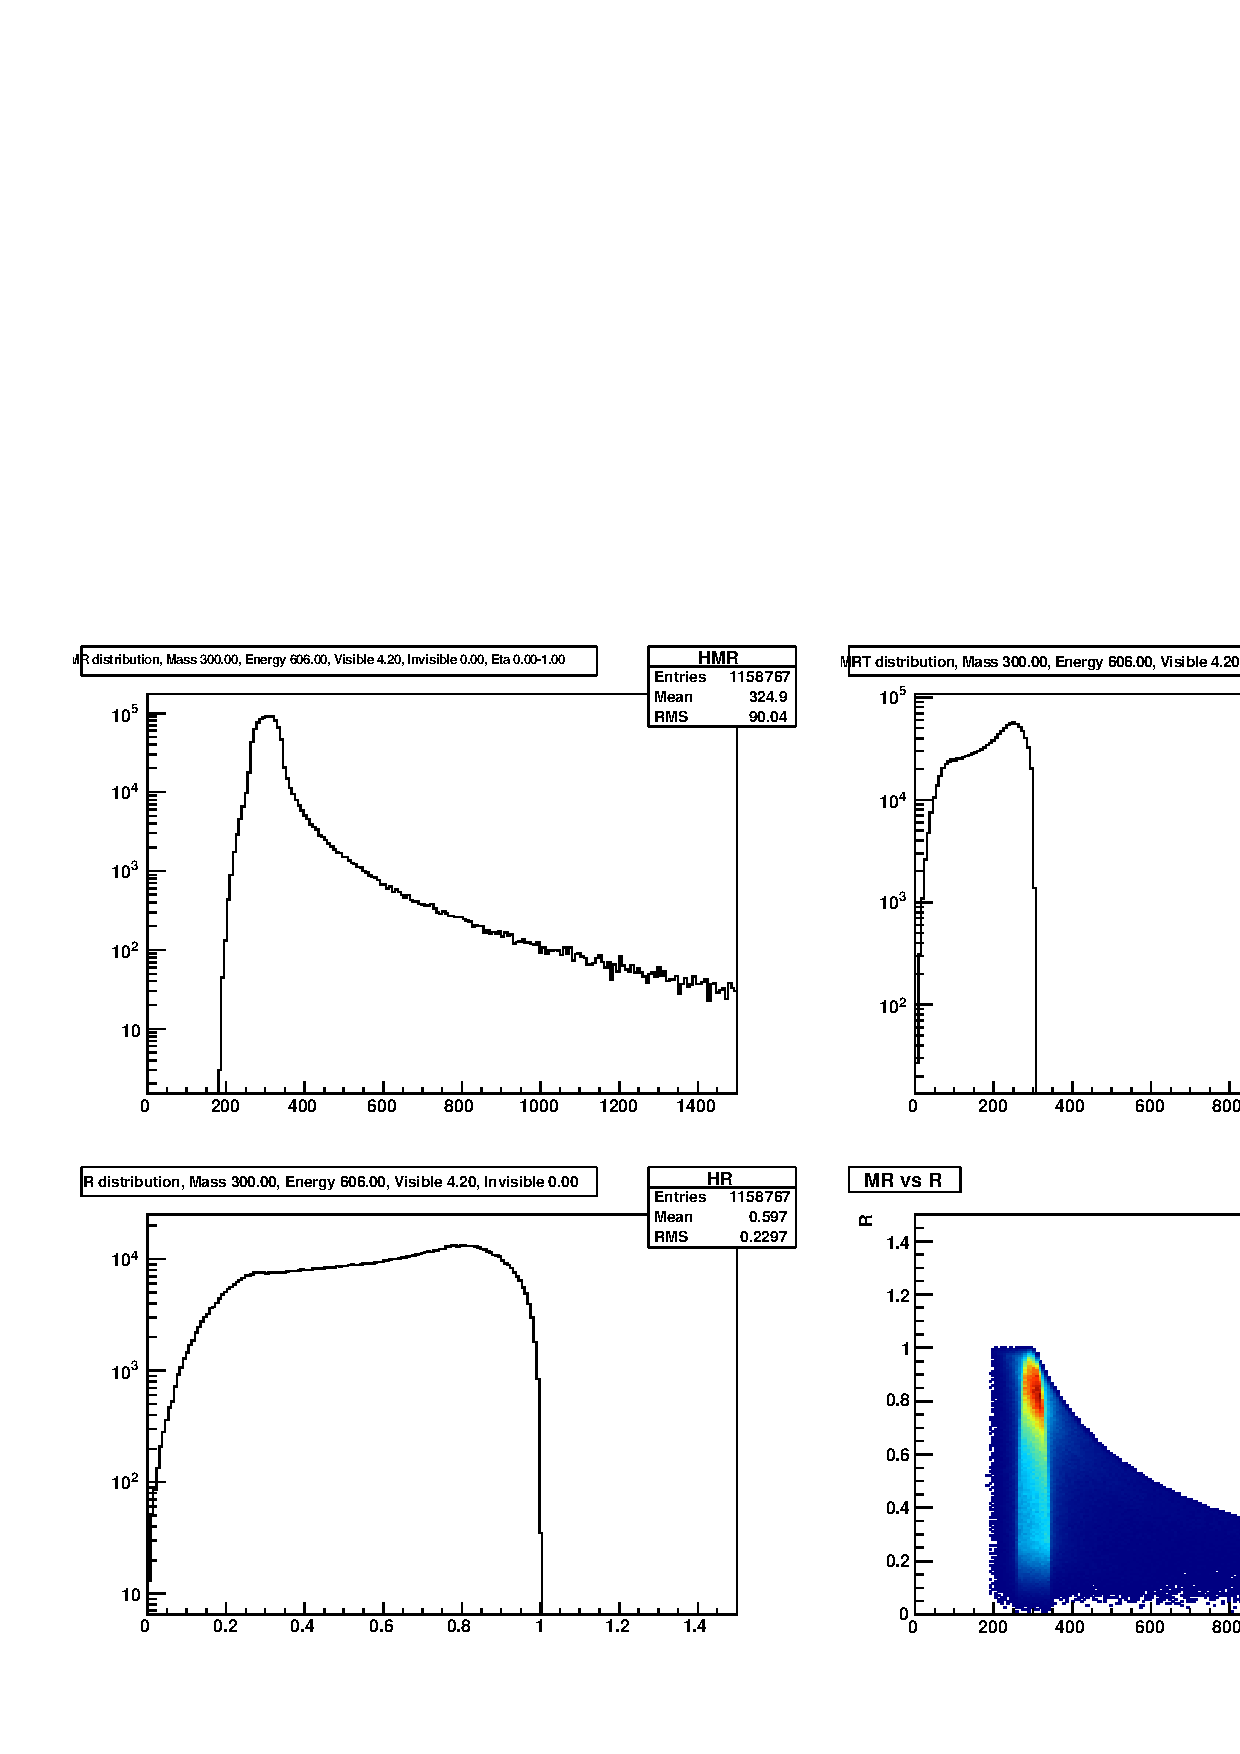
\includegraphics[width=7cm]{Figures/MRToy14_ToBarrel}
   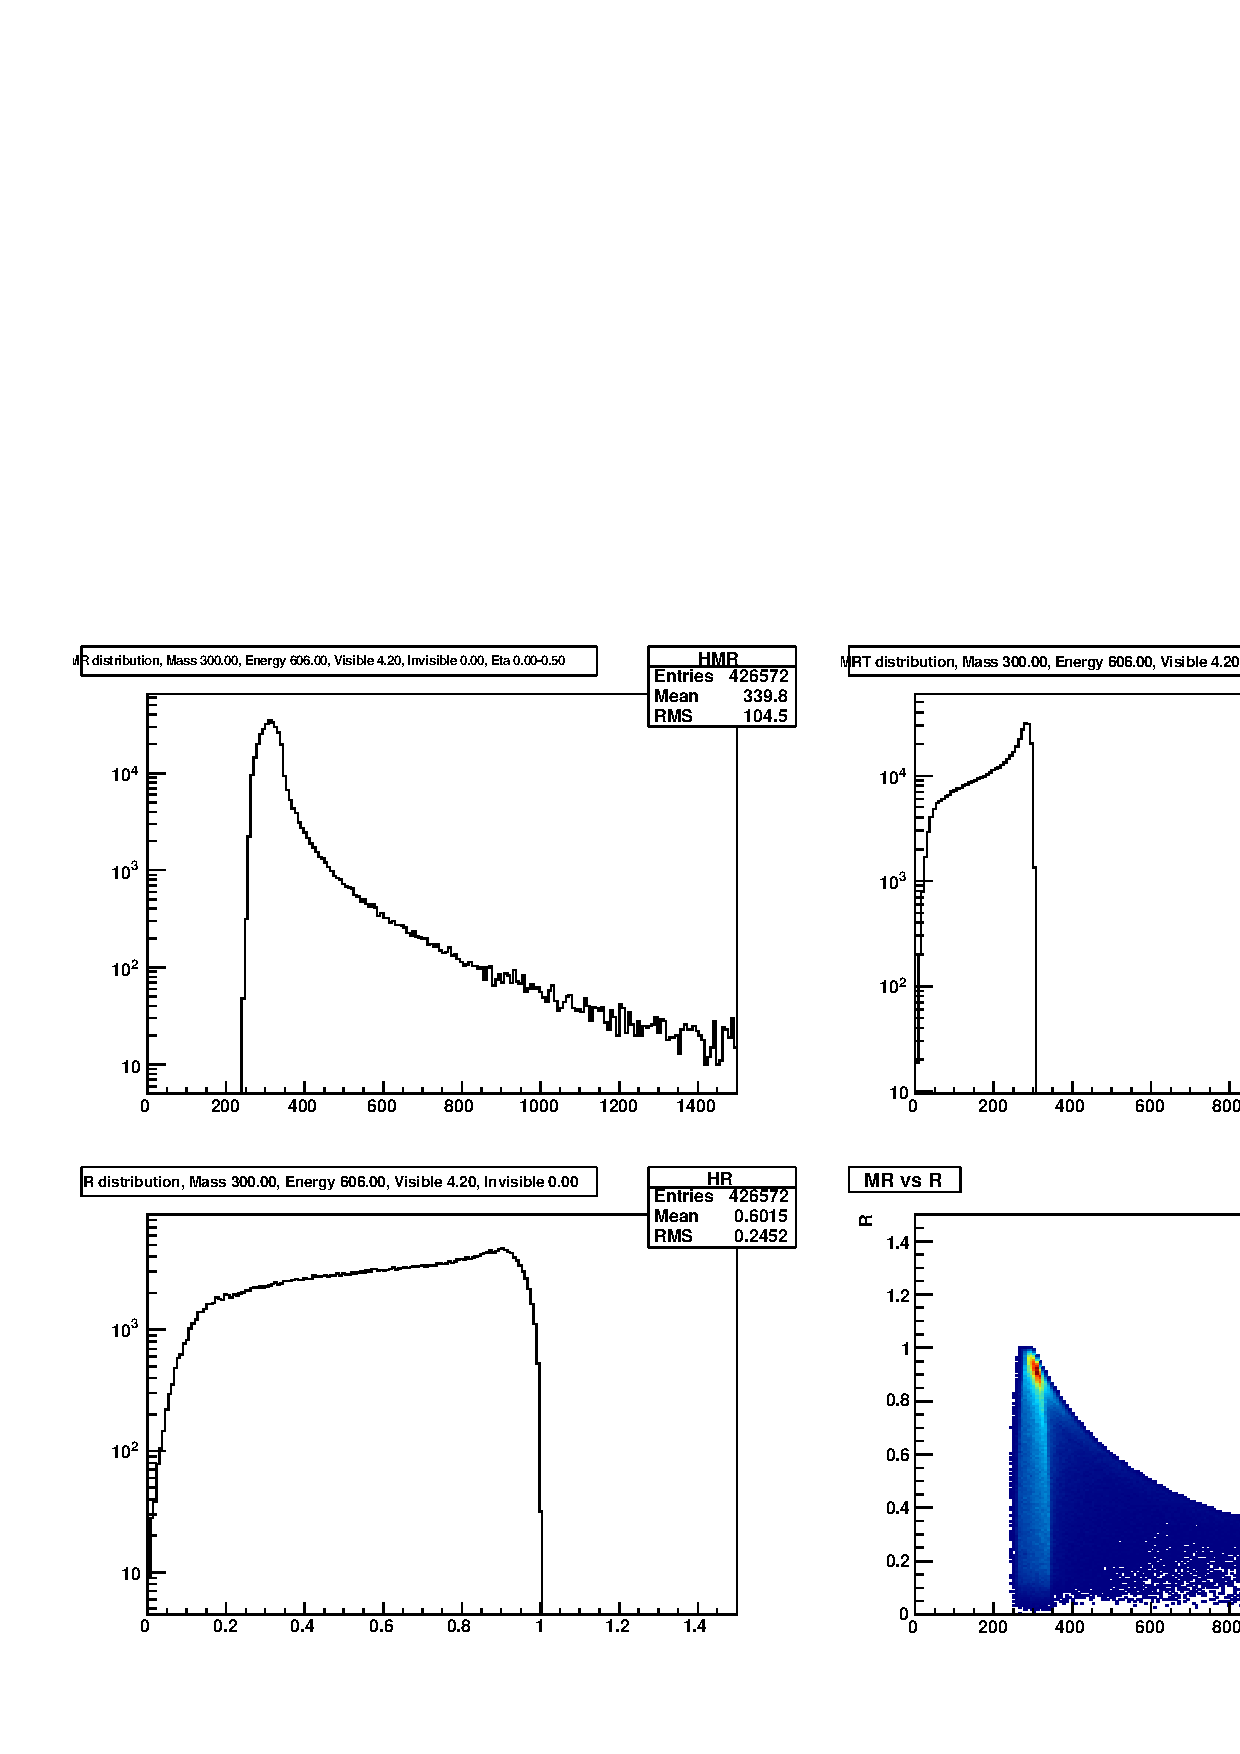
\includegraphics[width=7cm]{Figures/MRToy14_Central}\\
   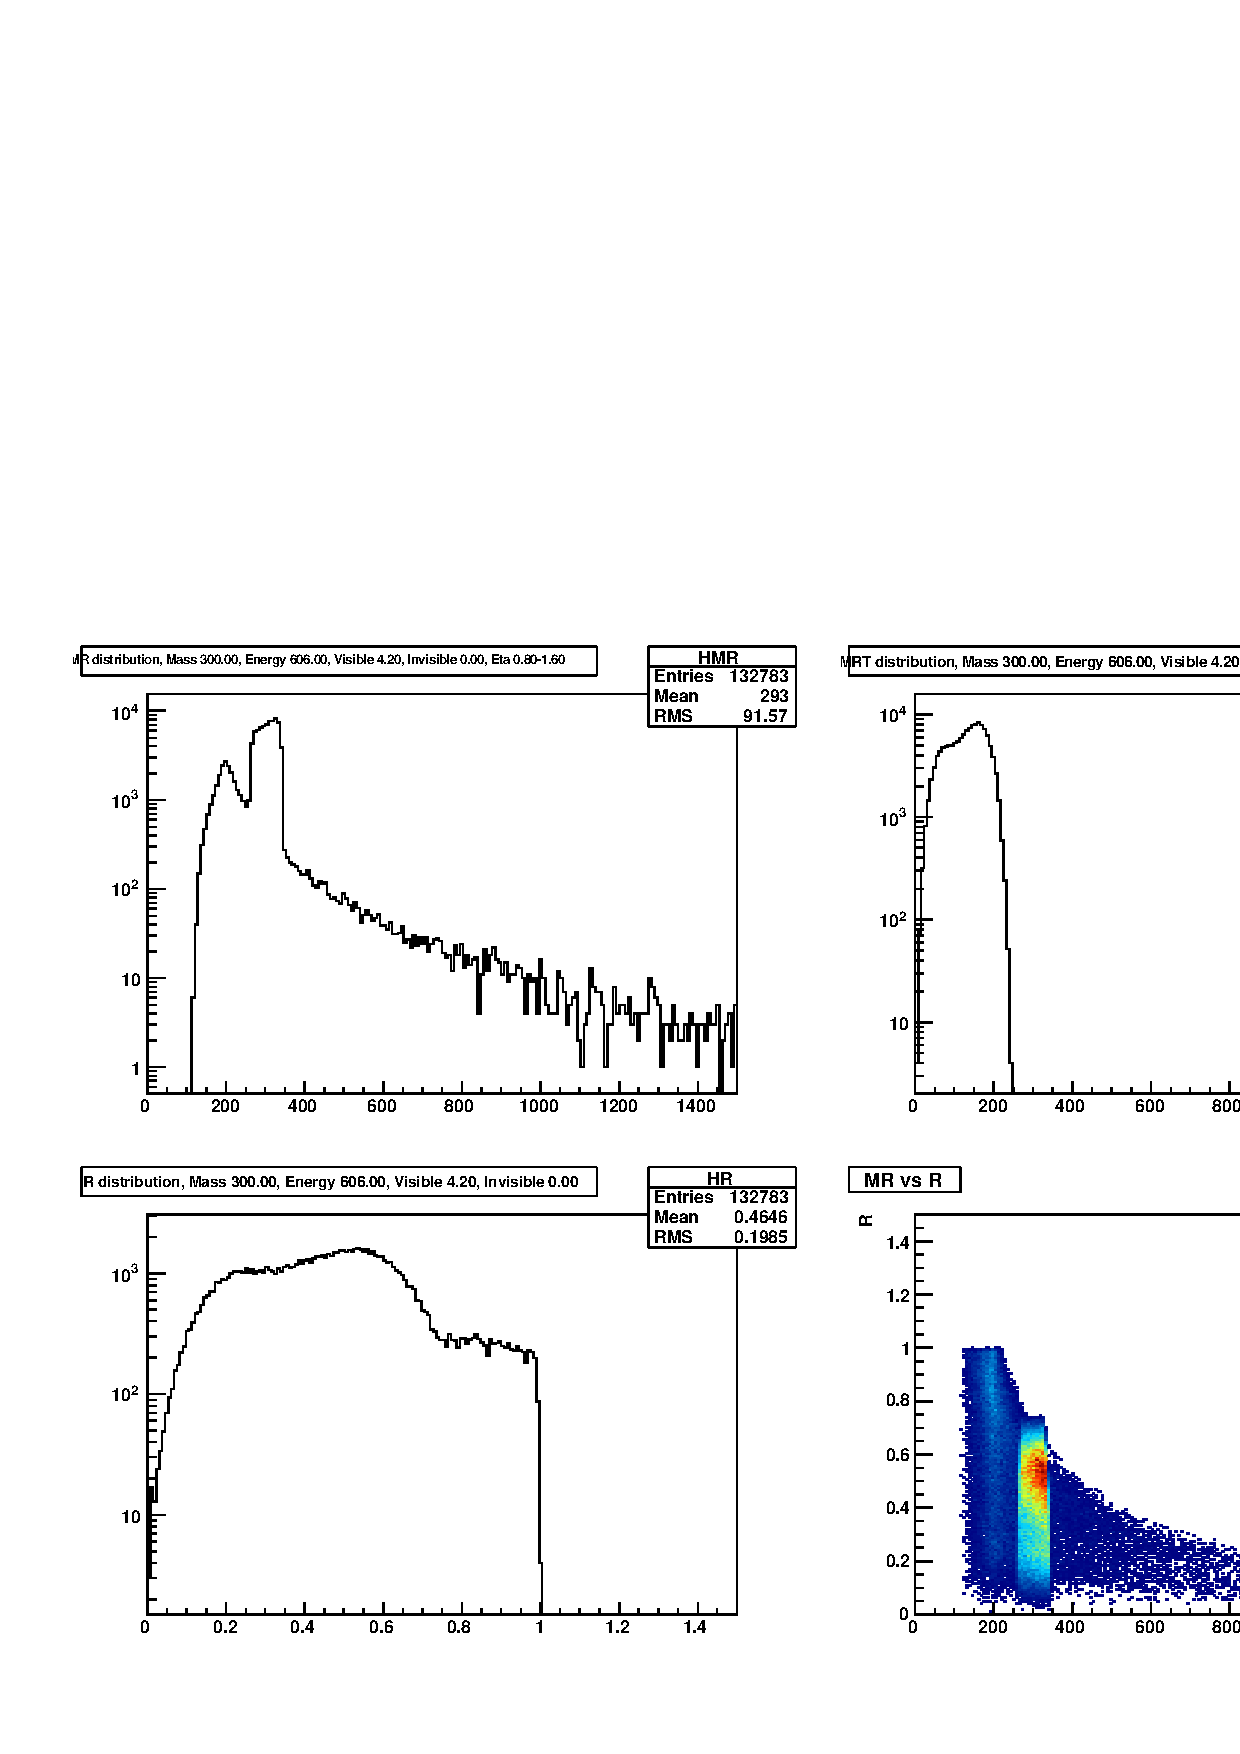
\includegraphics[width=7cm]{Figures/MRToy14_HalfBarrel}
   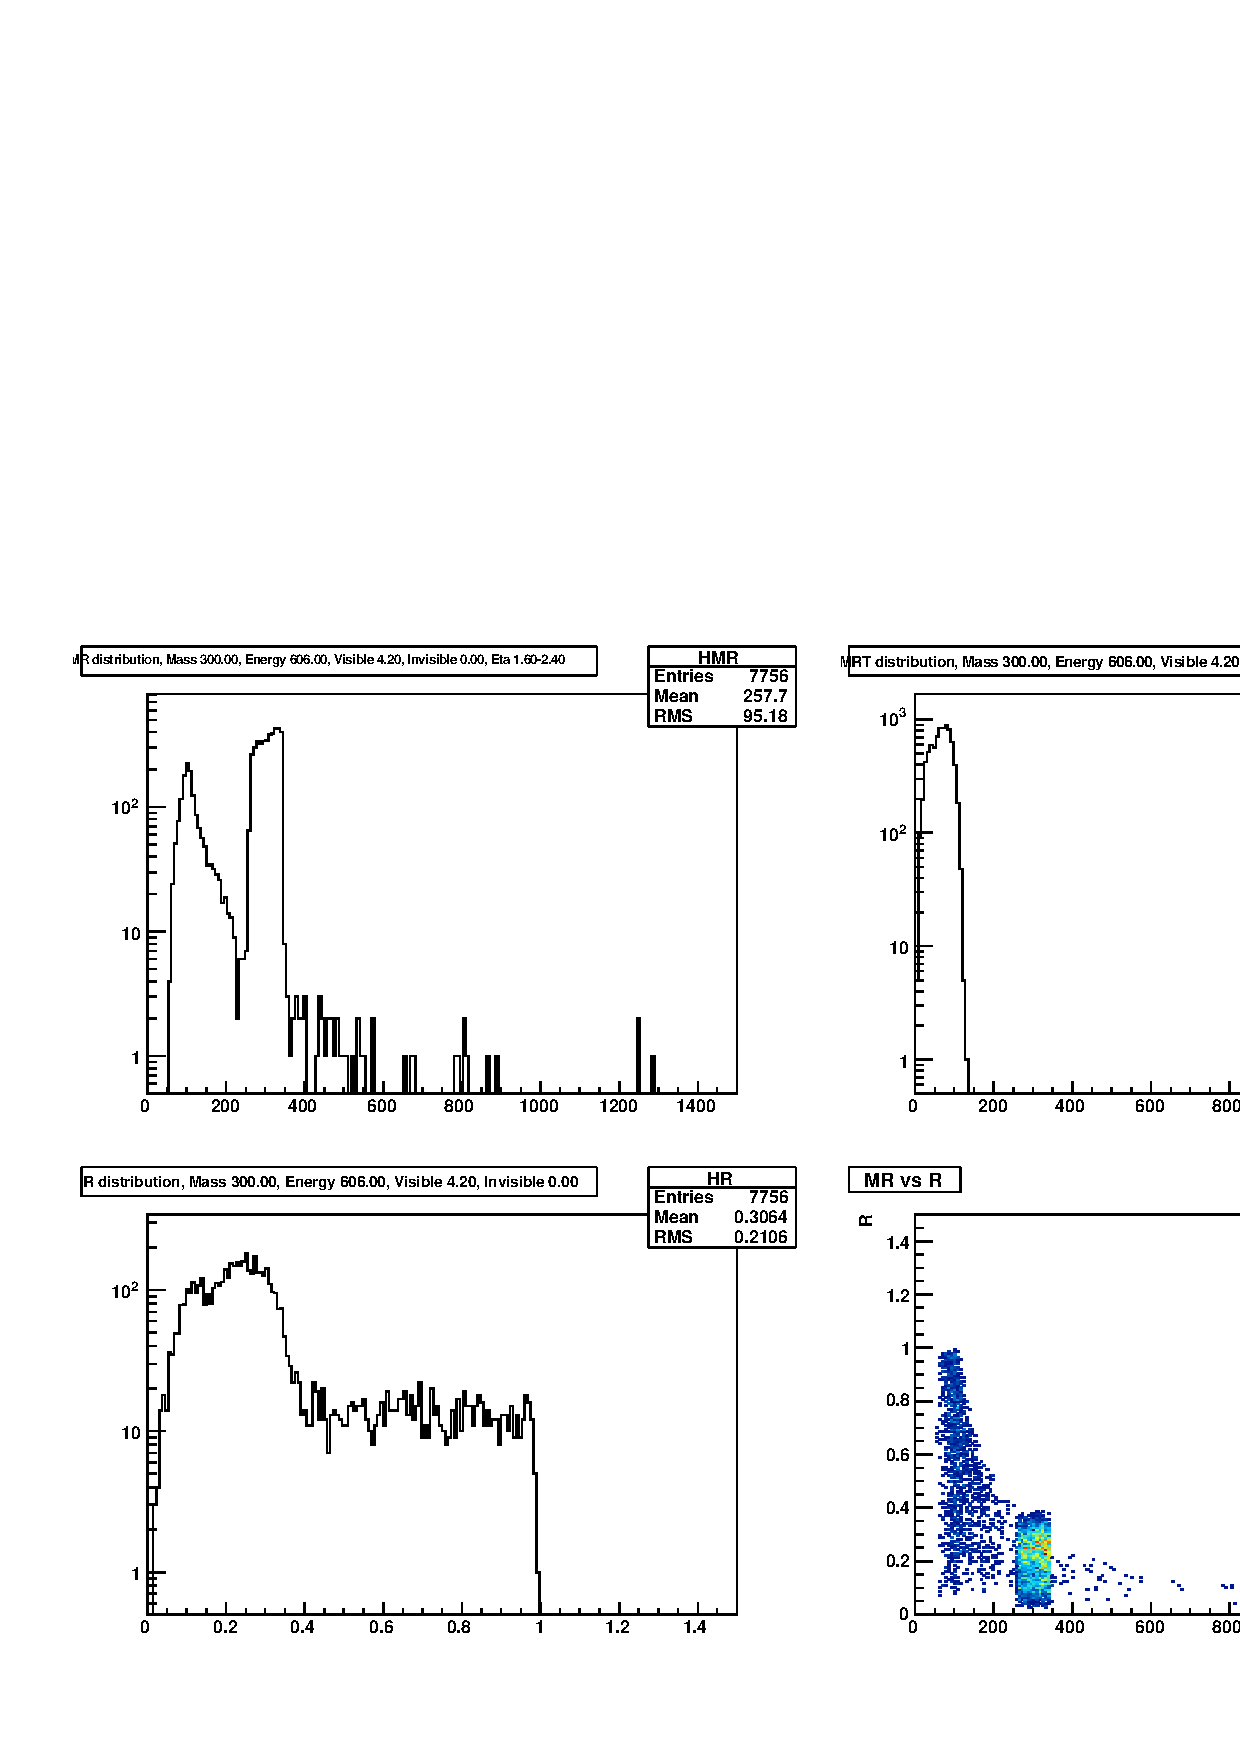
\includegraphics[width=7cm]{Figures/MRToy14_Endcap}
   \caption{Changing $\eta$ cut while calculating the magic variables.  Upper left: no cut, upper right: $\eta$ up to 1.6, central left: $\eta$ up to 1.0,
   central right: $\eta$ up to 0.5, lower left: $\eta$ from 0.8 to 1.6, lower right: $\eta$ from 1.6 to 2.4}
   \label{Figure_MRToy14}
\end{figure}

\subsection{MRToy15.  Effect of holes in detector}

In reality it is very likely that some part of detector may fail (single channel, group of channels, etc.).
So let's run toys to see what the effect is.
It is hard to see the deficit when acceptance has holes since the change is small, so what is plotted here, instead, is the distribution
when one of the two final visible particles/jets/megajets fall into the hole.
The total number of tries is 10M in each case here, so in addition we can roughly see the efficiency drop (to the order of magnitude at most)
due to holes.  In reality it will be better since jets won't disappear just because of a tiny hole.  In this case please refer to other toys (Toy number 3)
with scale smearing to see the effect.
As seen in figure \ref{Figure_MRToy15}, it's consistent with what was seen in the previous toy where we change $|\eta|$ acceptance cut.
With this failure percentage, we won't be able to see the bias introduced by the strange shape.

\begin{figure}[htbp]
   \centering
   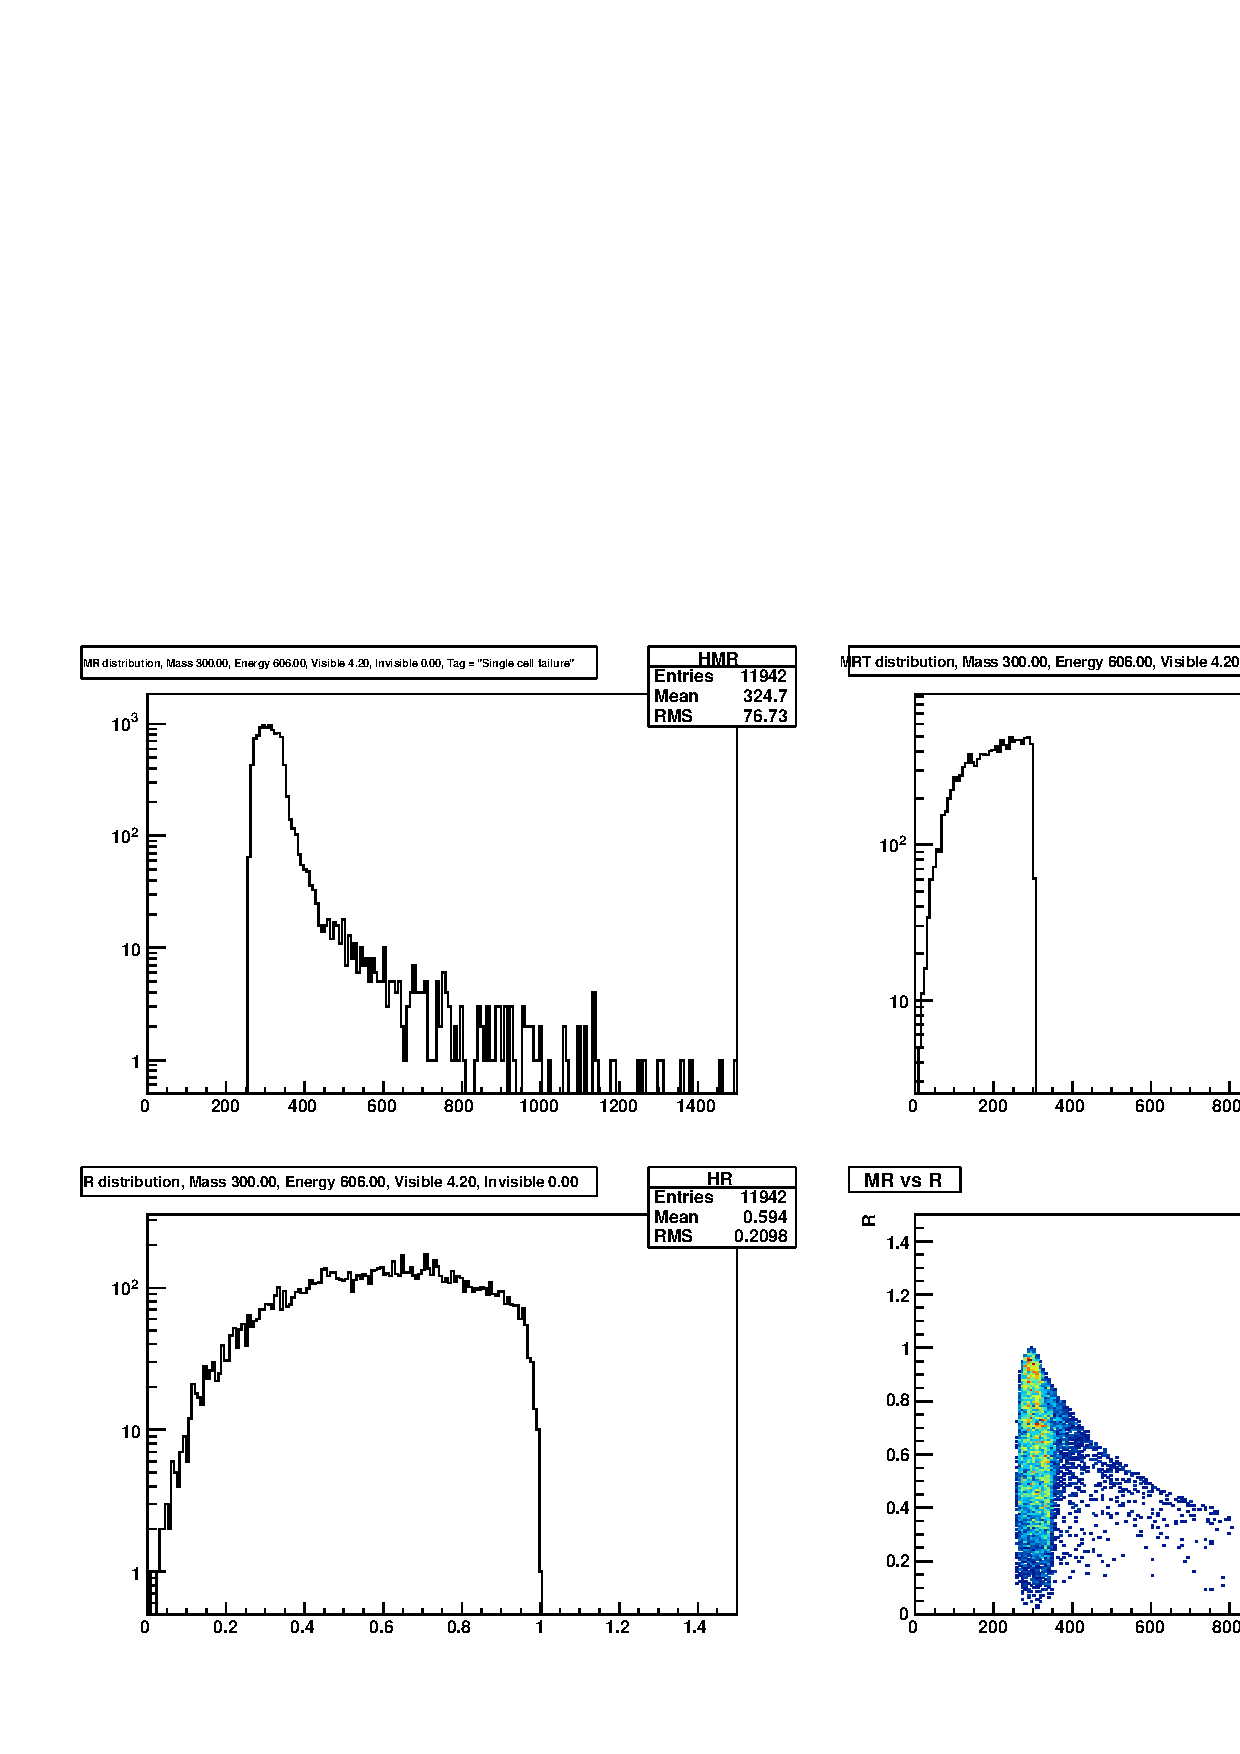
\includegraphics[width=7cm]{Figures/MRToy15_SingleChannel}
   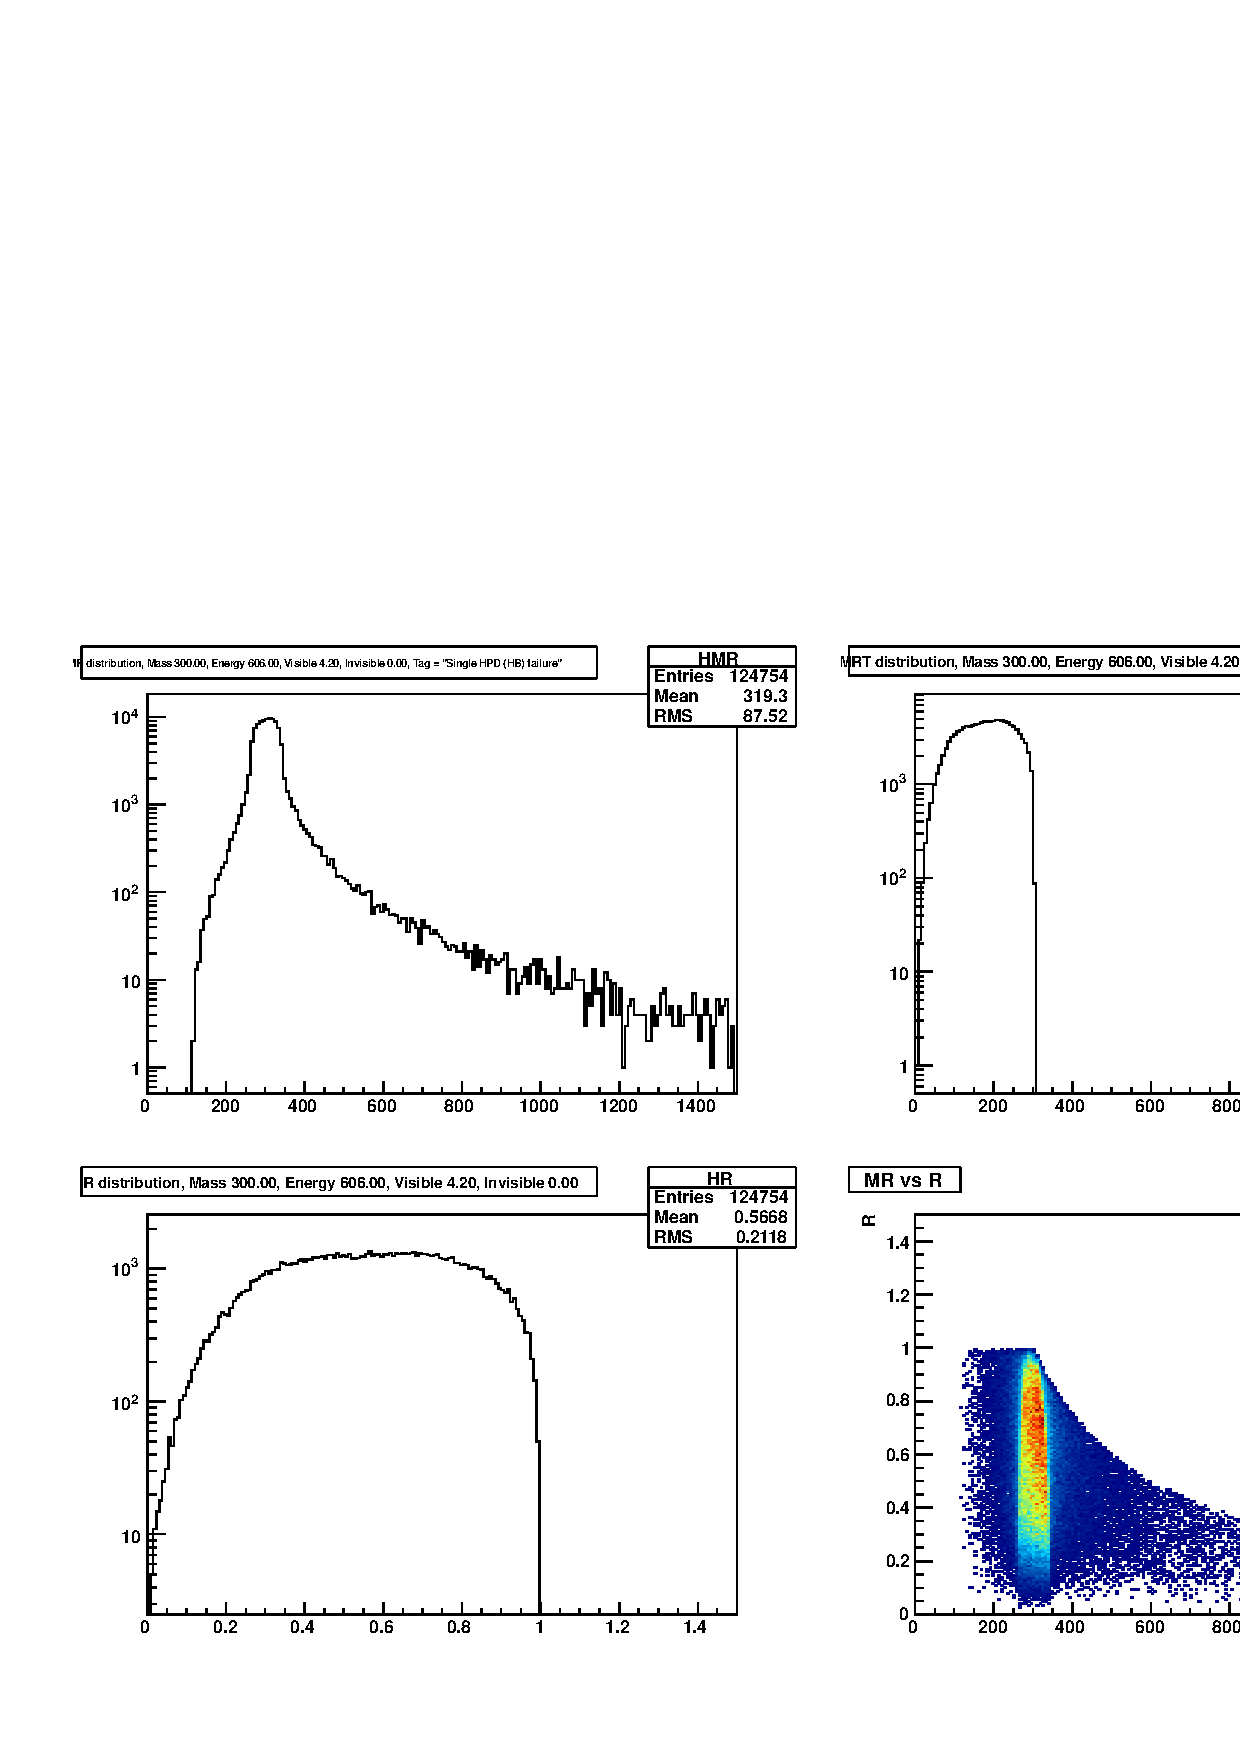
\includegraphics[width=7cm]{Figures/MRToy15_HBHPD}\\
   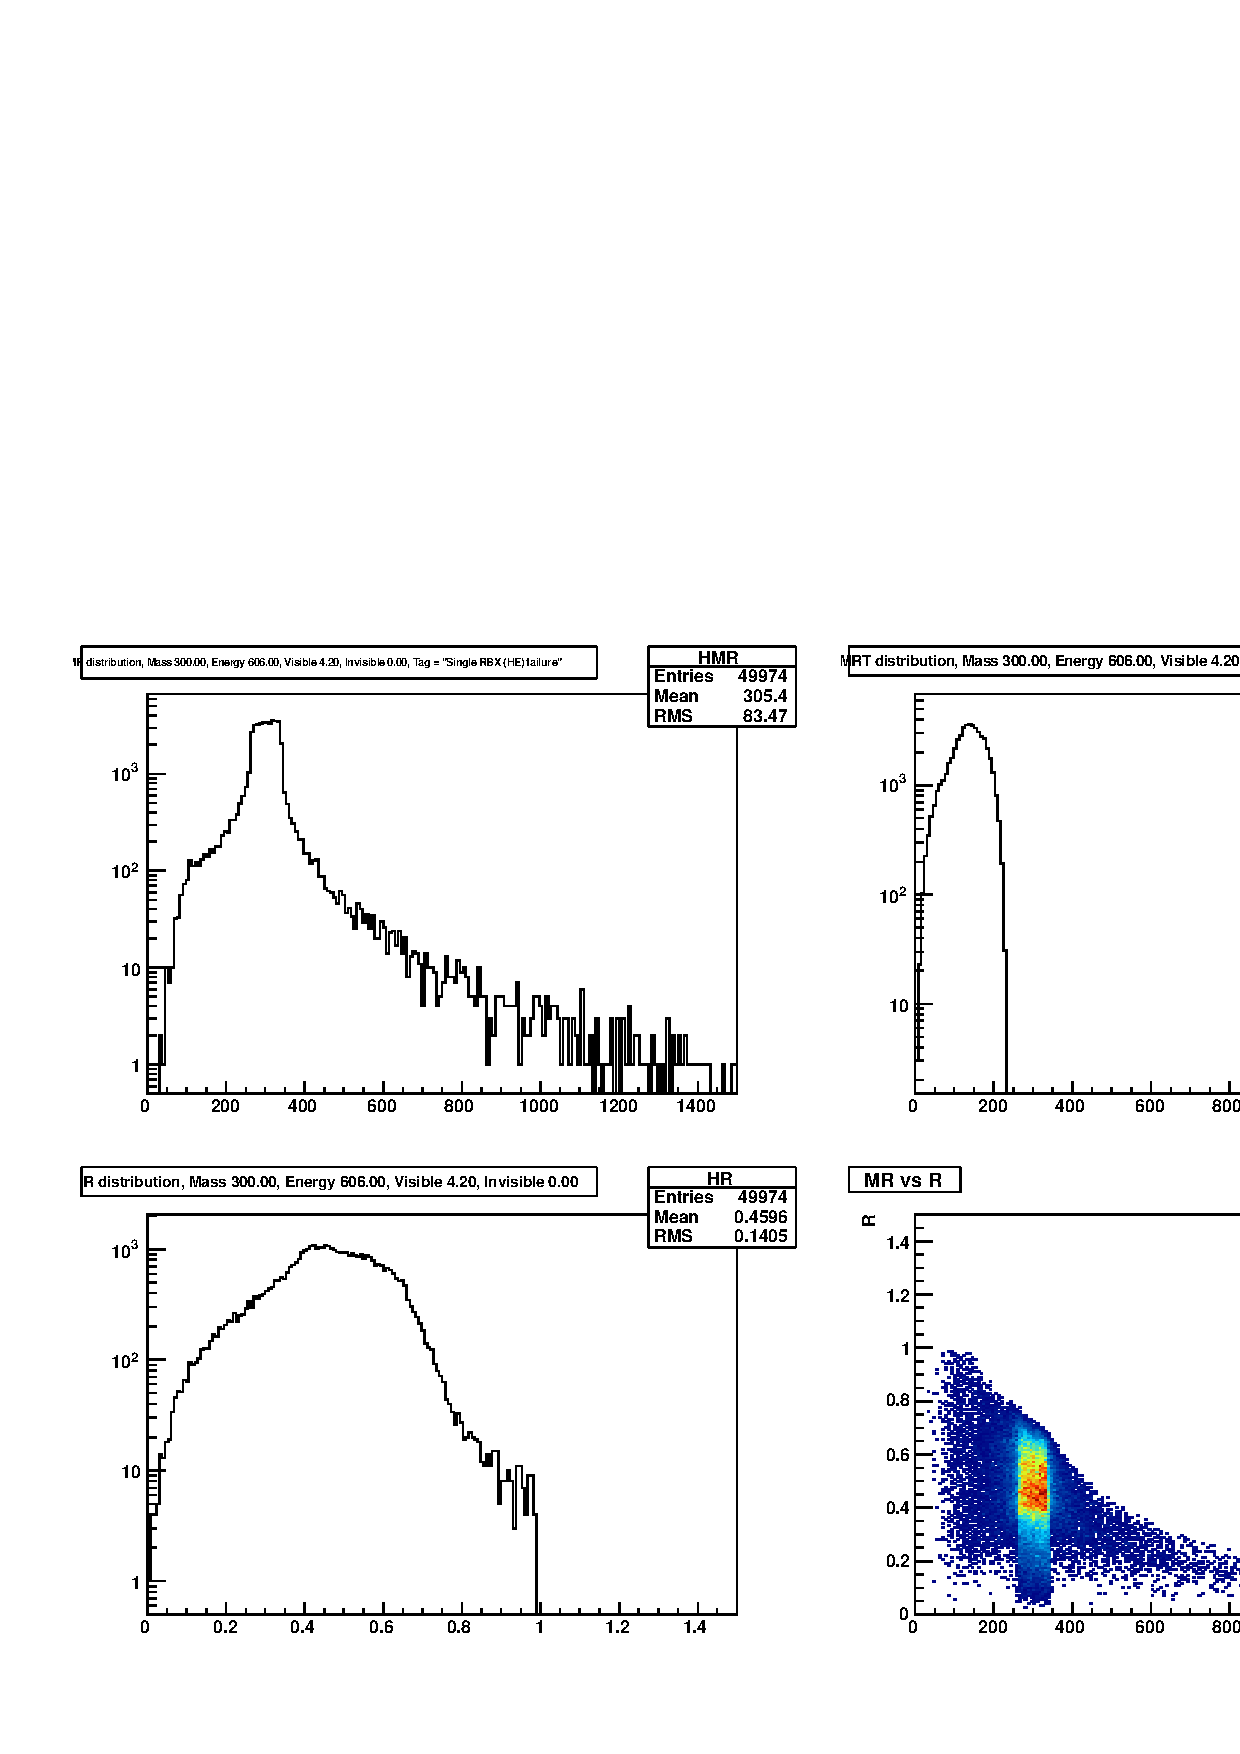
\includegraphics[width=7cm]{Figures/MRToy15_HERBX}
   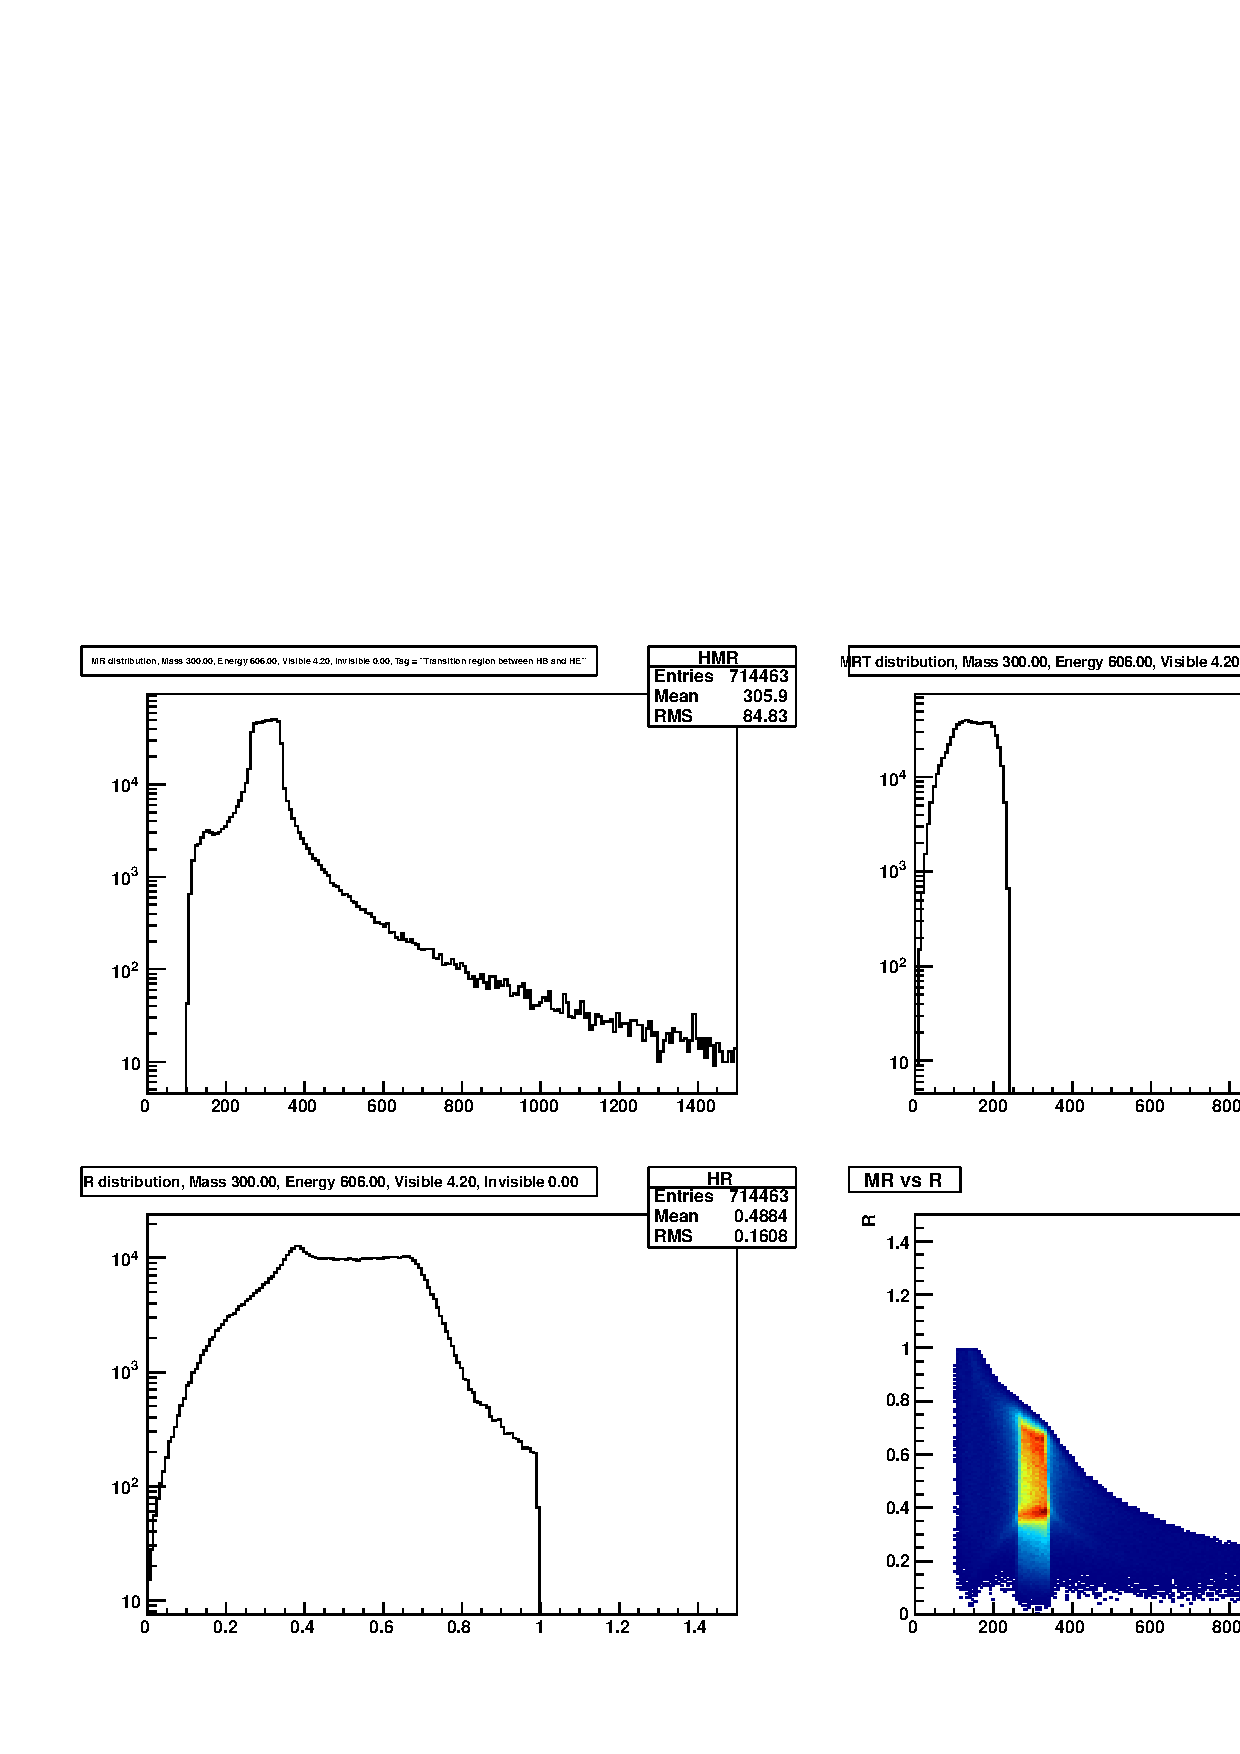
\includegraphics[width=7cm]{Figures/MRToy15_Transition}
   \caption{Holes in the detector.  Upper left: central, single channel failure (0.087x0.087 in $\eta-\phi$ space).  Upper right: Single HPD failure, central again.
   Lower left: single HE RBX failure, lower right: transition region failure ($|\eta| = 1.4-1.6$).  Failure percentage: 0.12\%, 1.2\%, 0.50\%, 7.1\%.}
   \label{Figure_MRToy15}
\end{figure}


\section{Walking through other results in the different toys}

I'll be brief in this section, since the highlights are picked out above.

\subsection{MRToy 1, heavy object boost in the hard-process-CM frame}

$R$ doesn't change much since it's a geometrical cut, not absolute scale.
In $M_R$ the plateau becomes larger, mostly because of the phase space opened up by the boost of heavy object which makes light object decay angles matter.
When there is no boost, the angle doesn't matter.  Shown in figure \ref{Figure_MRToy1}.

\begin{figure}[htbp]
   \centering
   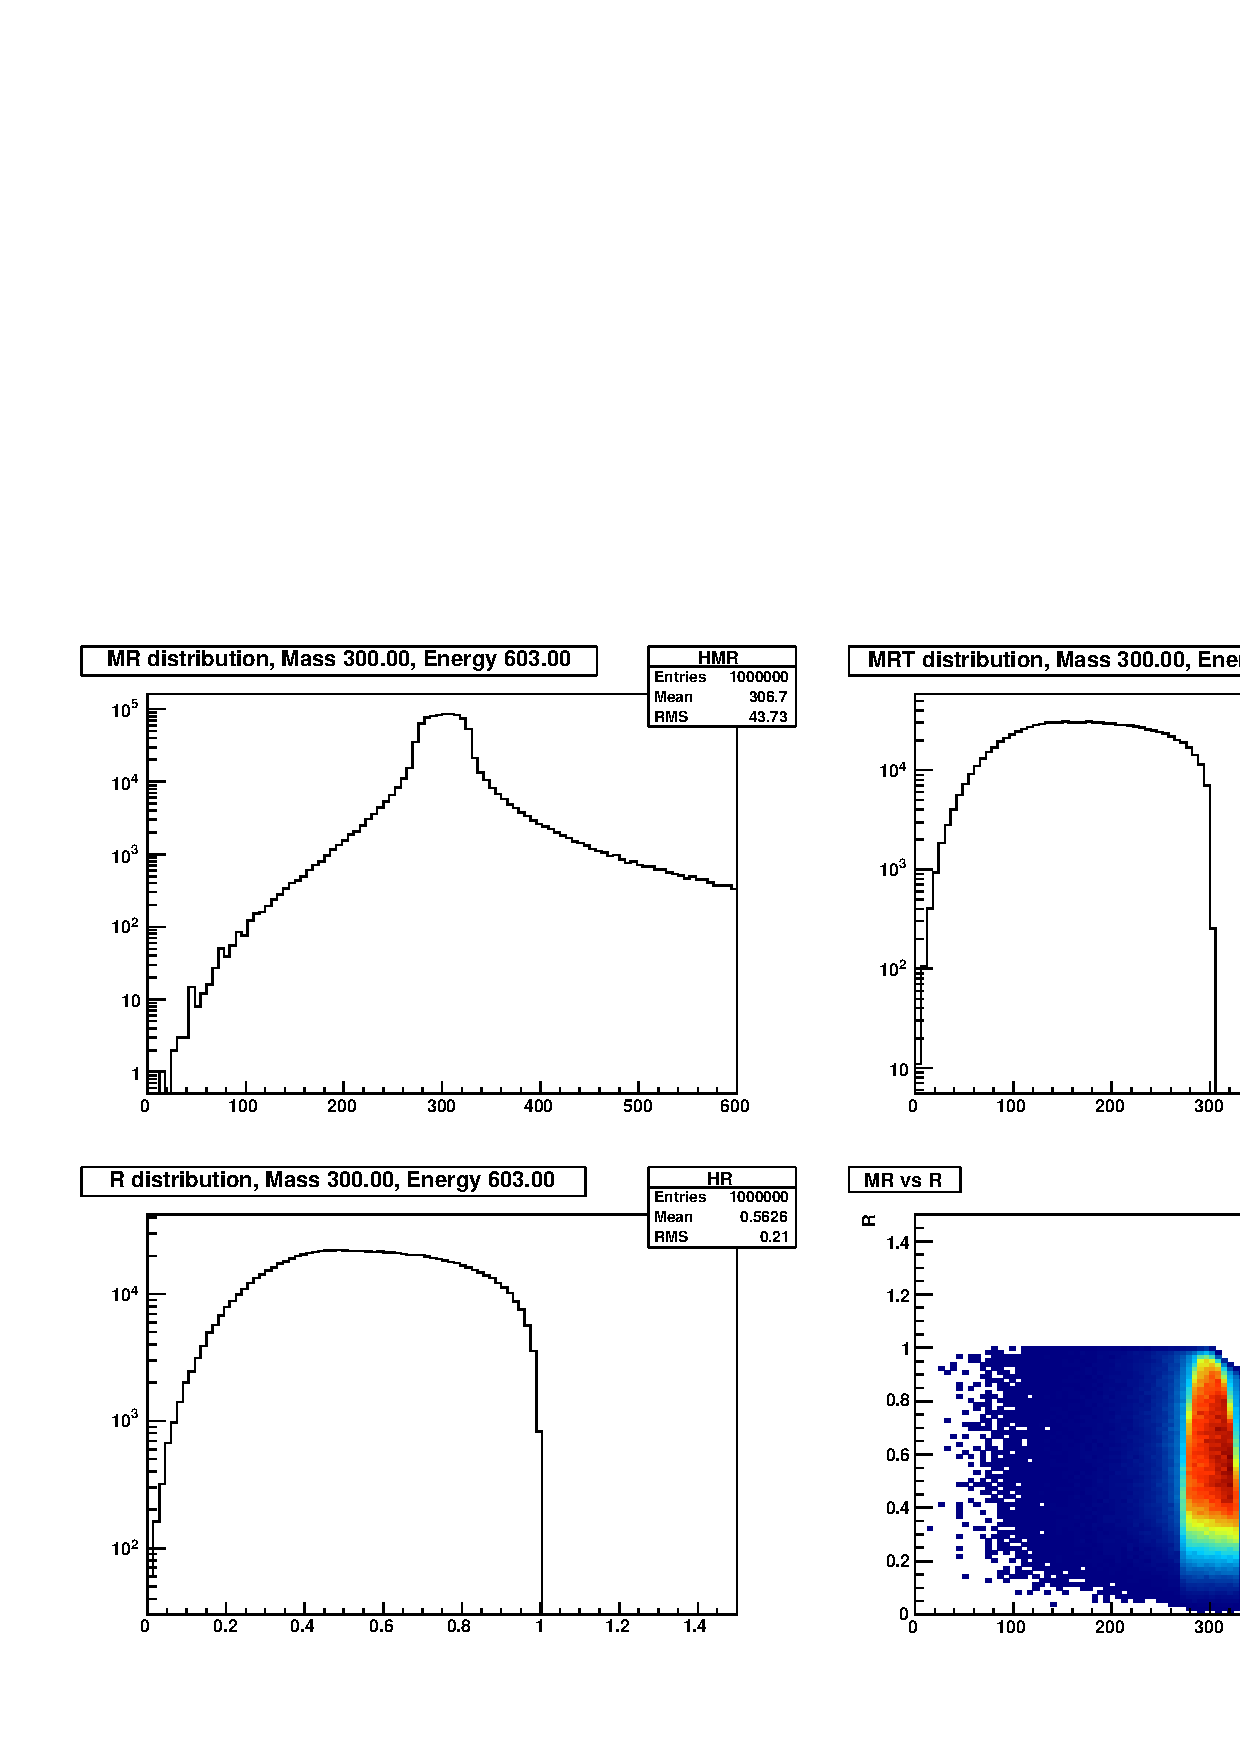
\includegraphics[width=7cm]{Figures/MRToy1_SmallGammaCM}
   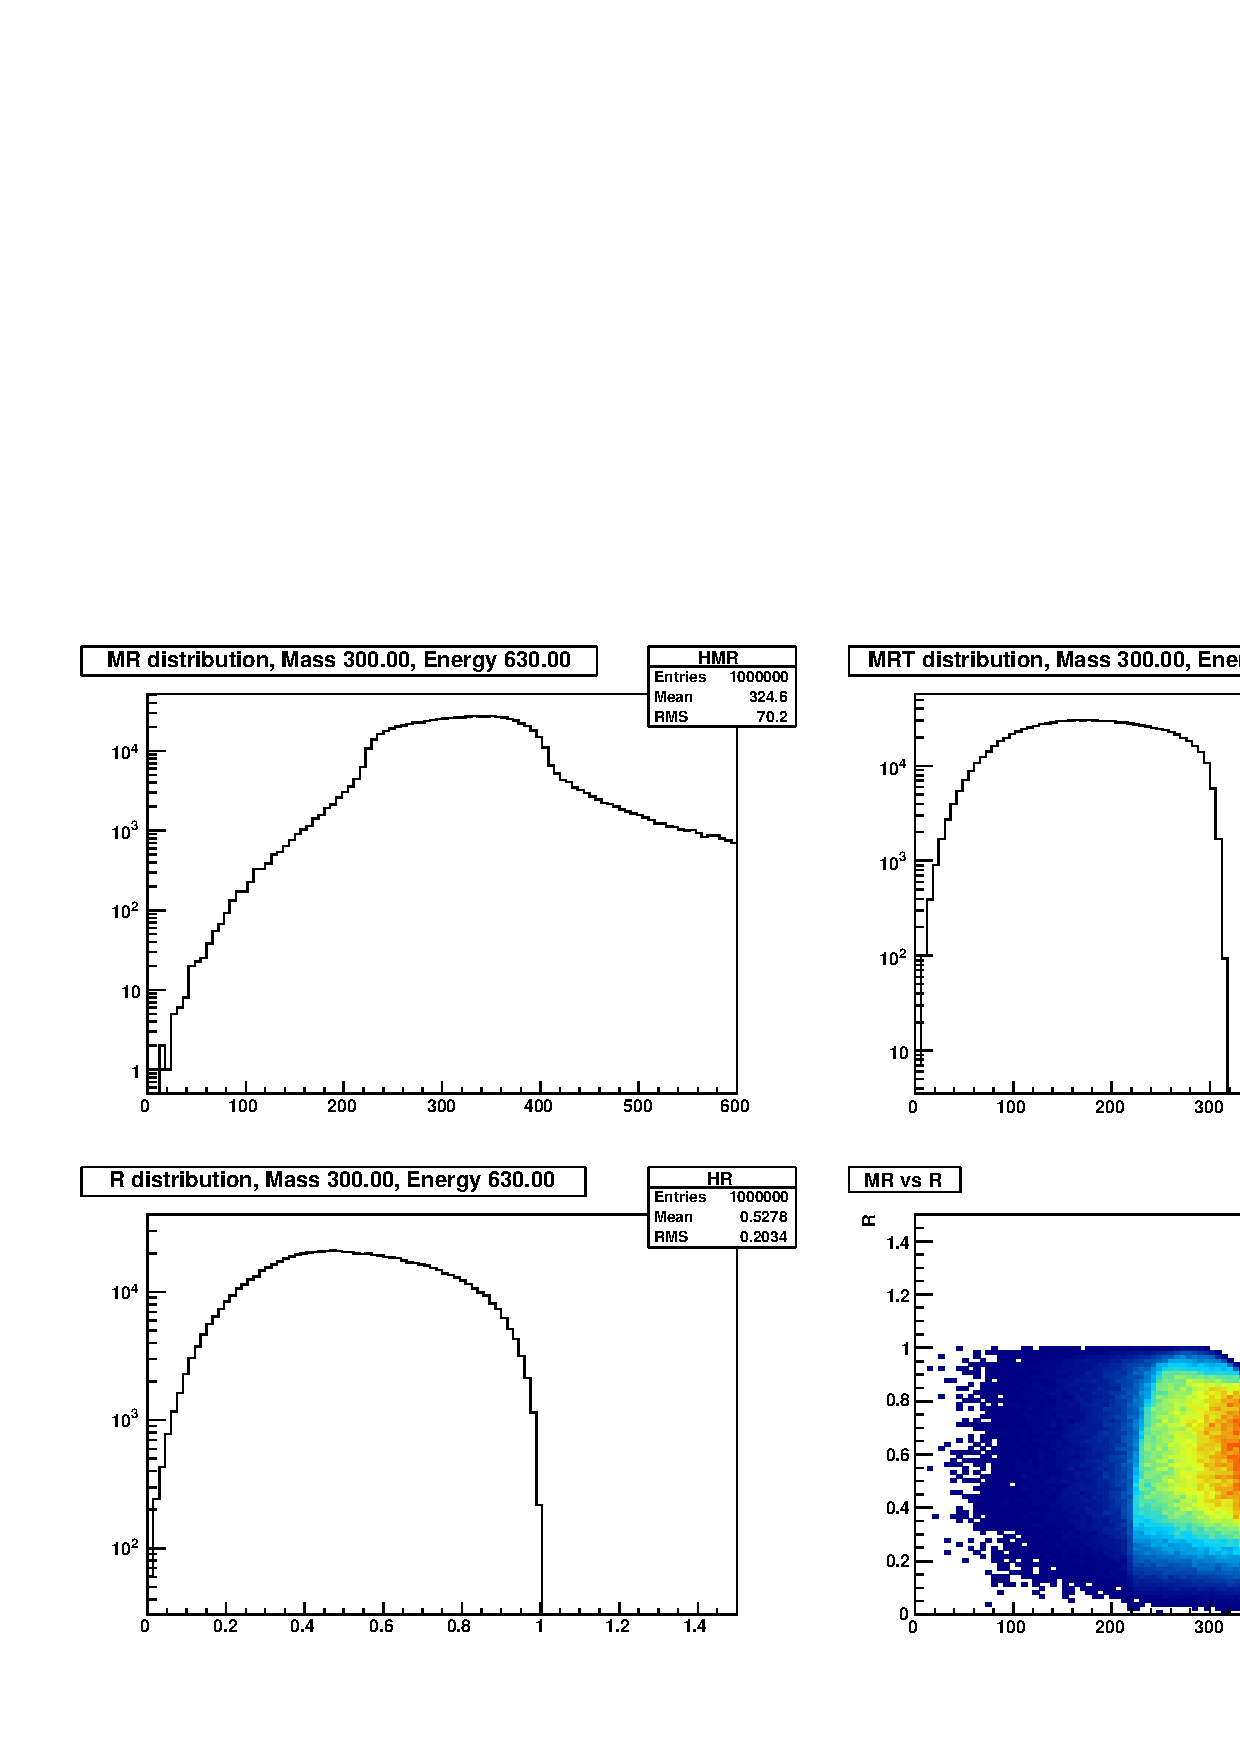
\includegraphics[width=7cm]{Figures/MRToy1_LargerGammaCM}
   \caption{Changing $\gamma_{CM}$, the boost of heavy object in the hard-process-CM frame.  Left: small boost ($\gamma_{CM}$ = 1.005), right: large boost ($\gamma_{CM}$ = 1.05)}
   \label{Figure_MRToy1}
\end{figure}

\subsection{MRToy 3, smearing momentum and angle of various objects}

Here I test the effect on $M_R$ and $R$ via smearing either momentum or angle of visible or invisible objects.
Note that smearing angle of visible is equivalent of smearing invisible particles, so only one is included here for brevity.
Plots are in figure \ref{Figure_MRToy3}.  Here I list the observations.
\begin{enumerate}
\item Scale of visible particle.  Both $M_R$ and $R$ spread out.  Nothing too interesting....
\item Scale of invisible particle.  Of course $M_R$ doesn't change.  Tails start to form in $R$ and $M^{T}_R$.
\item Angle of visible particle.  Change in $M_R$ and $M_R^T$ minimal.  $R$ forms a tail since it is geometrical.
\end{enumerate}

\begin{figure}[htbp]
   \centering
   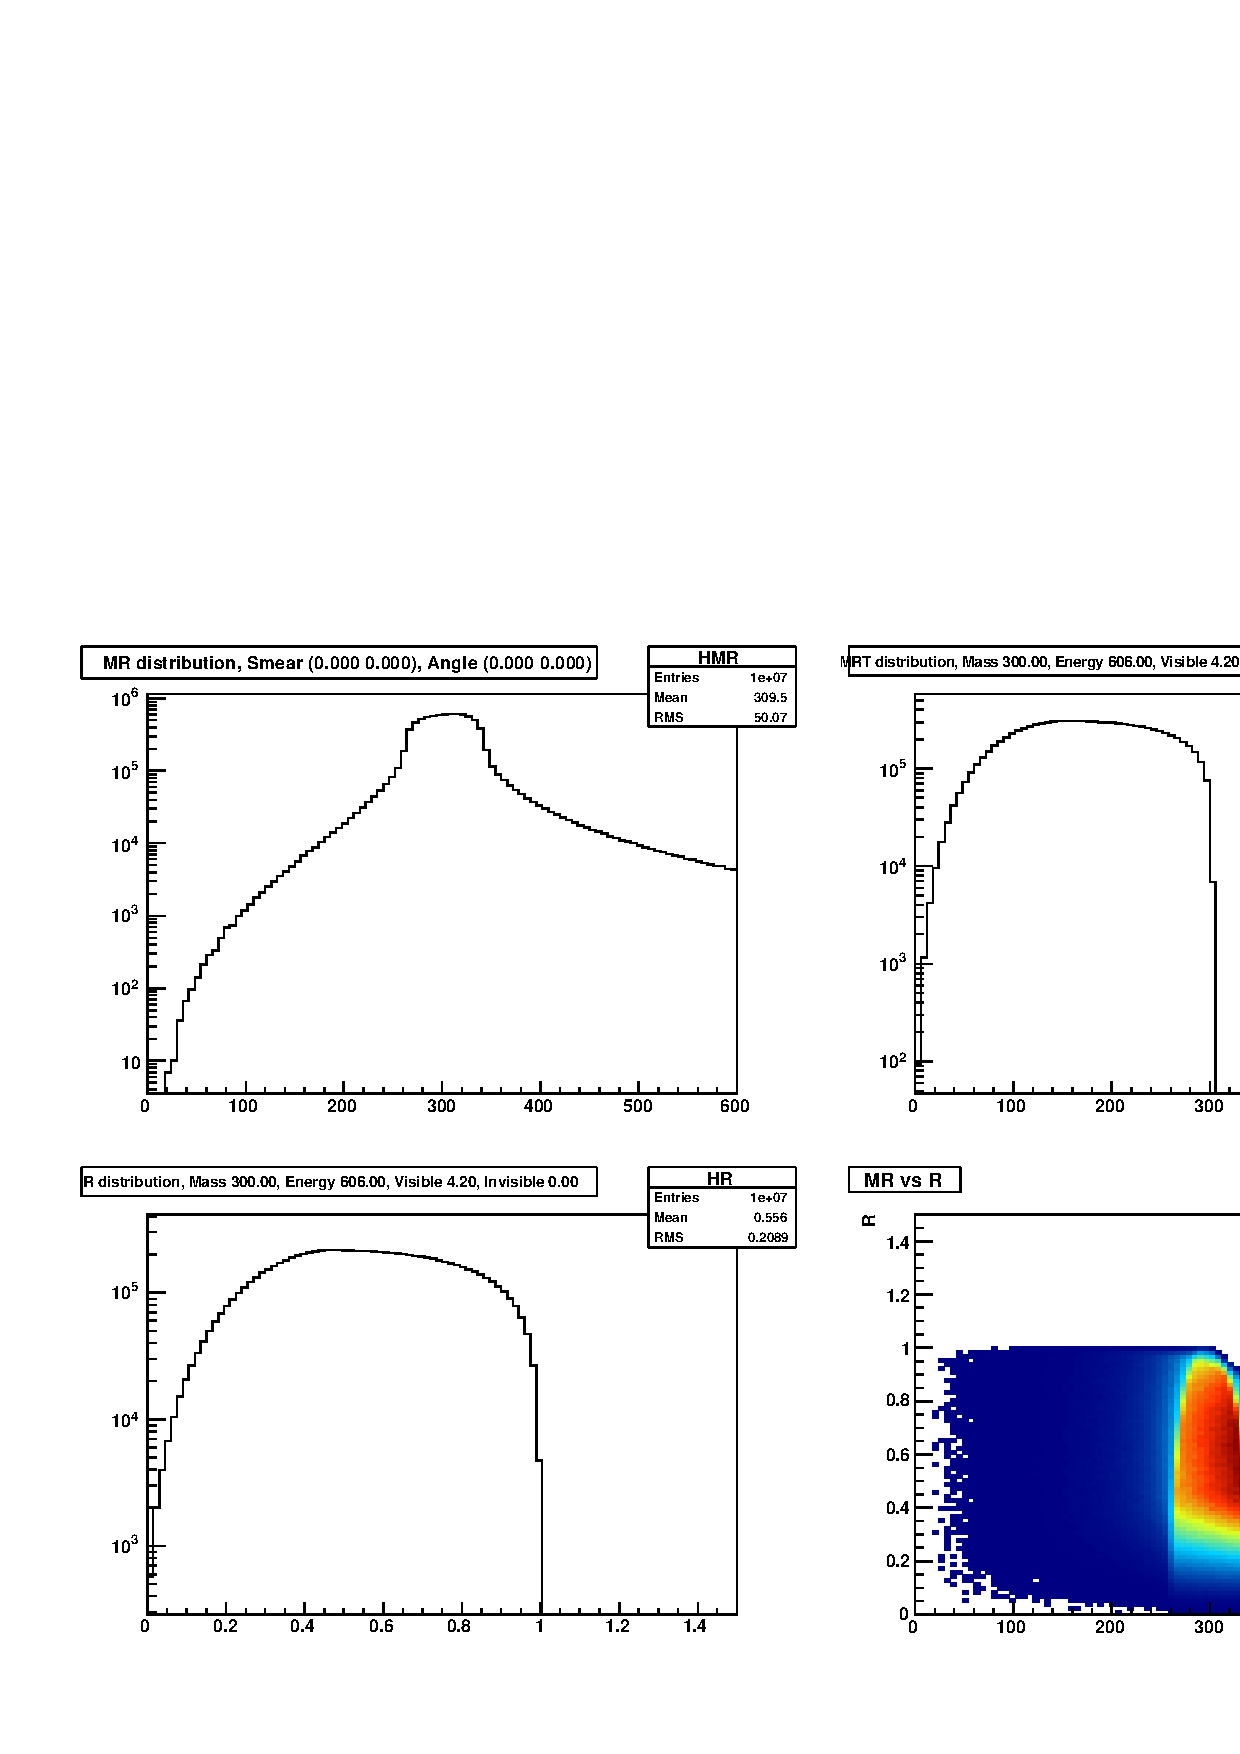
\includegraphics[width=7cm]{Figures/MRToy3_NoSmear}
   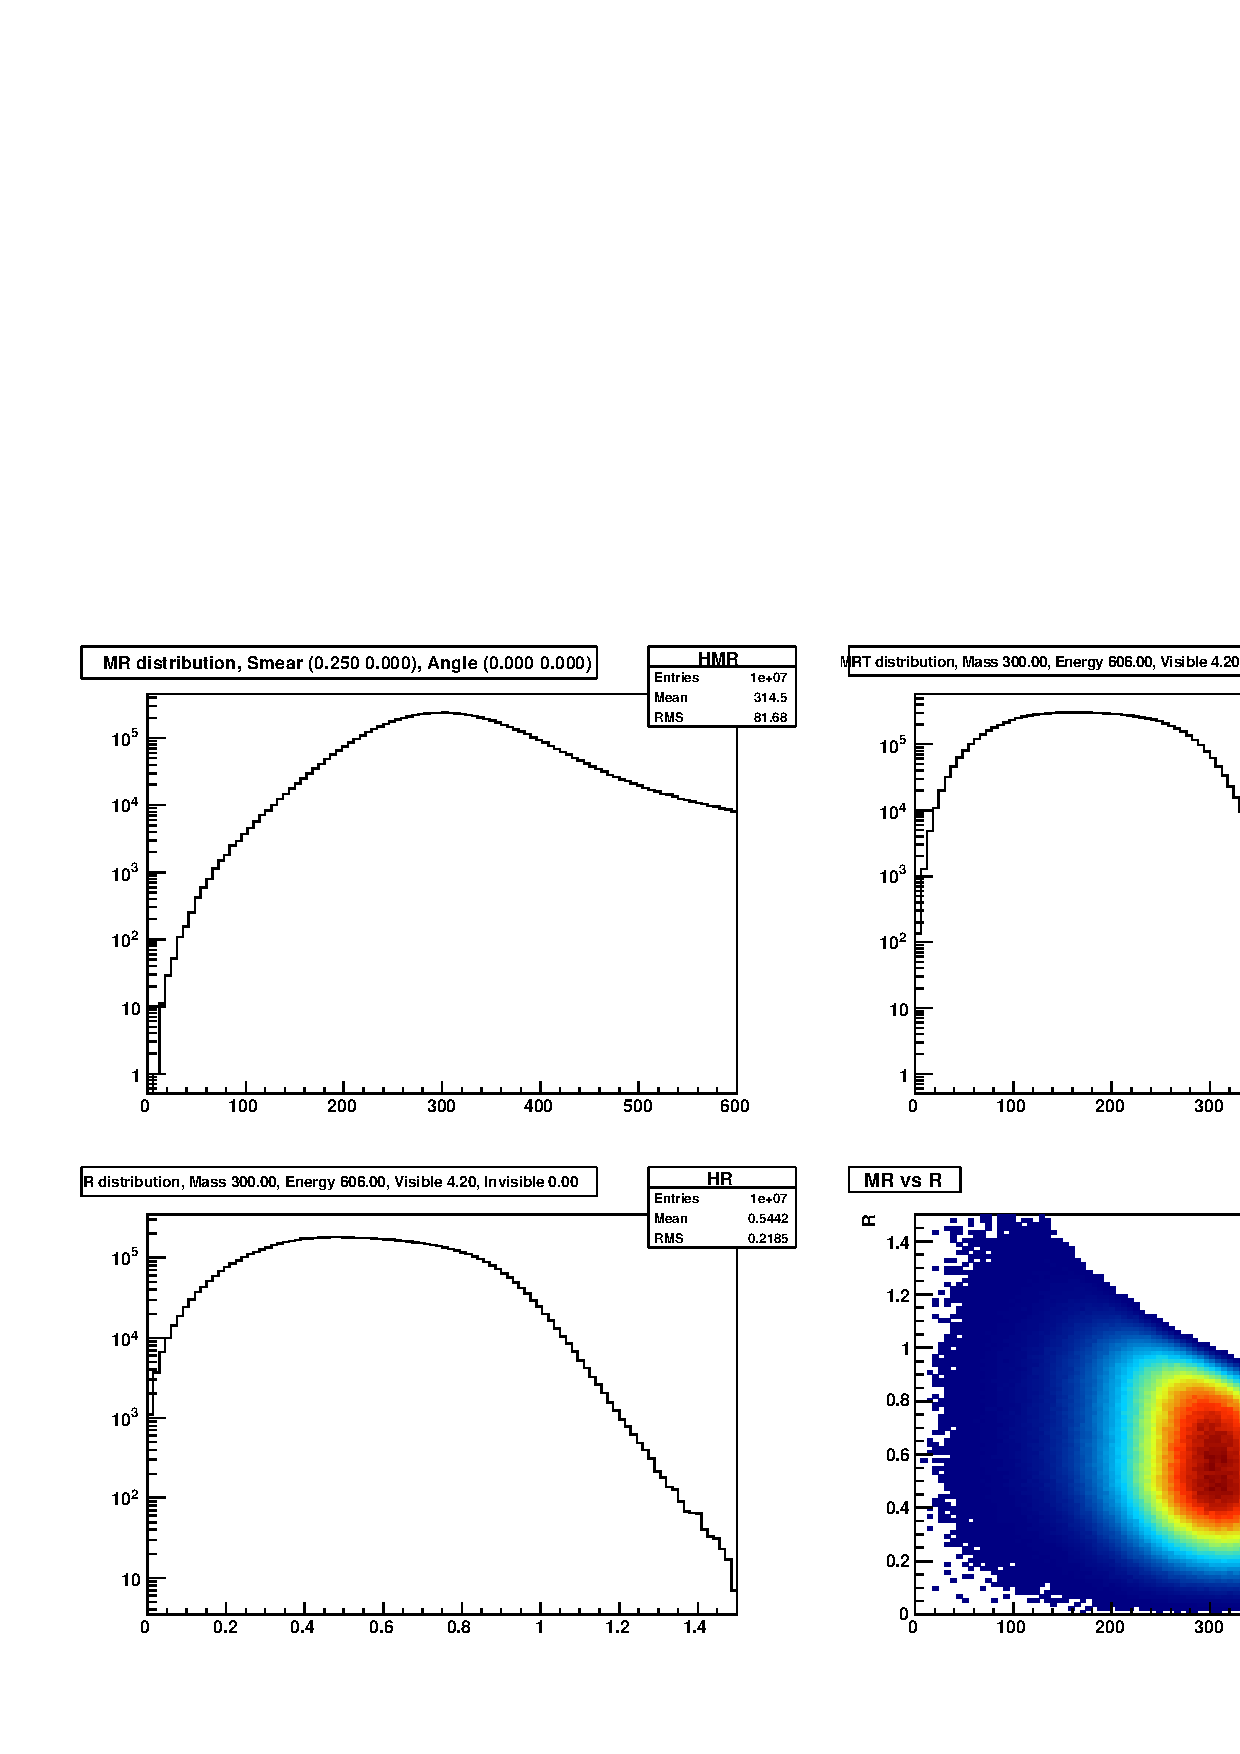
\includegraphics[width=7cm]{Figures/MRToy3_MomentumSmear}\\
   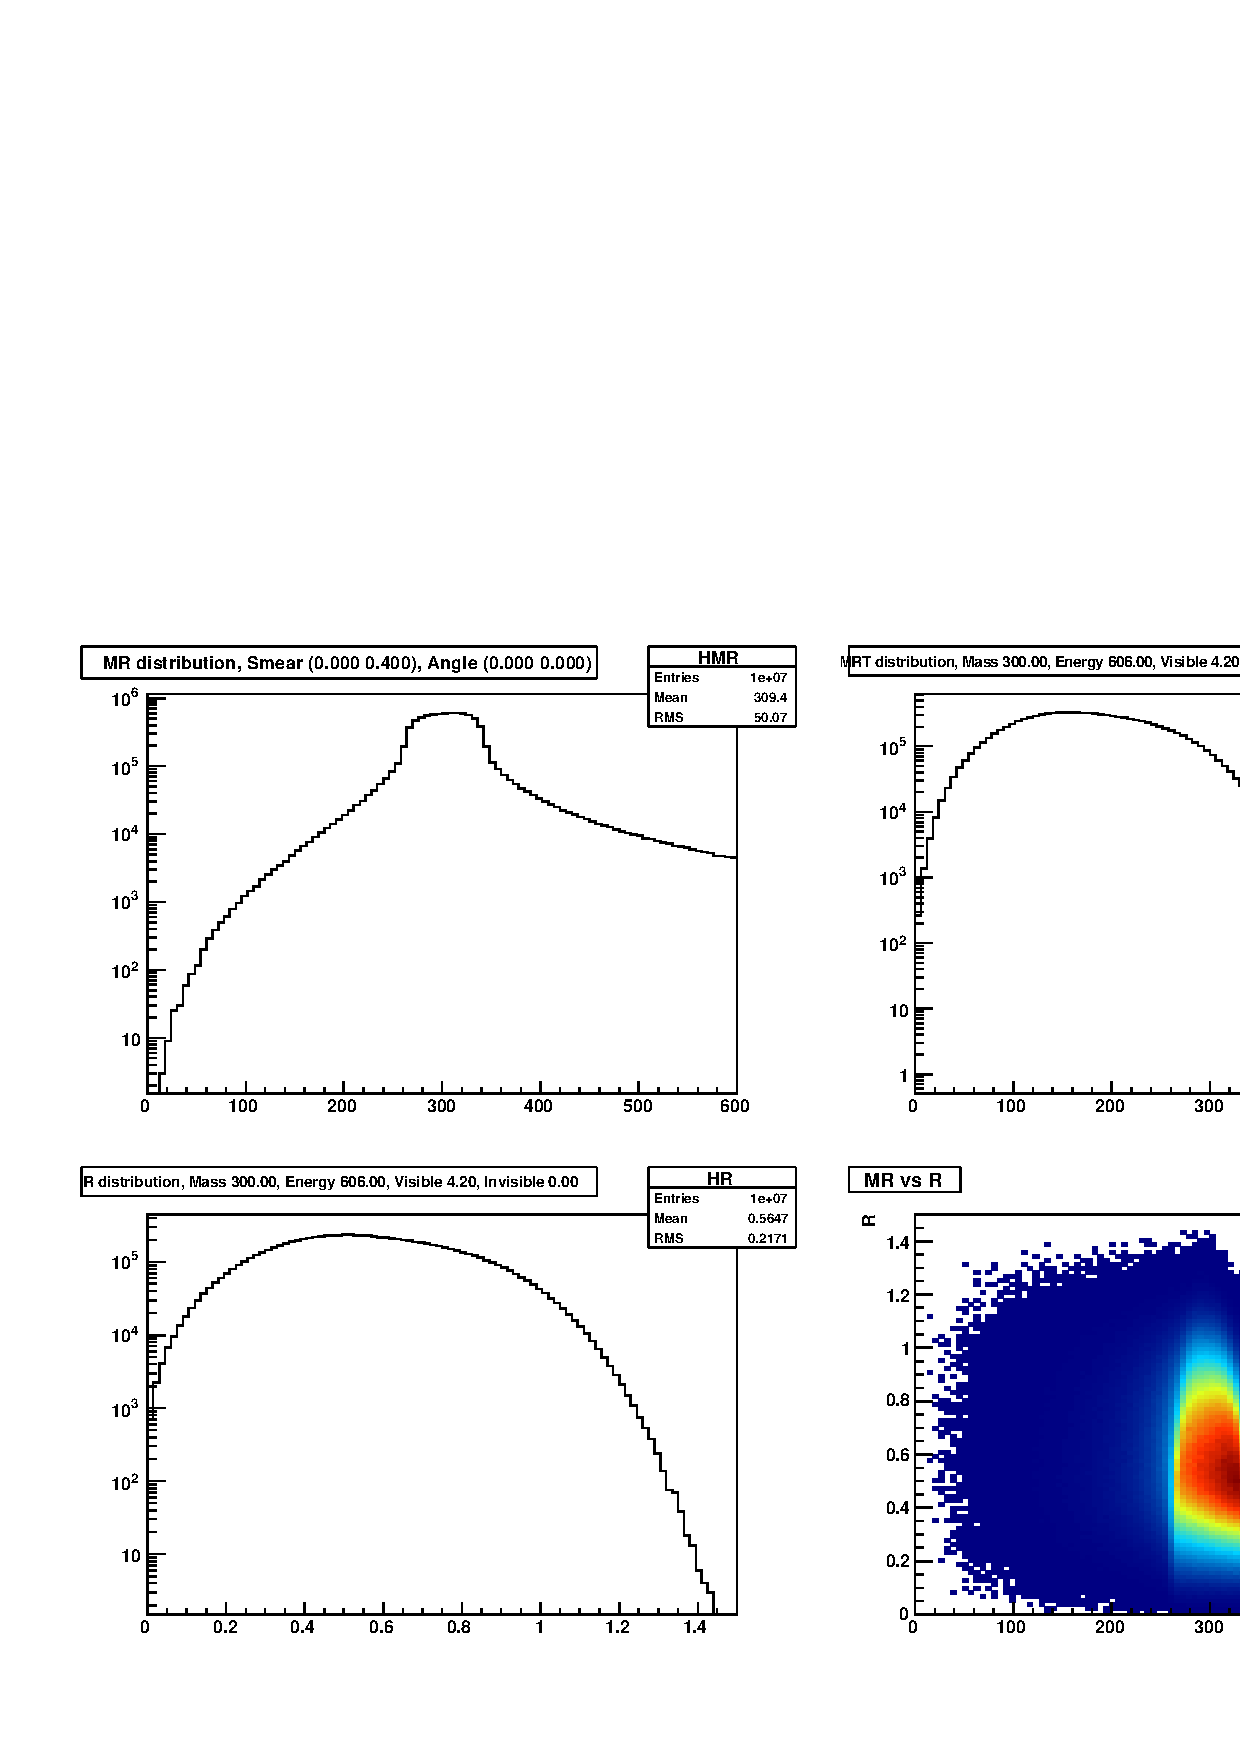
\includegraphics[width=7cm]{Figures/MRToy3_InvisibleMomentumSmear}
   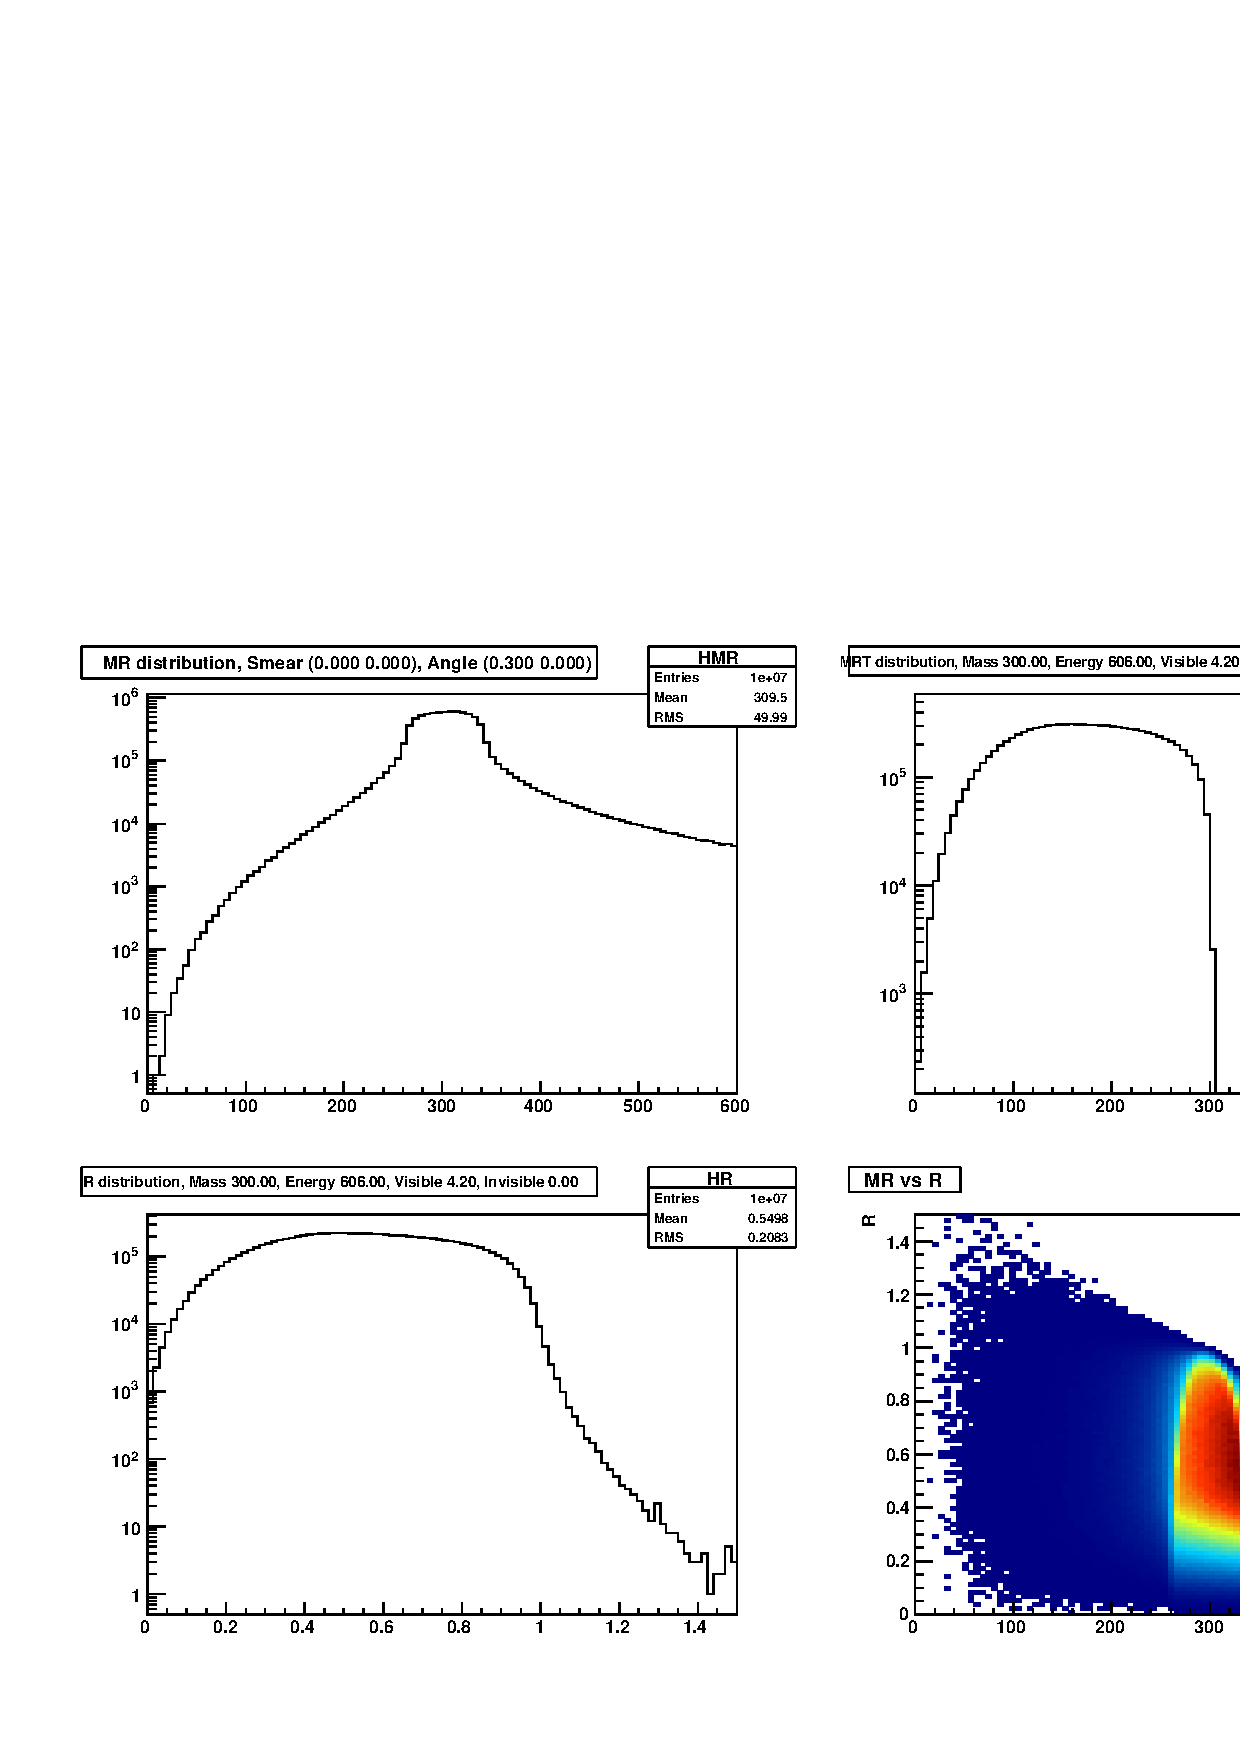
\includegraphics[width=7cm]{Figures/MRToy3_AngleSmear}
   \caption{Changing momentum scale/angle of final particles.  Upper left: no smear.  Upper right: scale of visible ones.  Lower Left: scale of invisible ones.  Lower right: angle of visible ones.}
   \label{Figure_MRToy3}
\end{figure}

\subsection{MRToy 5, transverse boost of whole system}

Some strange feature is forming when the hard-process is boosted in the transverse direction when the boost is moderately large, see figure \ref{Figure_MRToy5}.
The structure is not understood.  Let's leave it aside for now.
When boost is large, the two visible particle will tend to be closer and have larger momentum, so they will move to the lower-right corner.
Note that when the boost is huge it's not physical: there will be something balancing the hard process, and that something will be picked up by one of the hemispheres.

\begin{figure}[htbp]
   \centering
   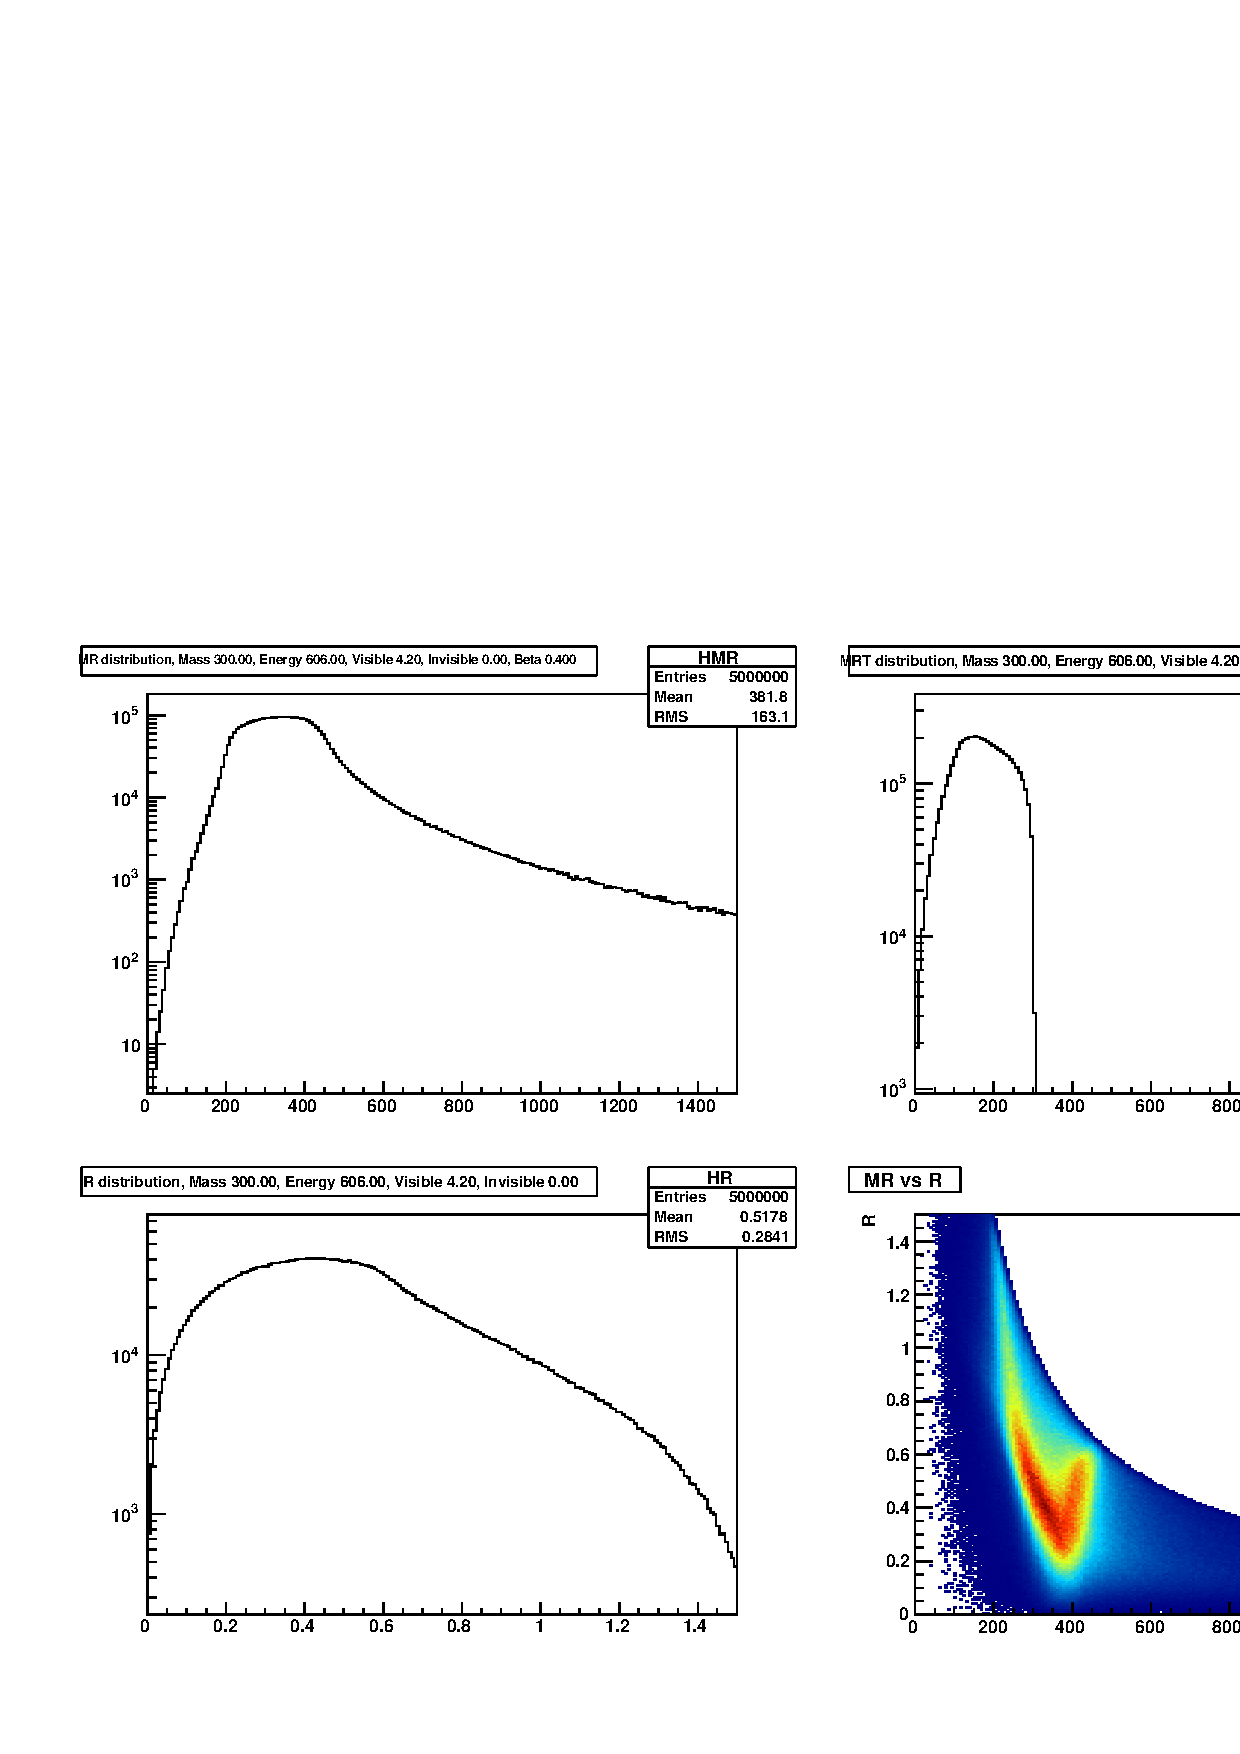
\includegraphics[width=7cm]{Figures/MRToy5_ModerateBoost}
   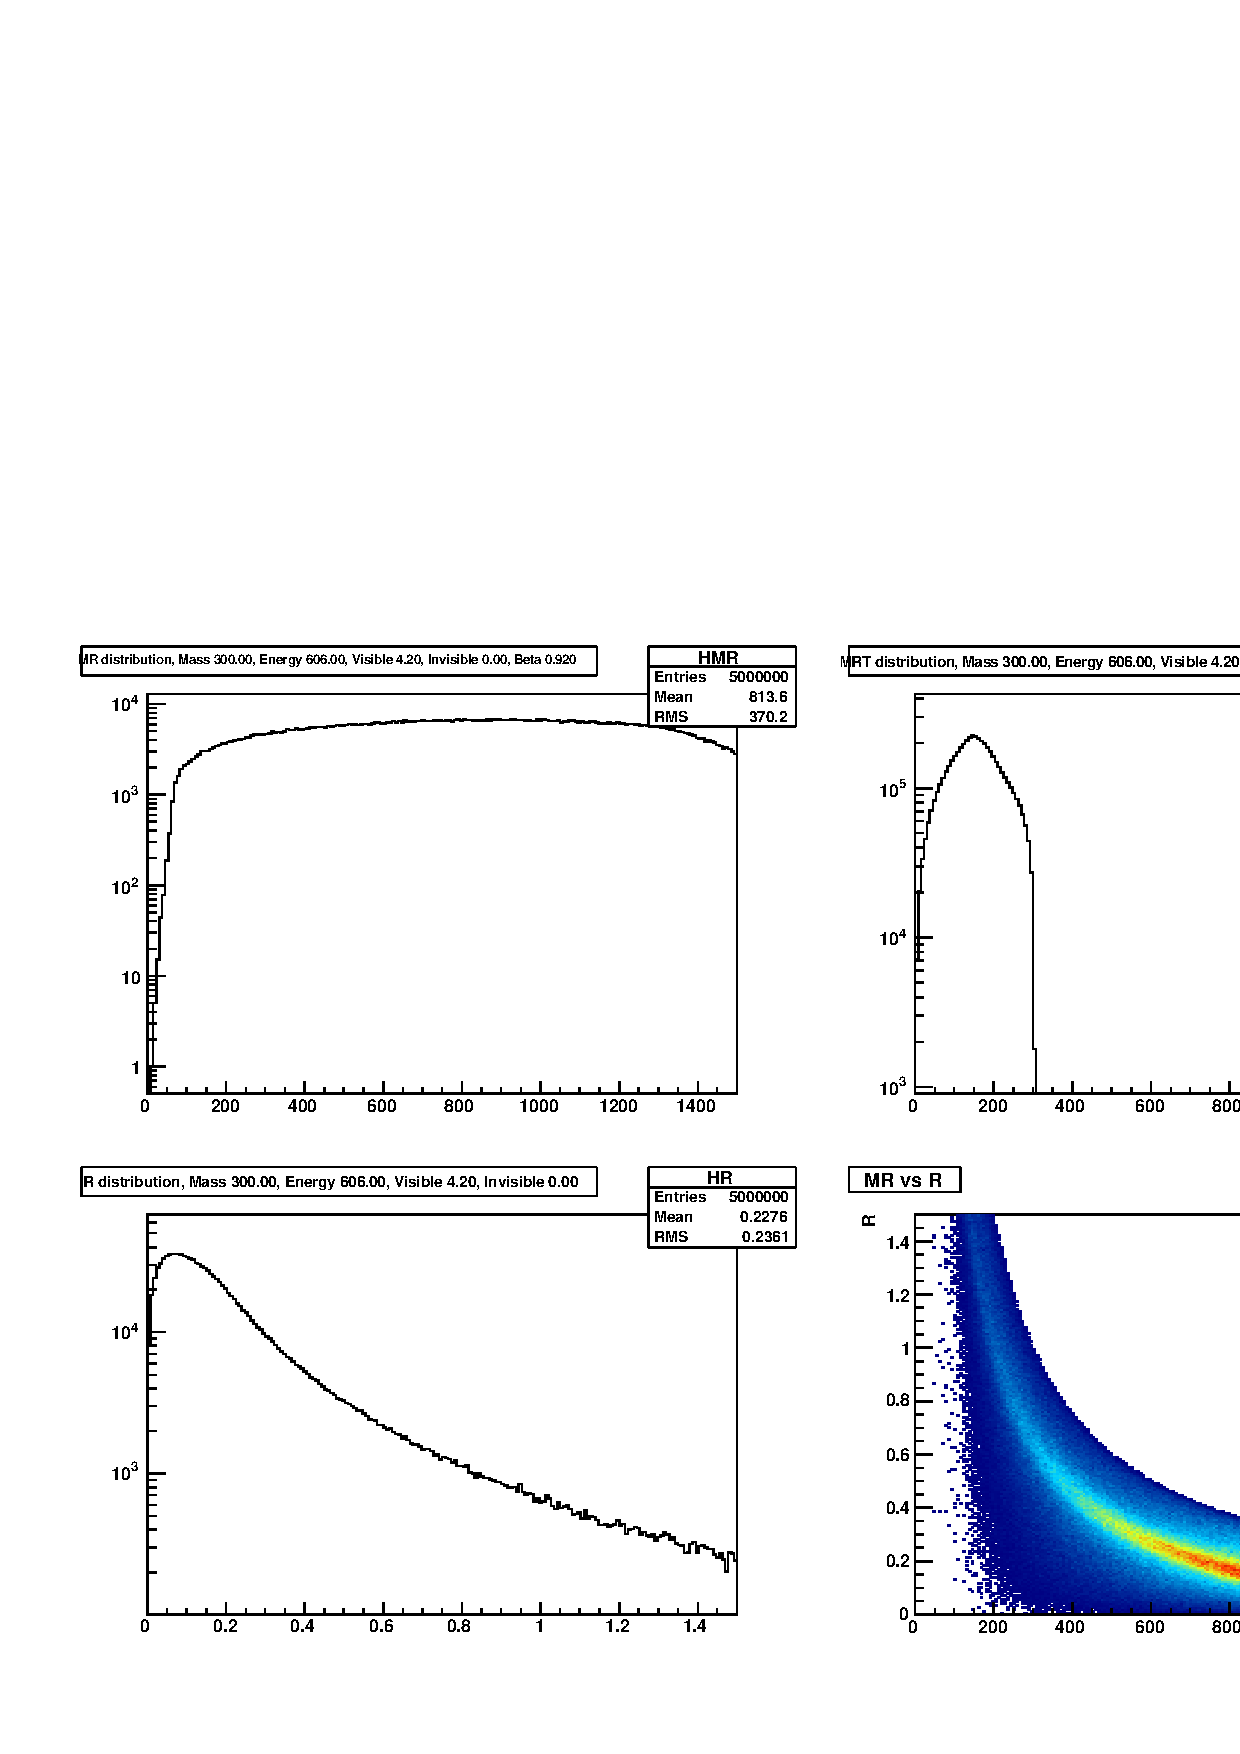
\includegraphics[width=7cm]{Figures/MRToy5_LargeBoost}
   \caption{Boost hard-process in the transverse direction.  Left: $\beta = 0.4$, Right: $\beta = 0.92$}
   \label{Figure_MRToy5}
\end{figure}

\subsection{MRToy 6, TTbar scenario, perfect assignment}

Changing mass of various objects.  It's all about sharing of energy among final particles, and that the invisible is assumed to be the same as visible.  See figure \ref{Figure_MRToy6}.
So when the neutrino mass is large, $M_R$ moves to the left since visible energy is smaller, and when lepton mass is large, $M_R$ becomes larger.

\begin{figure}[htbp]
   \centering
   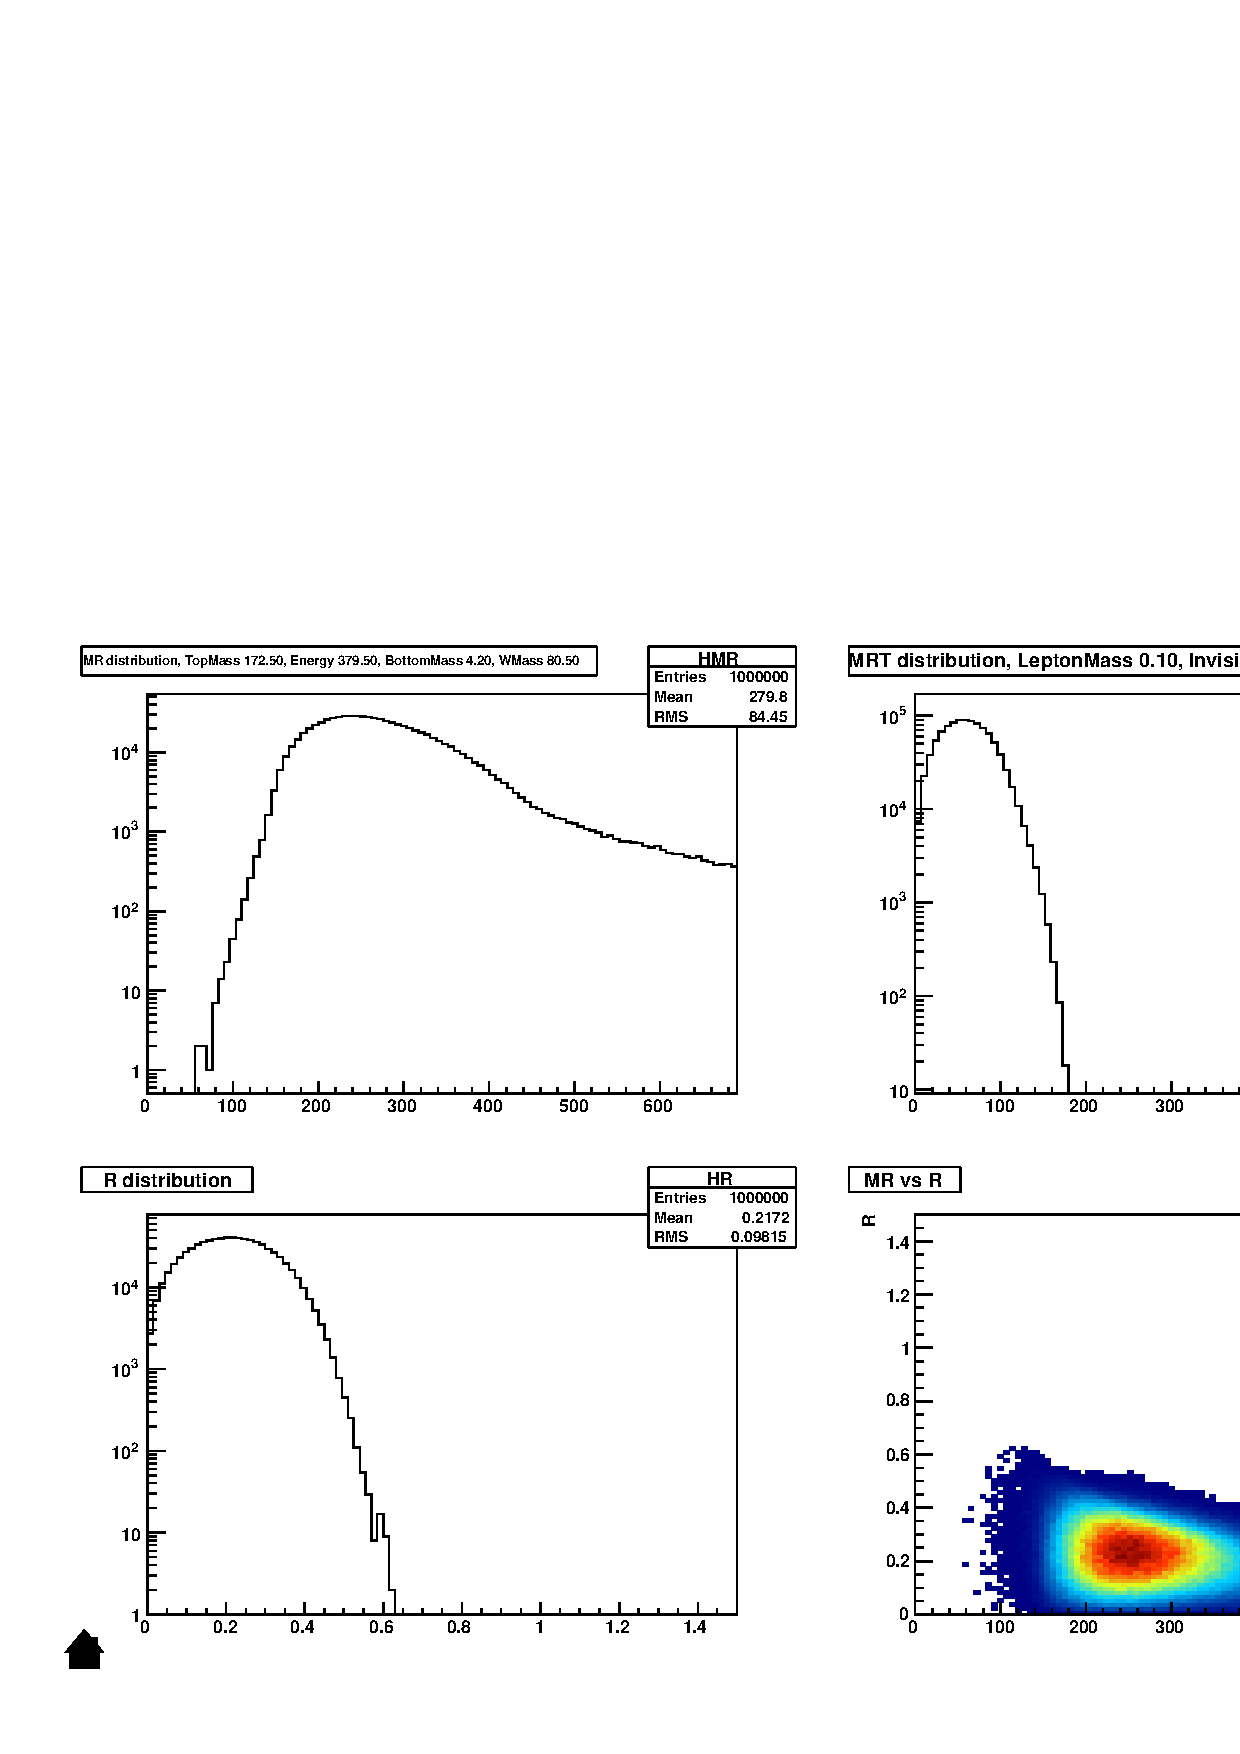
\includegraphics[width=7cm]{Figures/MRToy6_Realistic}
   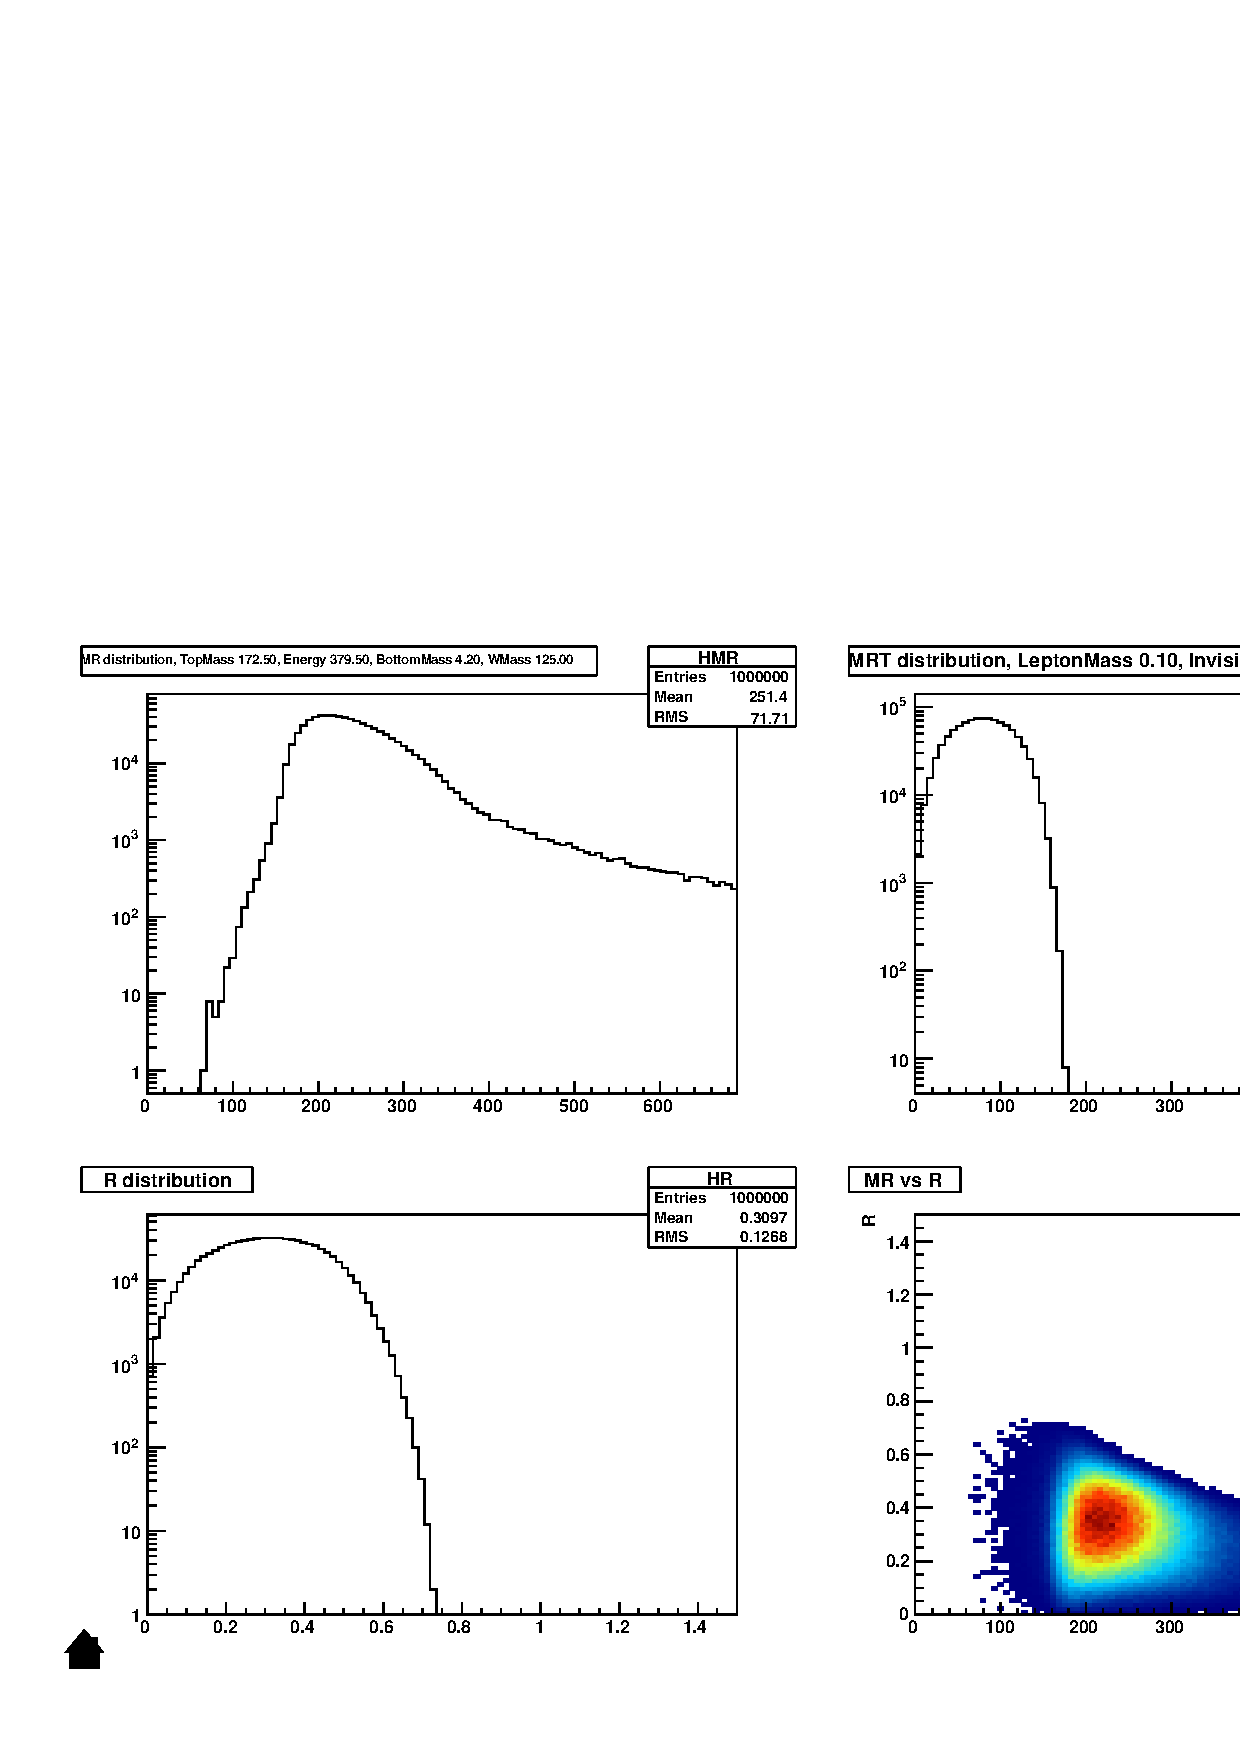
\includegraphics[width=7cm]{Figures/MRToy6_HeavyW}\\
   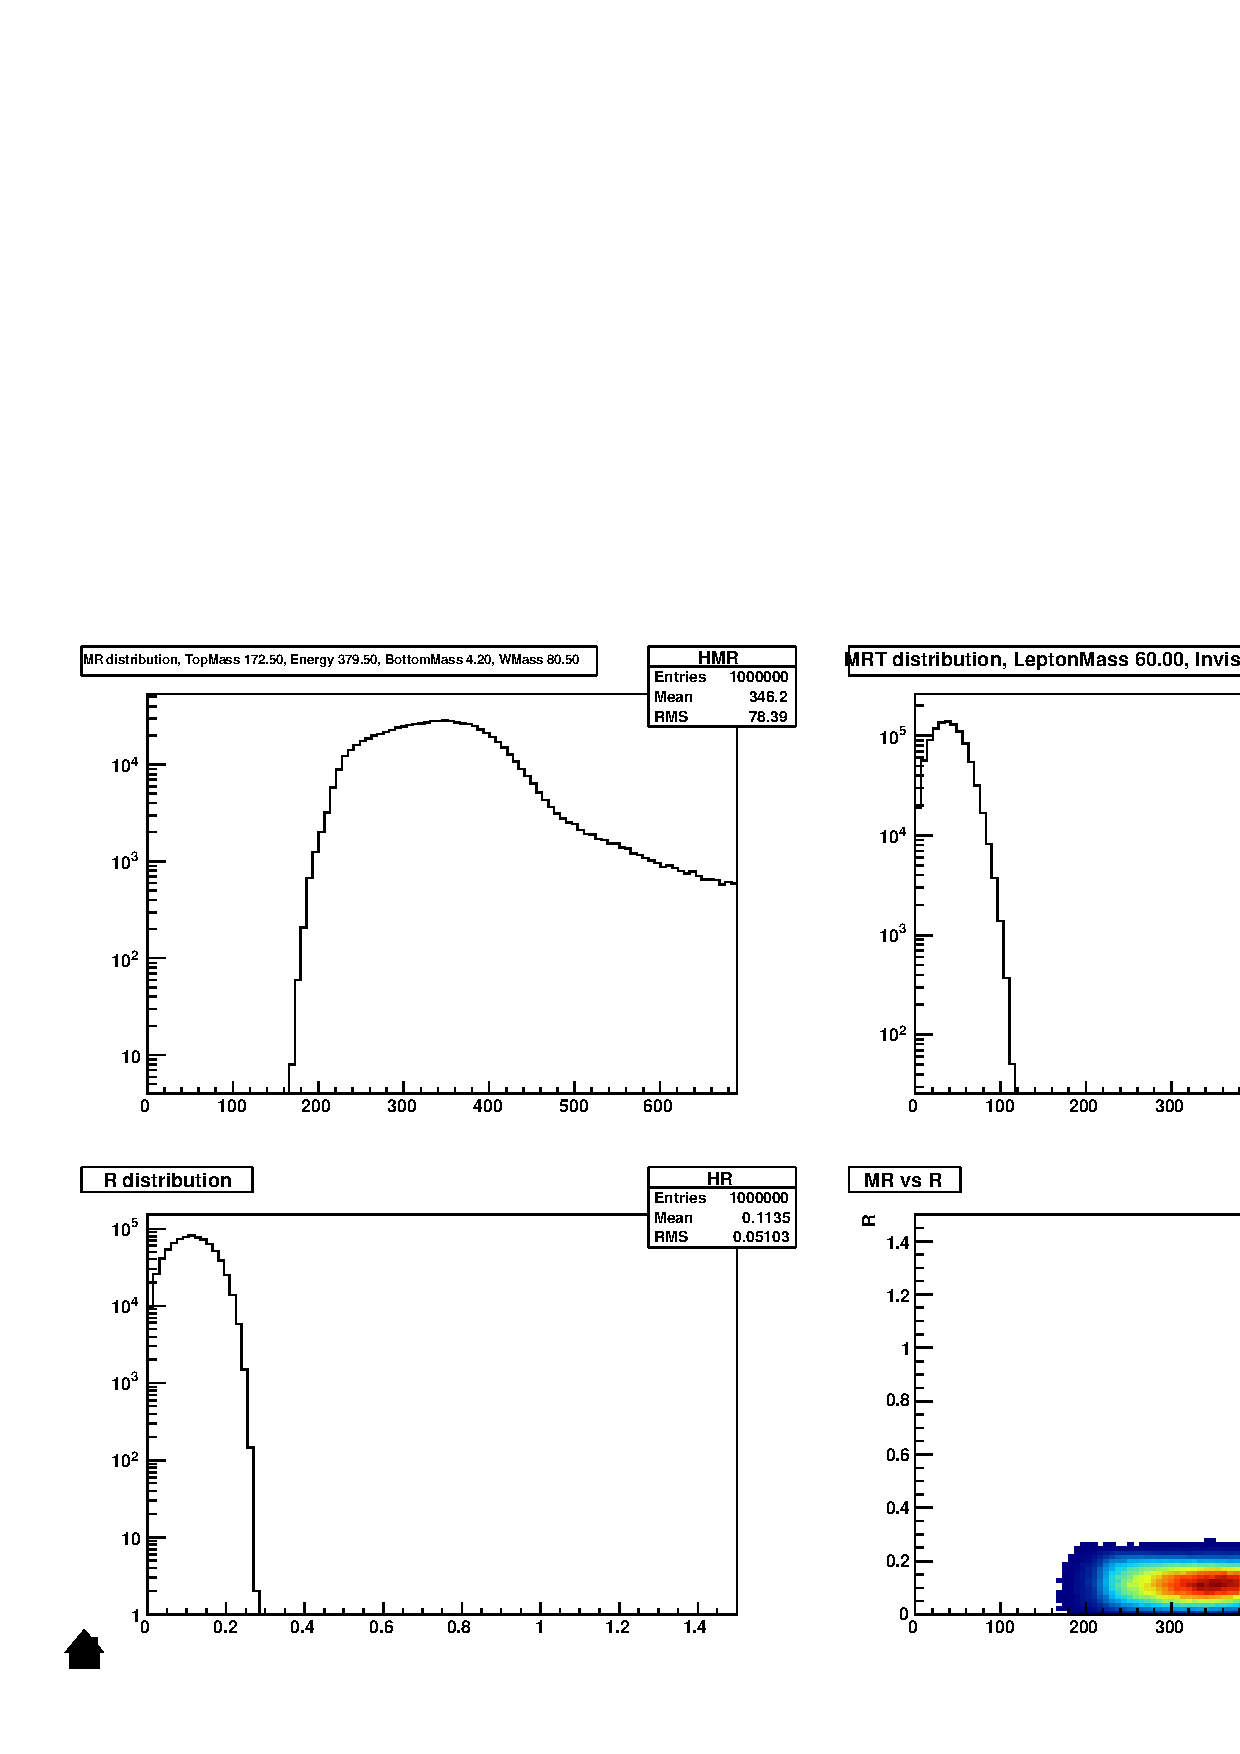
\includegraphics[width=7cm]{Figures/MRToy6_HeavyLepton}
   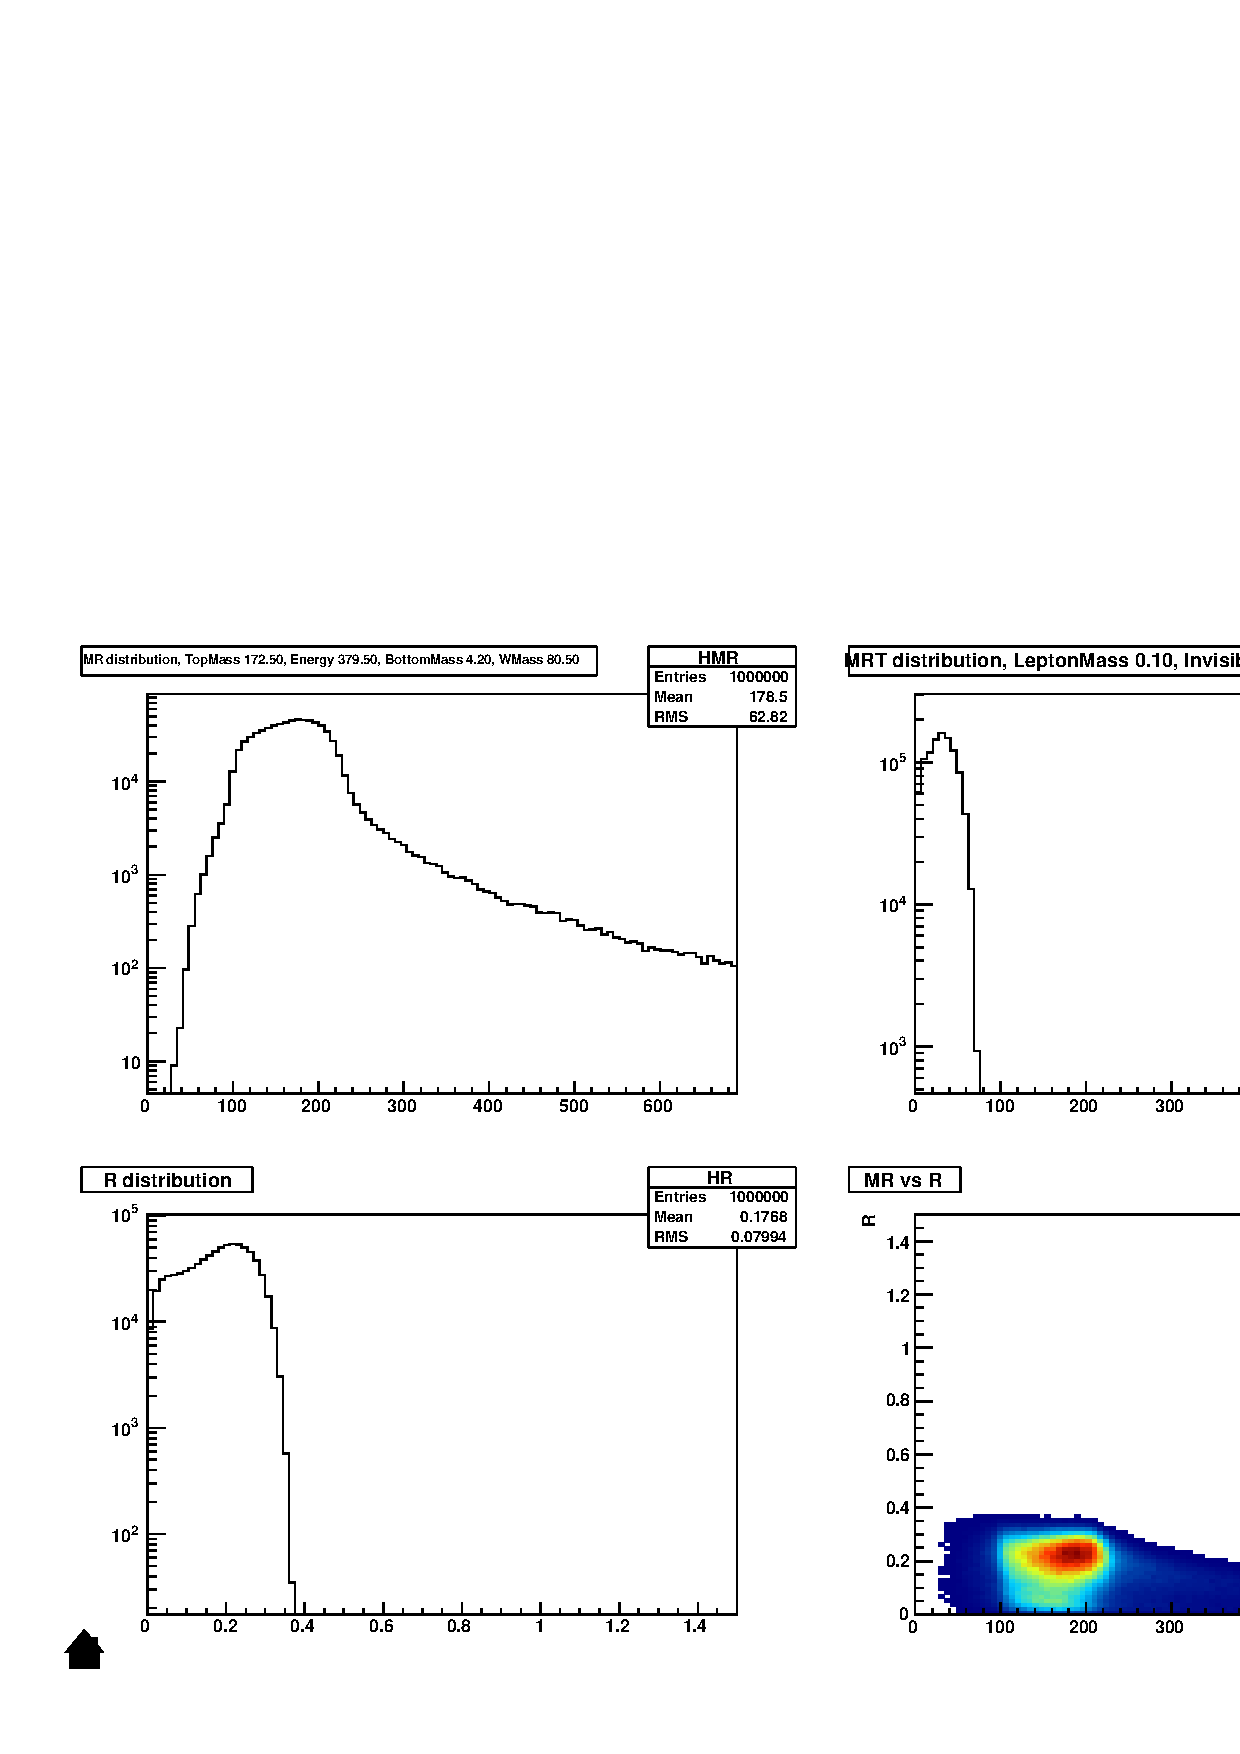
\includegraphics[width=7cm]{Figures/MRToy6_HeavyNeutrino}
   \caption{Changing masses in ttbar scenario.  Upper left: realistic situation.  Upper right: W is heavy.  Lower left: heavy lepton.  Lower right: heavy neutrino.}
   \label{Figure_MRToy6}
\end{figure}

\subsection{MRToy 8, adding a dijet from underlying event.  $M_R$ from leading jets}

Since we're picking out the first two jets and form Chris variables from them (at least the visible parts), we can see that there are
different combinations in the $M_R$ variable.  One peak at twice the jet momentum, one broad peak from hard process, and something inbetween for mixed.
when there is a large z-boost of the dijet, the mixed component gets larger than the other two combinations in $M_R$.
That's the tail extending to the lower-right corner in the $R-M_R$ plane.  See figure \ref{Figure_MRToy8}

\begin{figure}[htbp]
   \centering
   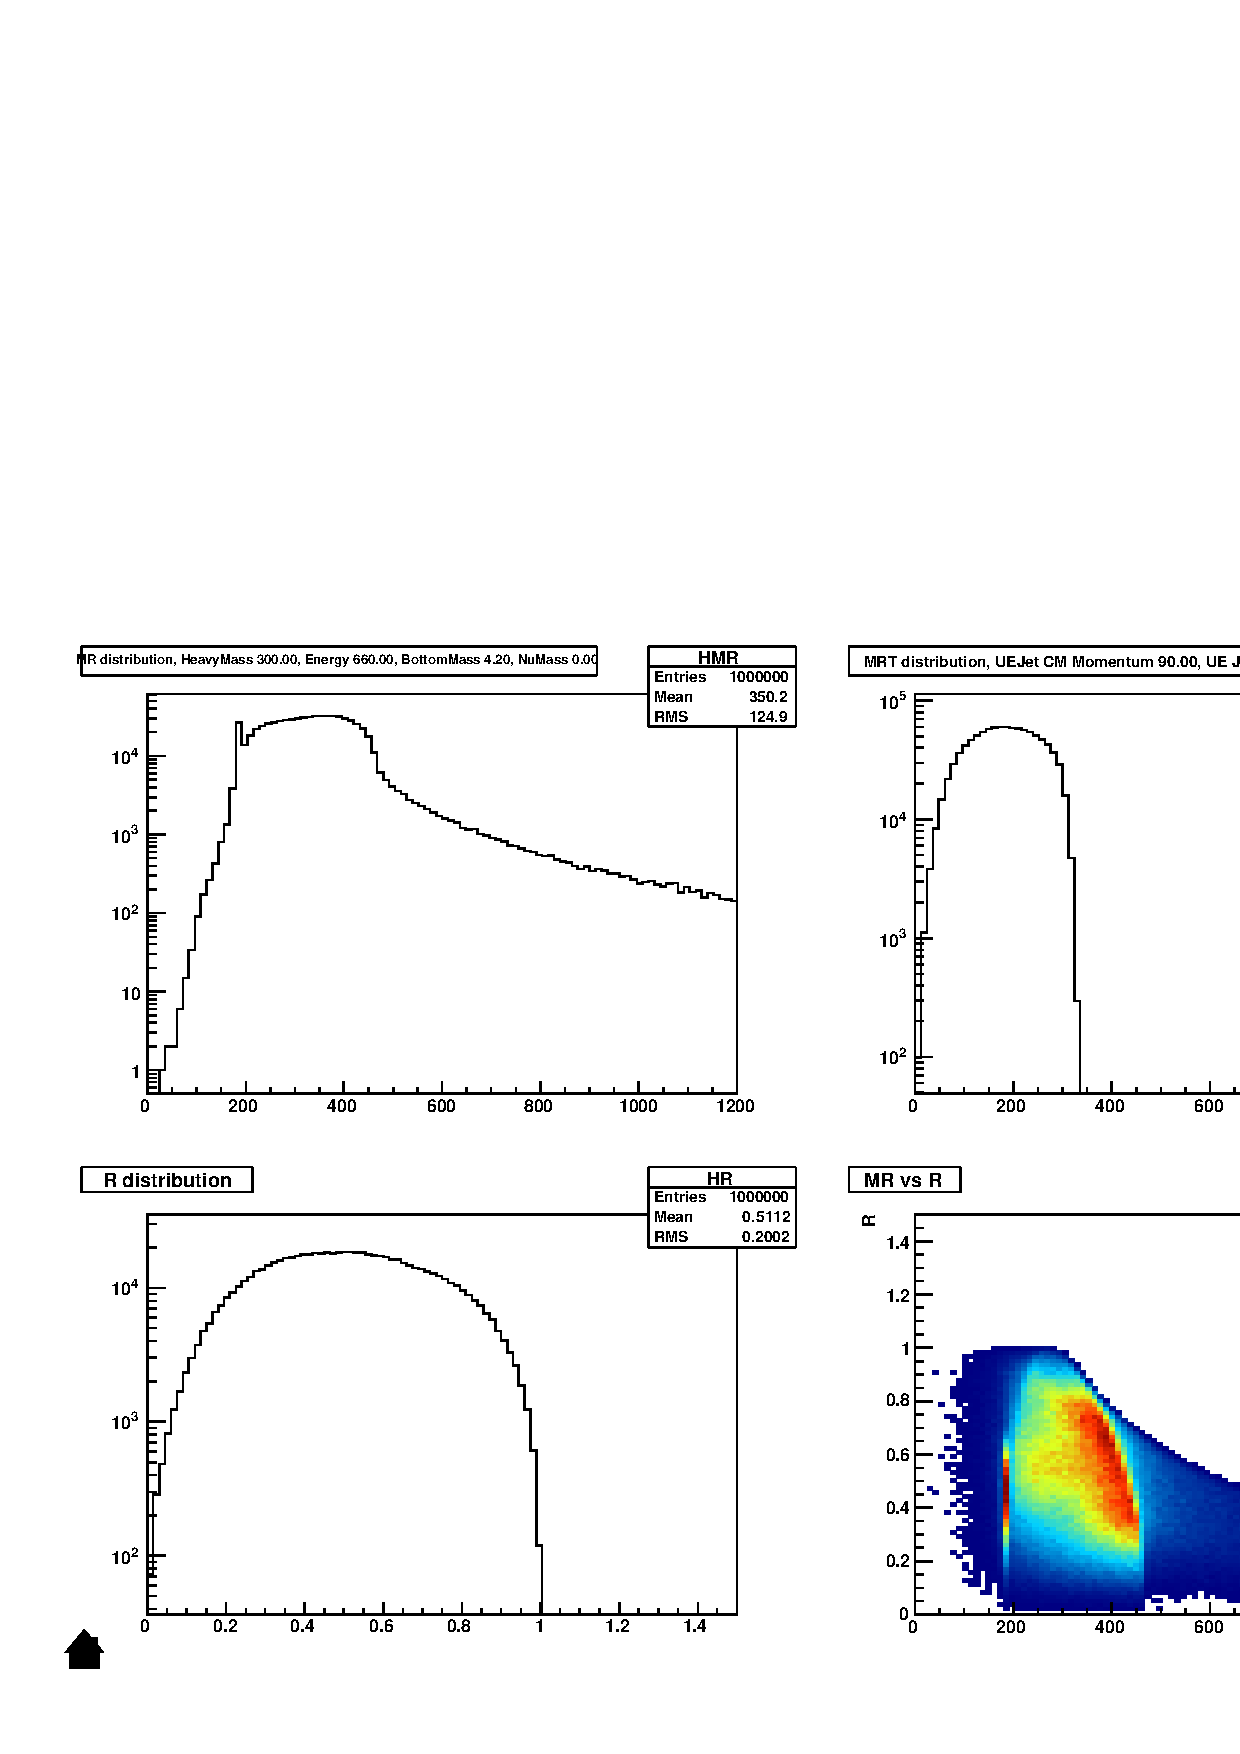
\includegraphics[width=7cm]{Figures/MRToy8_SmallJet}
   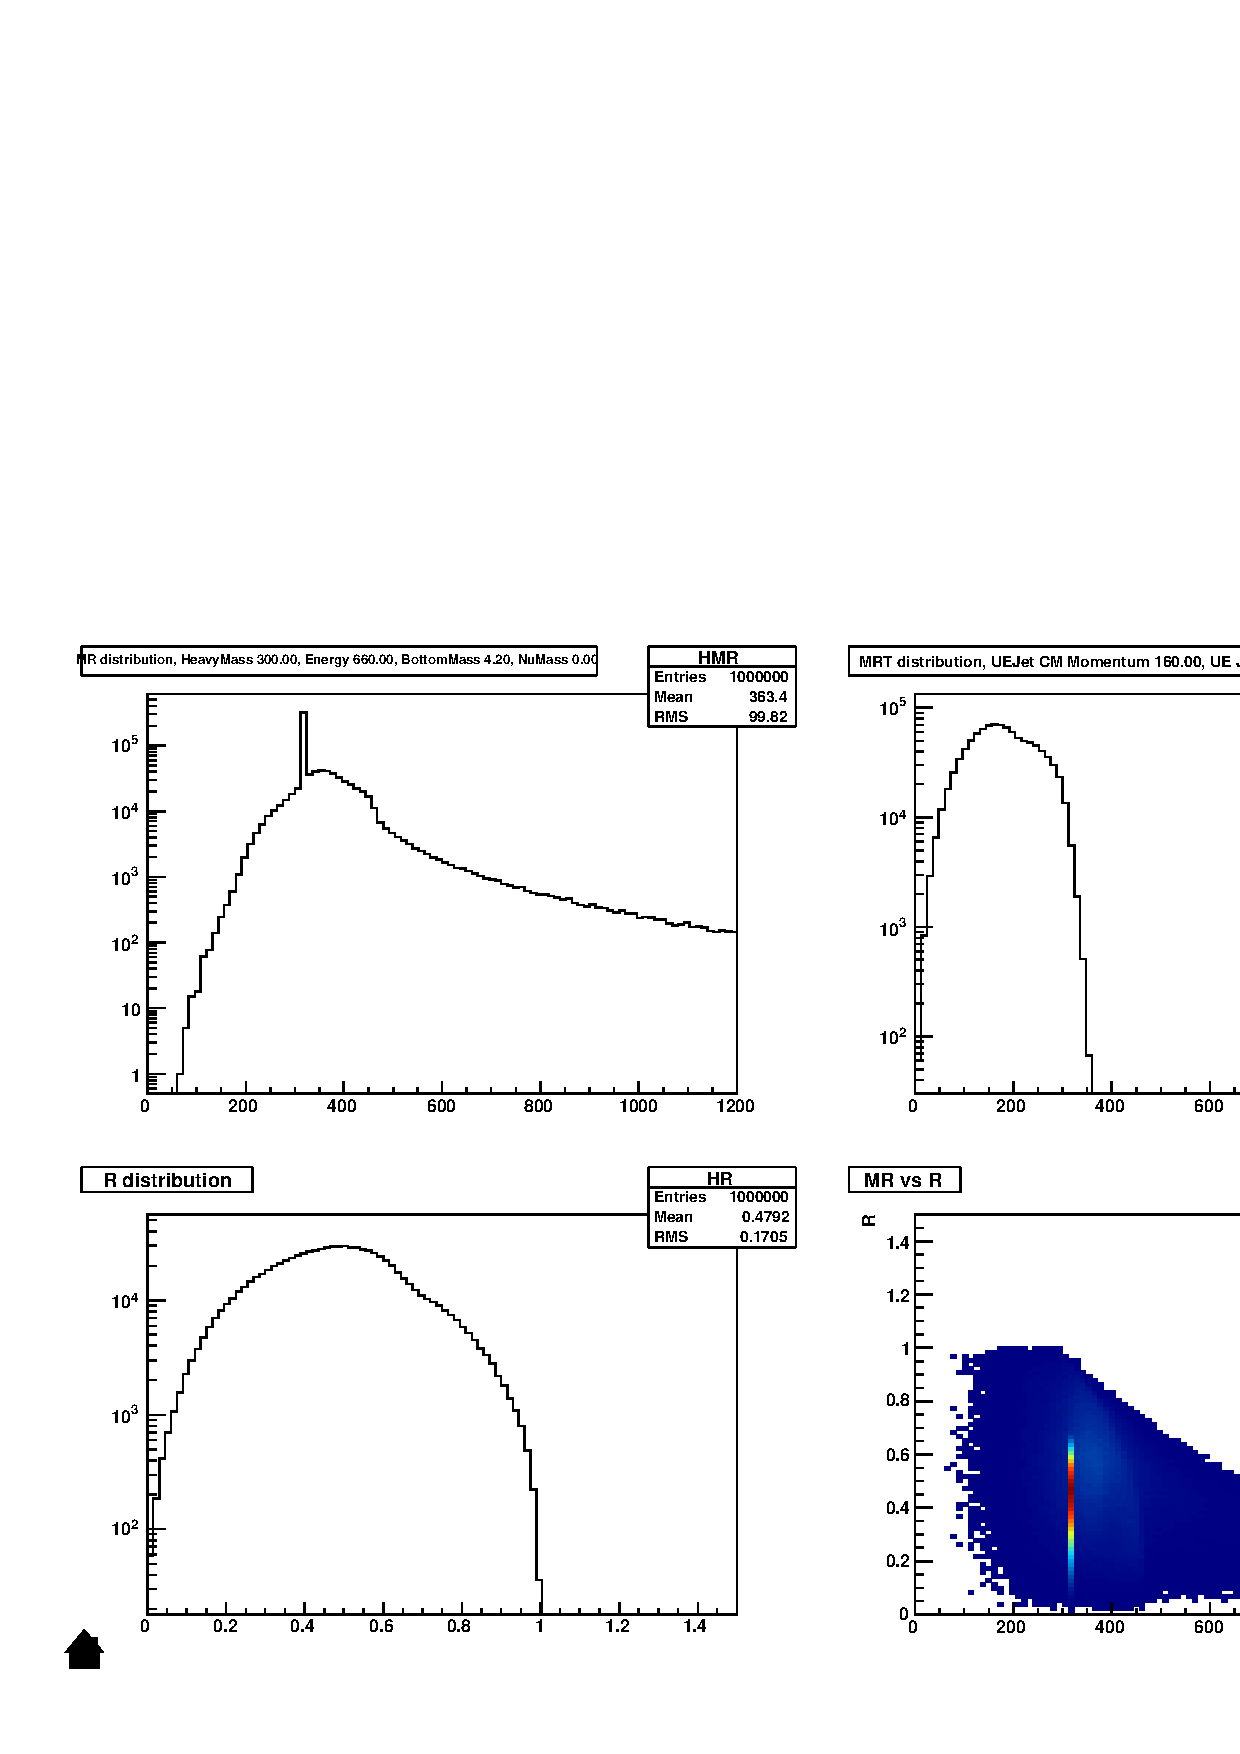
\includegraphics[width=7cm]{Figures/MRToy8_LargeJet}\\
   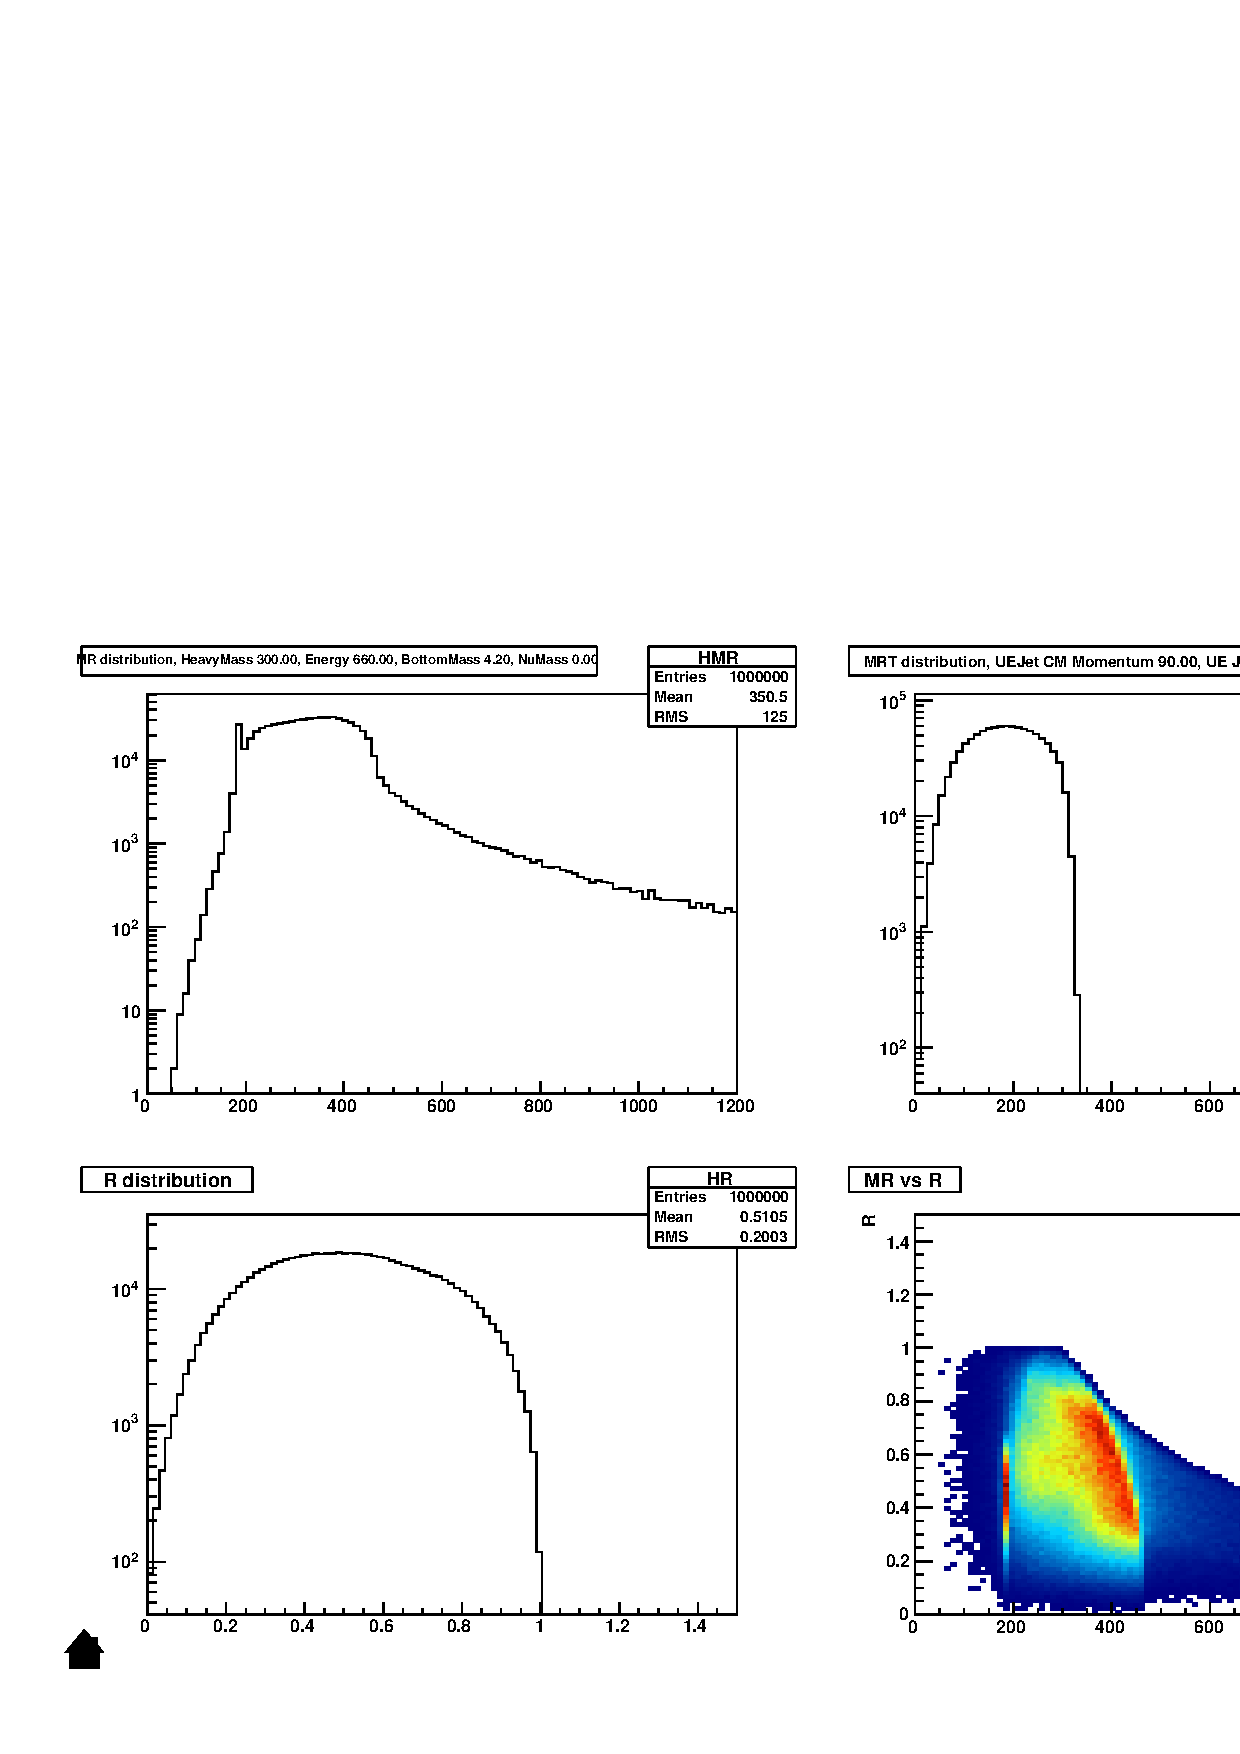
\includegraphics[width=7cm]{Figures/MRToy8_SmallBoost}
   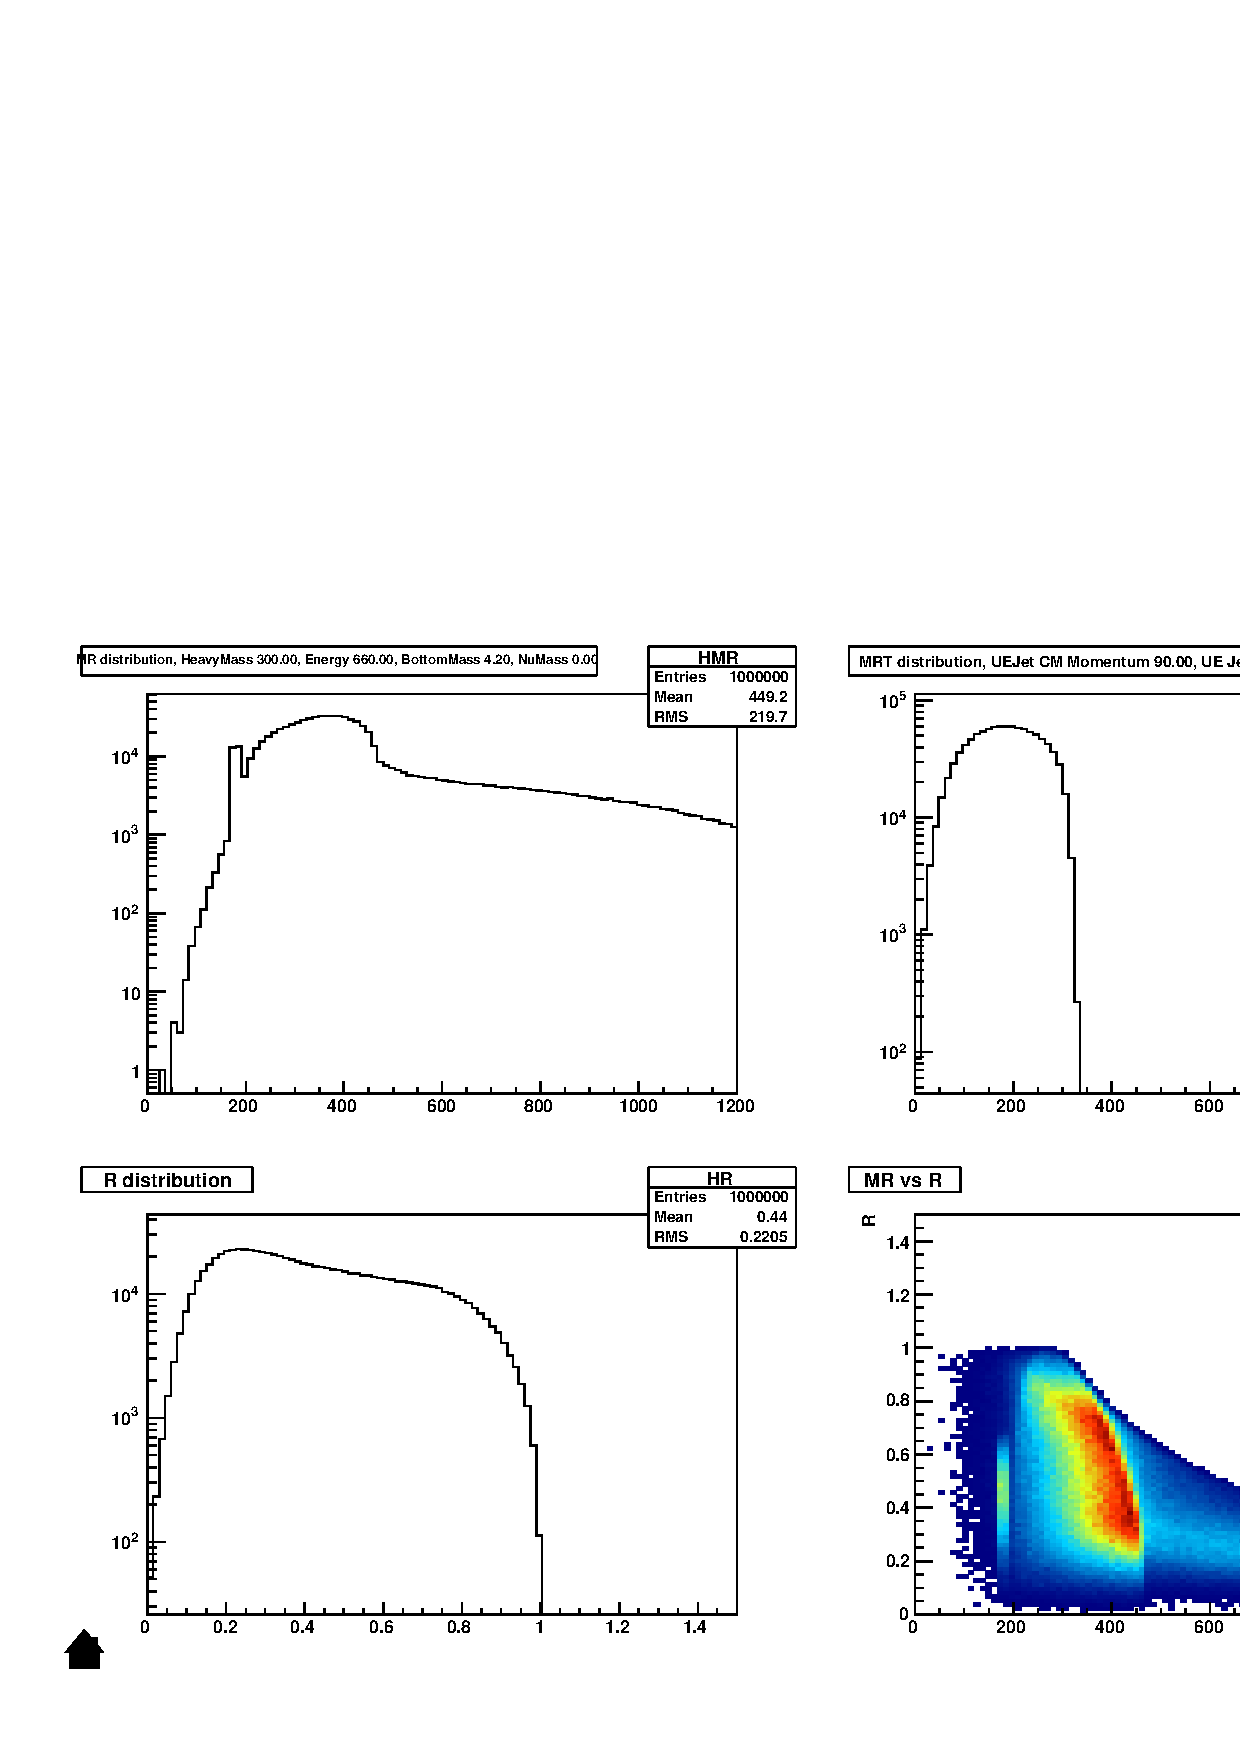
\includegraphics[width=7cm]{Figures/MRToy8_LargeBoost}
   \caption{Adding dijet from UE.  Upper left: small extra jet (90).  Upper right: large extra jet (160).  Lower left: Small z-boost of the dijet.  Lower right: large z-boost}
   \label{Figure_MRToy8}
\end{figure}

\subsection{MRToy 9, adding a dijet from underlying event.  $M_R$ from hemispheres}

Similar as before, except that the energy are added to form hemispheres.  Due to the assumption of invisible particles in the $M_R$ variable, $M_R$ increases accordingly.
Not too interesting too look at.  In figure \ref{Figure_MRToy9} we can see the it moves.

\begin{figure}[htbp]
   \centering
   \includegraphics[width=7cm]{Figures/MRToy9_SmallJet}
   \includegraphics[width=7cm]{Figures/MRToy9_LargeJet}
   \caption{Adding dijet from UE.  Left: small extra jet.  Right: large extra jets.}
   \label{Figure_MRToy9}
\end{figure}

\subsection{MRToy 10.  Adding ISR jet balancing the whole system}

Variables constructed by the leading two jets, so we can see more action (figure \ref{Figure_MRToy10}).  Not much added information, though it's fun to look.

\begin{figure}[htbp]
   \centering
   \includegraphics[width=7cm]{Figures/MRToy10_SmallISRJet}
   \includegraphics[width=7cm]{Figures/MRToy10_LargeISRJet}
   \caption{Adding ISR jet.  Left: small extra jet.  Right: large extra jets.}
   \label{Figure_MRToy10}
\end{figure}


\subsection{MRToy 13.  Adding transverse ISR jet balancing the whole system}

Since longitudinal boost doesn't matter, let's look at the transverse ISR-balancing jet for now.  Group things into hemispheres also, while I'm at it.
First of all there are two ways to group three things (since each hemisphere is required to have something at least), and that's why we see two-peaked structure in the result.
In the case of small ISR jet, it's unusual to have one group containing two jets from hard process, and therefore it is fainter.
When the boost (ISR jet size) is large, the energy scale will increase and push $M_R$ to higher values.

\begin{figure}[htbp]
   \centering
   \includegraphics[width=7cm]{Figures/MRToy13_SmallISRJet}
   \includegraphics[width=7cm]{Figures/MRToy13_LargeISRJet}
   \caption{Adding transverse ISR jet.  Left: small extra jet.  Right: large extra jets.}
   \label{Figure_MRToy13}
\end{figure}




\section{Summary}

A list of toys on Chris' kinematic variable has been documented here with summary plots for each of them.
It's useful in building intuition about these variables.  I hope.



% \begin{thebibliography}{9}
%    \bibitem{Yay} {\bf Yay Yay Yay},
%       Y. Yayayaya,
%       {\em "Yayayayay study using 2010 data"}
% \end{thebibliography}
 
\pagebreak

\end{document}

